%% Page de garde %%
\documentclass[a4paper, 12pt]{article}

\title{Rapport de projet}
\author{Hugo Meleiro}

\usepackage[french]{babel}
\usepackage{csquotes}
\usepackage{lipsum}
\usepackage{setspace}
\usepackage[hidelinks]{hyperref}
\usepackage[nottoc]{tocbibind}
\setlength{\emergencystretch}{2em}

\usepackage{caption}
\usepackage{subcaption}
\usepackage{ulem}
\normalem

\usepackage[margin=25mm]{geometry} 
\usepackage{graphicx}
\usepackage{pdfpages} 
\usepackage{afterpage}
\newcommand\myemptypage{
    \null
    \thispagestyle{empty}
    \addtocounter{page}{-1}
    \newpage
}

\setlength{\parindent}{0em}
\setlength{\parskip}{1em}


\usepackage{pgfplots} 
\pgfplotsset{width=7cm, compat=newest}
\usetikzlibrary{patterns}
\usepackage{bchart}
\renewcommand{\bcfontstyle}{}
\usepackage{pgf-pie}
\usepackage{float}
\usepackage{xcolor}
\usepackage{pdfpages}
\definecolor{codegreen}{rgb}{0,0.6,0}
\definecolor{codegray}{rgb}{0.5,0.5,0.5}
\definecolor{codepurple}{rgb}{0.68,0,0.12}
\definecolor{backcolour}{rgb}{0.96,0.96,0.96}

\usepackage{listings}
\lstloadlanguages{csh}
\lstdefinestyle{mystyle}{
    backgroundcolor=\color{backcolour},
    commentstyle=\color{codegray},
    keywordstyle=\color{codepurple},
    numberstyle=\tiny\color{codegray},
    stringstyle=\color{codegreen},
    basicstyle=\ttfamily\footnotesize,
    breakatwhitespace=false,
    breaklines=true,
    captionpos=b,
    keepspaces=true,
    numbers=left,
    numbersep=5pt,
    showspaces=false,
    showstringspaces=false,
    showtabs=false,
    tabsize=2,
    literate={á}{{\'a}}1 {ã}{{\~a}}1 {é}{{\'e}}1 
}

\lstset{style=mystyle}

%% DEBUT %%
\usepackage[T1]{fontenc}
\begin{document}

\pagenumbering{roman}

\begin{titlepage}
    \vbox{ }

    \vbox{ }

    \begin{center}
        % Over-titre
        
\includegraphics[width=0.40\textwidth]{img/logos/logo.png}\\[1cm]
        \textsc{\Large Rapport de Projet}\\[0.2cm]
        \textsc{\Large Robot suiveur de ligne - 2022/2023}\\[0.6cm]

        % \vbox{ }
        % Titre
        \noindent\makebox[\linewidth]{\rule{.7\paperwidth}{.6pt}}\\[0.7cm]
        { \huge \bfseries goofyBot - Coochie Team}\\[0.25cm]
        \noindent\makebox[\linewidth]{\rule{.7\paperwidth}{.6pt}}\\[0.7cm]
        \large{\bfseries Créé par :}\\[0.1cm]
        \large{Hugo Meleiro}\\[0.1cm]
        \large{Marius Deias}\\[0.1cm]
        \large{Matthieu Haddad}\\[0.1cm]
        \large{Bilel Tangour}\\[0.5cm]
        \large{Responsables : M. Salvat \& M. Laurent - GEII}
        \vfill
        % Formatter
        \large
        % Logo IUT
        
\includegraphics[width=0.4\textwidth]{img/logos/iut.png}\\[1cm]

    \end{center}
\end{titlepage}

\section{Introduction}
\setlength{\parindent}{5ex}
Dans le cadre du projet de SAE Robot à l'I.U.T. de Nice Côte d'Azur en section GEII, nous sommes poussés à mettre en pratique les différentes connaissances acquises en Travaux Pratiques et en cours, dans la réalisation d’un projet en groupe. 

Durant ces 3 derniers mois nous avons travaillé sans relâche et nous allons vous présenter, dans ce rapport de projet, les objectifs que nous nous sommes fixés, les méthodes que nous avons utilisées et les résultats que nous avons obtenus lors de ce semestre dans la réalisation de notre robot nommé \emph{goofyBot} par l'équipe Coochie.

Nous sommes fiers du résultat final et nous espérons que ce rapport vous fournira une compréhension claire et détaillée de notre projet ainsi que les réalisations et des défis rencontrés au cours de la conception et la vérification du bon fonctionnement du robot.

\hfill L'équipe Coochie.

\vfill
\noindent\makebox[\linewidth]{\rule{.8\paperwidth}{.6pt}}\\[0.2cm]
I.U.T. Nice Côte d'Azur - SAE Robot - 2023 \hfill goofyBot
\noindent\makebox[\linewidth]{\rule{.8\paperwidth}{.6pt}}

\newpage

\setlength{\parskip}{.5em}
\cleardoublepage
\tableofcontents
\setlength{\parskip}{1em} 
\newpage

\pagenumbering{arabic}

%% SECTIONS %%

\section{Présentation du projet}
Dans le cadre de notre premier semestre en BUT GEII, nous devons mener un projet tuteuré qui consiste en la conception d’un robot suiveur de ligne avec à la clé une course entre les groupes formés pour élir vainqueur d’un concours inter IUT le robot le plus rapide.


Afin de tous être sur le même pied d’égalité, nous possédons d’office une carcasse et les mêmes moteurs.
Ce projet d’étude fait entrer en jeu un apprentissage de compétences en électronique, en informatique, en automatisme, en physique et en mathématiques.


Le projet est divisé en 3 parties: la partie électronique, la partie programmation, et les options.


Il faut d’abord souder et vérifier les cartes dégradées fournies par les tuteurs, puis designer les nôtres et les tester.
Ensuite nous devons intégrer ces cartes sur notre robot, puis programmer le micro-contrôleur pour commander le robot et le faire suivre la ligne au mieux.
Enfin, nous avons le choix d’intégrer à nos programmes des options nous permettant de bénéficier de gains de temps sur les épreuves.


\subsection{Cahier des charges}
Le but du projet étant de créer un robot suiveur de ligne blanche pour une course, il doit être rapide et fiable. Pour réussir cette étape, le projet impose une homologation imposant d’avoir des programmes permettant de passer au travers d’une zone de confettis blancs et de tracer un carré. 

\noindent Assez succinctement : 
\begin{itemize}
    \item Nous devons construire le robot avec un châssis, des roues et des moteurs imposés.
    \item Nous avons une liste de composants spécifiques disponibles et un micro-contrôleur imposé.
    \item Nous devons désigner, souder et tester nos cartes électroniques,au moins les 3 principales.
    \item Tous nos composants doivent pouvoir fonctionner ensemble.
\end{itemize}\\

\noindent Le robot doit spécifiquement :
\begin{itemize}
    \item Évoluer sans aucune aide extérieure.
    \item Suivre le tracé de la piste d’une largeur de 19mm
    \item Démarrer au retrait d’un câble jack.
    \item S'arrêter automatiquement quand le robot rencontre un obstacle à l'avant.
    \item Fonctionner avec la batterie fournie (12V).
    \item Être reprogrammable à partir de la carte IHM.
\end{itemize}

\vfill
\noindent\makebox[\linewidth]{\rule{.8\paperwidth}{.6pt}}\\[0.2cm]
I.U.T. Nice Côte d'Azur - SAE Robot - 2023 \hfill goofyBot
\noindent\makebox[\linewidth]{\rule{.8\paperwidth}{.6pt}}
\newpage

\subsection{Le robot et son environnement}

\noindent Dans le cadre de ce projet, l'IUT nous a distribué une base de robot :

\begin{itemize}
    \item Une base de robot mobile (châssis, moteurs, roues, batterie, interrupteur, jack de départ, contact fin de course).
    \item Une carte micro-contrôleur FRDM-KL25Z.
    \item Des composants électroniques (cf. liste du matériel disponible).
\end{itemize}

\noindent Le robot sera soumis à 3 types d'environnement :

\begin{itemize}
    \item Une zone de confettis blancs (taille des confettis 40mm x 20mm maximum et espacés de 50mm entre eux) après laquelle il devra s'arrêter sur une zone blanche.
    \item Un circuit dans lequel il suit une ligne blanche de 19mm de large et devra démarrer au retrait d'un cable jack et s'arrêter au fin de course en faisant tomber une barre placée à 8 cm au-dessus du sol.
    \item Il devra réaliser un carré dont la taille ne sera connue qu'au dernier moment. Le côté du carré est compris entre 0,6m et 2m.
\end{itemize}

\vfill
\noindent\makebox[\linewidth]{\rule{.8\paperwidth}{.6pt}}\\[0.2cm]
I.U.T. Nice Côte d'Azur - SAE Robot - 2023 \hfill goofyBot
\noindent\makebox[\linewidth]{\rule{.8\paperwidth}{.6pt}}
\newpage
\section{Dynamique du robot}
L'étude de la dynamique d'un robot à deux roues peut être effectuée en utilisant les principes de base de la mécanique des solides. La relation entre la vitesse des roues et le rayon de courbure de la trajectoire dépend de plusieurs facteurs tels que la masse du robot, la position des centres de gravité et de masse, la distribution de masse, ainsi que les propriétés des roues (rayon, frottements, stabilité, etc.).

Lorsque le robot à deux roues tourne, la vitesse angulaire de la roue interne est plus faible que celle de la roue externe, ce qui entraîne un rayon de courbure plus important pour cette dernière. Cependant, la vitesse linéaire des deux roues est la même, ce qui entraîne une différence de vitesse angulaire entre les roues. Cette différence de vitesse angulaire est proportionnelle au rayon de courbure de la trajectoire et peut être calculée en utilisant la relation suivante:

\begin{center}
    $\omega = \frac{V}{r}$
\end{center}

\noindent Avec $\omega$ la vitesse angulaire, $V$ est la vitesse linéaire et $r$ est le rayon de courbure de la trajectoire.

En conclusion, pour contrôler la dynamique d'un robot à deux roues, il est important de comprendre les relations entre les différentes grandeurs physiques telles que la vitesse des roues, le rayon de courbure de la trajectoire et la vitesse angulaire. Cela peut être utilisé pour développer des algorithmes de contrôle de robotique pour une gamme de tâches telles que le suivi de ligne.

\vfill
\noindent\makebox[\linewidth]{\rule{.8\paperwidth}{.6pt}}\\[0.2cm]
I.U.T. Nice Côte d'Azur - SAE Robot - 2023 \hfill goofyBot
\noindent\makebox[\linewidth]{\rule{.8\paperwidth}{.6pt}}
\newpage
\section{Robot}

\subsection{Schéma de câblage}

\begin{figure}[H]
\centering
\begin{minipage}{.5\textwidth}
  \centering
  \centerline{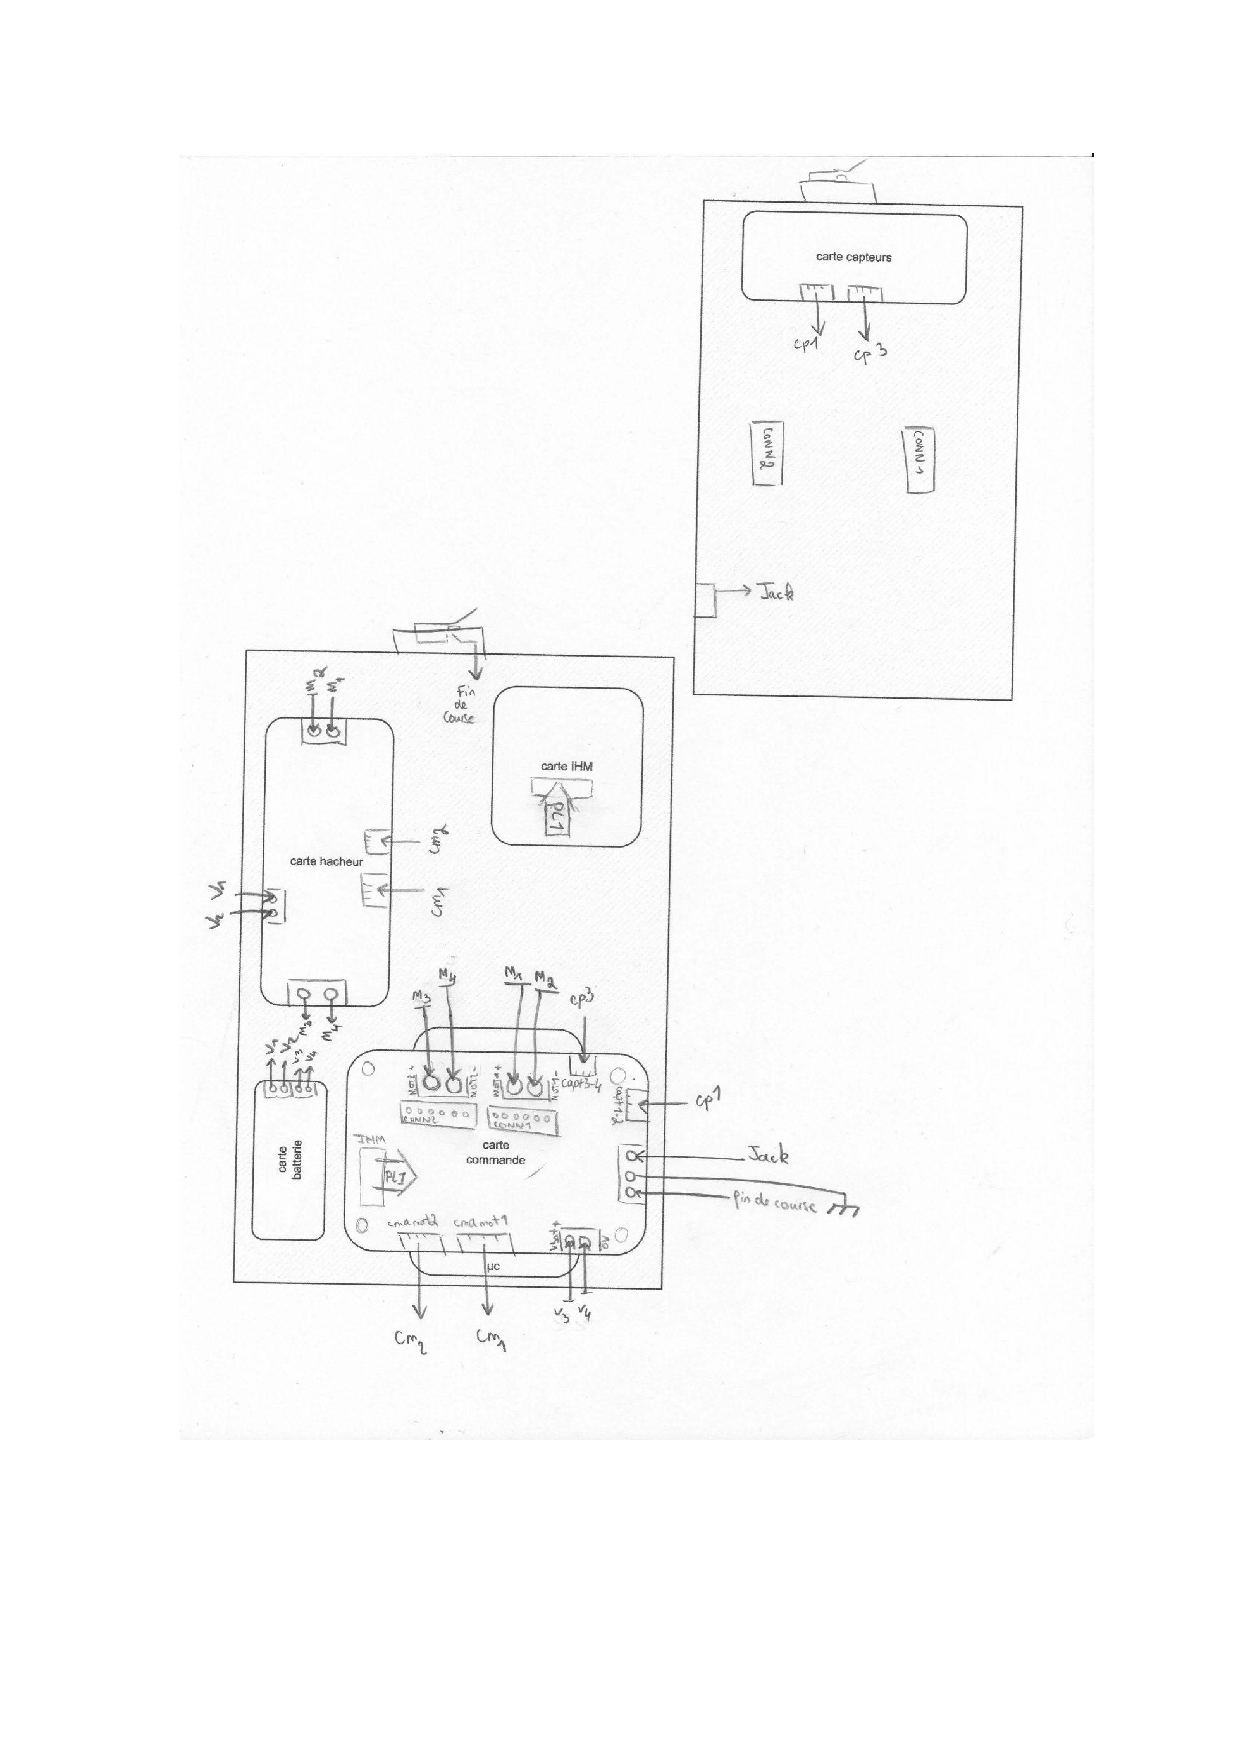
\includegraphics[width=1.5\linewidth]{pdf/cablages.pdf}}
  \captionof{figure}{\emph{Schéma de cablâge simplifié du robot}}
  \label{fig:schcablage}
\end{minipage}%
\end{figure}

\vfill
\noindent\makebox[\linewidth]{\rule{.8\paperwidth}{.6pt}}\\[0.2cm]
I.U.T. Nice Côte d'Azur - SAE Robot - 2023 \hfill goofyBot
\noindent\makebox[\linewidth]{\rule{.8\paperwidth}{.6pt}}
\newpage

\subsection{Électronique}

Afin que notre robot fonctionne, il faut qu'il soit alimenté, et que toute l'électronique fonctionne correctement.

Le robot reçoit en entrée sur la carte batterie une tension de 12V mais les cartes électroniques doivent être alimentées en 5V et en 3.3V pour fonctionner. 
Ainsi sur nos cartes il y a des composants actifs qui jouent des rôles importants.
Nous avons premièrement des régulateurs de tension qui sont sur la carte de commande et qui génèrent du 5V ou du 3.3V pour alimenter le microcontrôleur, et les différentes cartes électroniques.

\begin{figure}[H]
\centering
\begin{minipage}{.5\textwidth}
  \centering
  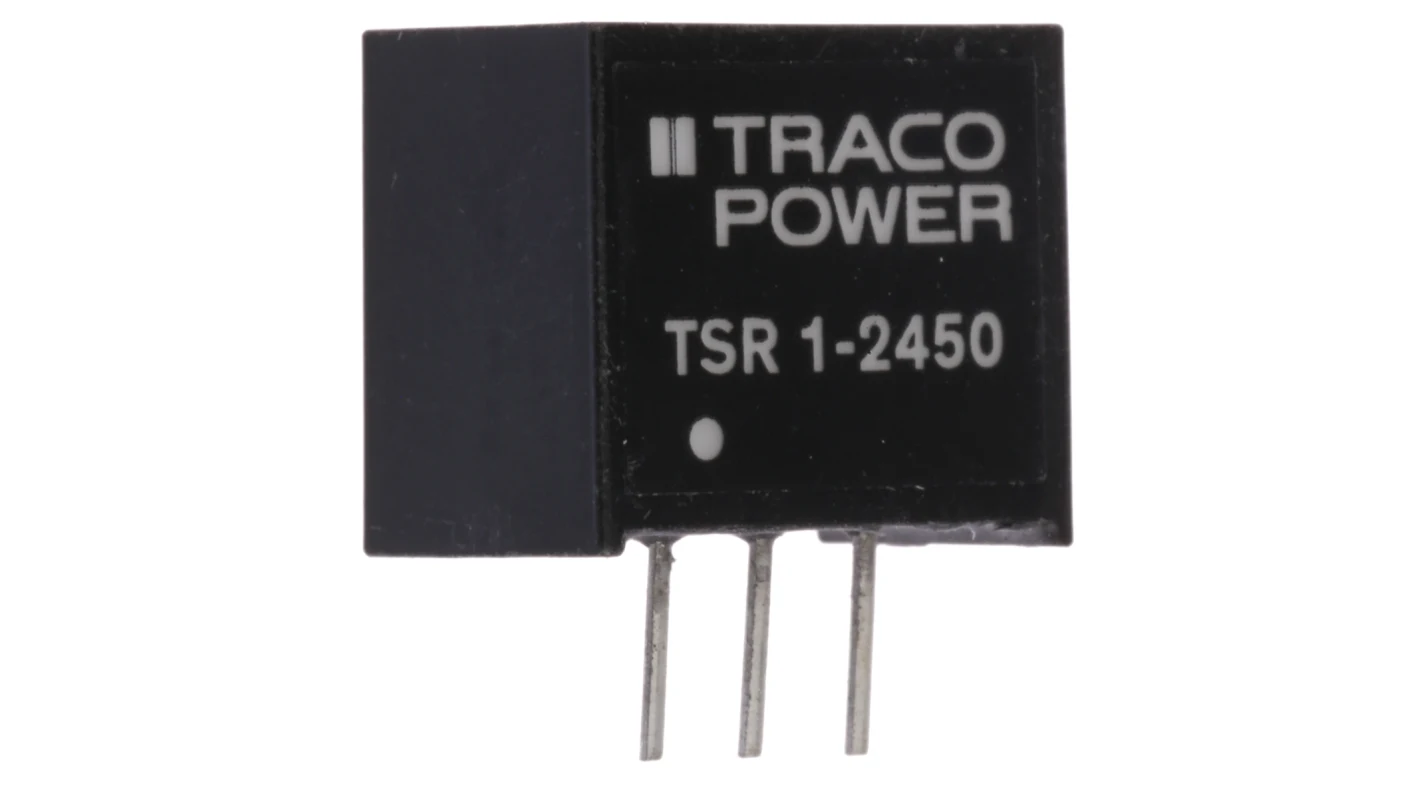
\includegraphics[width=.8\linewidth]{img/composants/tsr.png}
  \captionof{figure}{\emph{régulateur 12V à 5V}}
  \label{fig:tsr}
\end{minipage}%
\begin{minipage}{.5\textwidth}
  \centering
  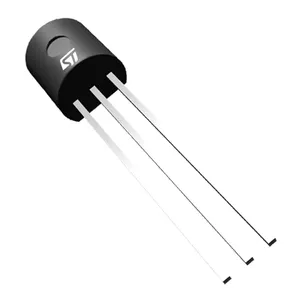
\includegraphics[width=.8\linewidth]{img/composants/l78l.png}
  \captionof{figure}{\emph{régulateur 5V à 3.3V}}
  \label{fig:l78l}
\end{minipage}
\end{figure}

Dans l’autre sens, nous avons des optocoupleurs à entrée inverseurs sur la carte commande qui servent à prendre la tension de sortie du microcontrôleur et la transformer en une tension de 12V à appliquer aux bornes du moteur, en faisant passer le courant 2 fois dedans pour récupérer le même signal mais augmenté.

Nous avons un capteur de fin de course qui est connecté sur la borne + au contact normalement ouvert et la borne - au commun du capteur. Le circuit est donc fermé lorsque le fin de course est activé et ainsi le capteur envoie une valeur analogique de 1 lorsqu'il est fermé.
Il nous a fallu aussi intégrer le concept de résistance de pull-up/pull-down. Dans un montage Pull-up il y a une résistance est appelée Pull-up lorsque elle est directement connectée a l'entrée d'alimentation et que lorsque le bouton poussoir est enfoncée son entrée est 0 en état actif. Et inversement, un montage Pull-down intégre une résistance de Pull-down qui est reliée a la masse et l'entrée logique quand le bouton est activé est 1.       

\vfill
\noindent\makebox[\linewidth]{\rule{.8\paperwidth}{.6pt}}\\[0.2cm]
I.U.T. Nice Côte d'Azur - SAE Robot - 2023 \hfill goofyBot
\noindent\makebox[\linewidth]{\rule{.8\paperwidth}{.6pt}}
\newpage

\begin{figure}[H]
\centering
\begin{minipage}{.5\textwidth}
  \centering
  \centerline{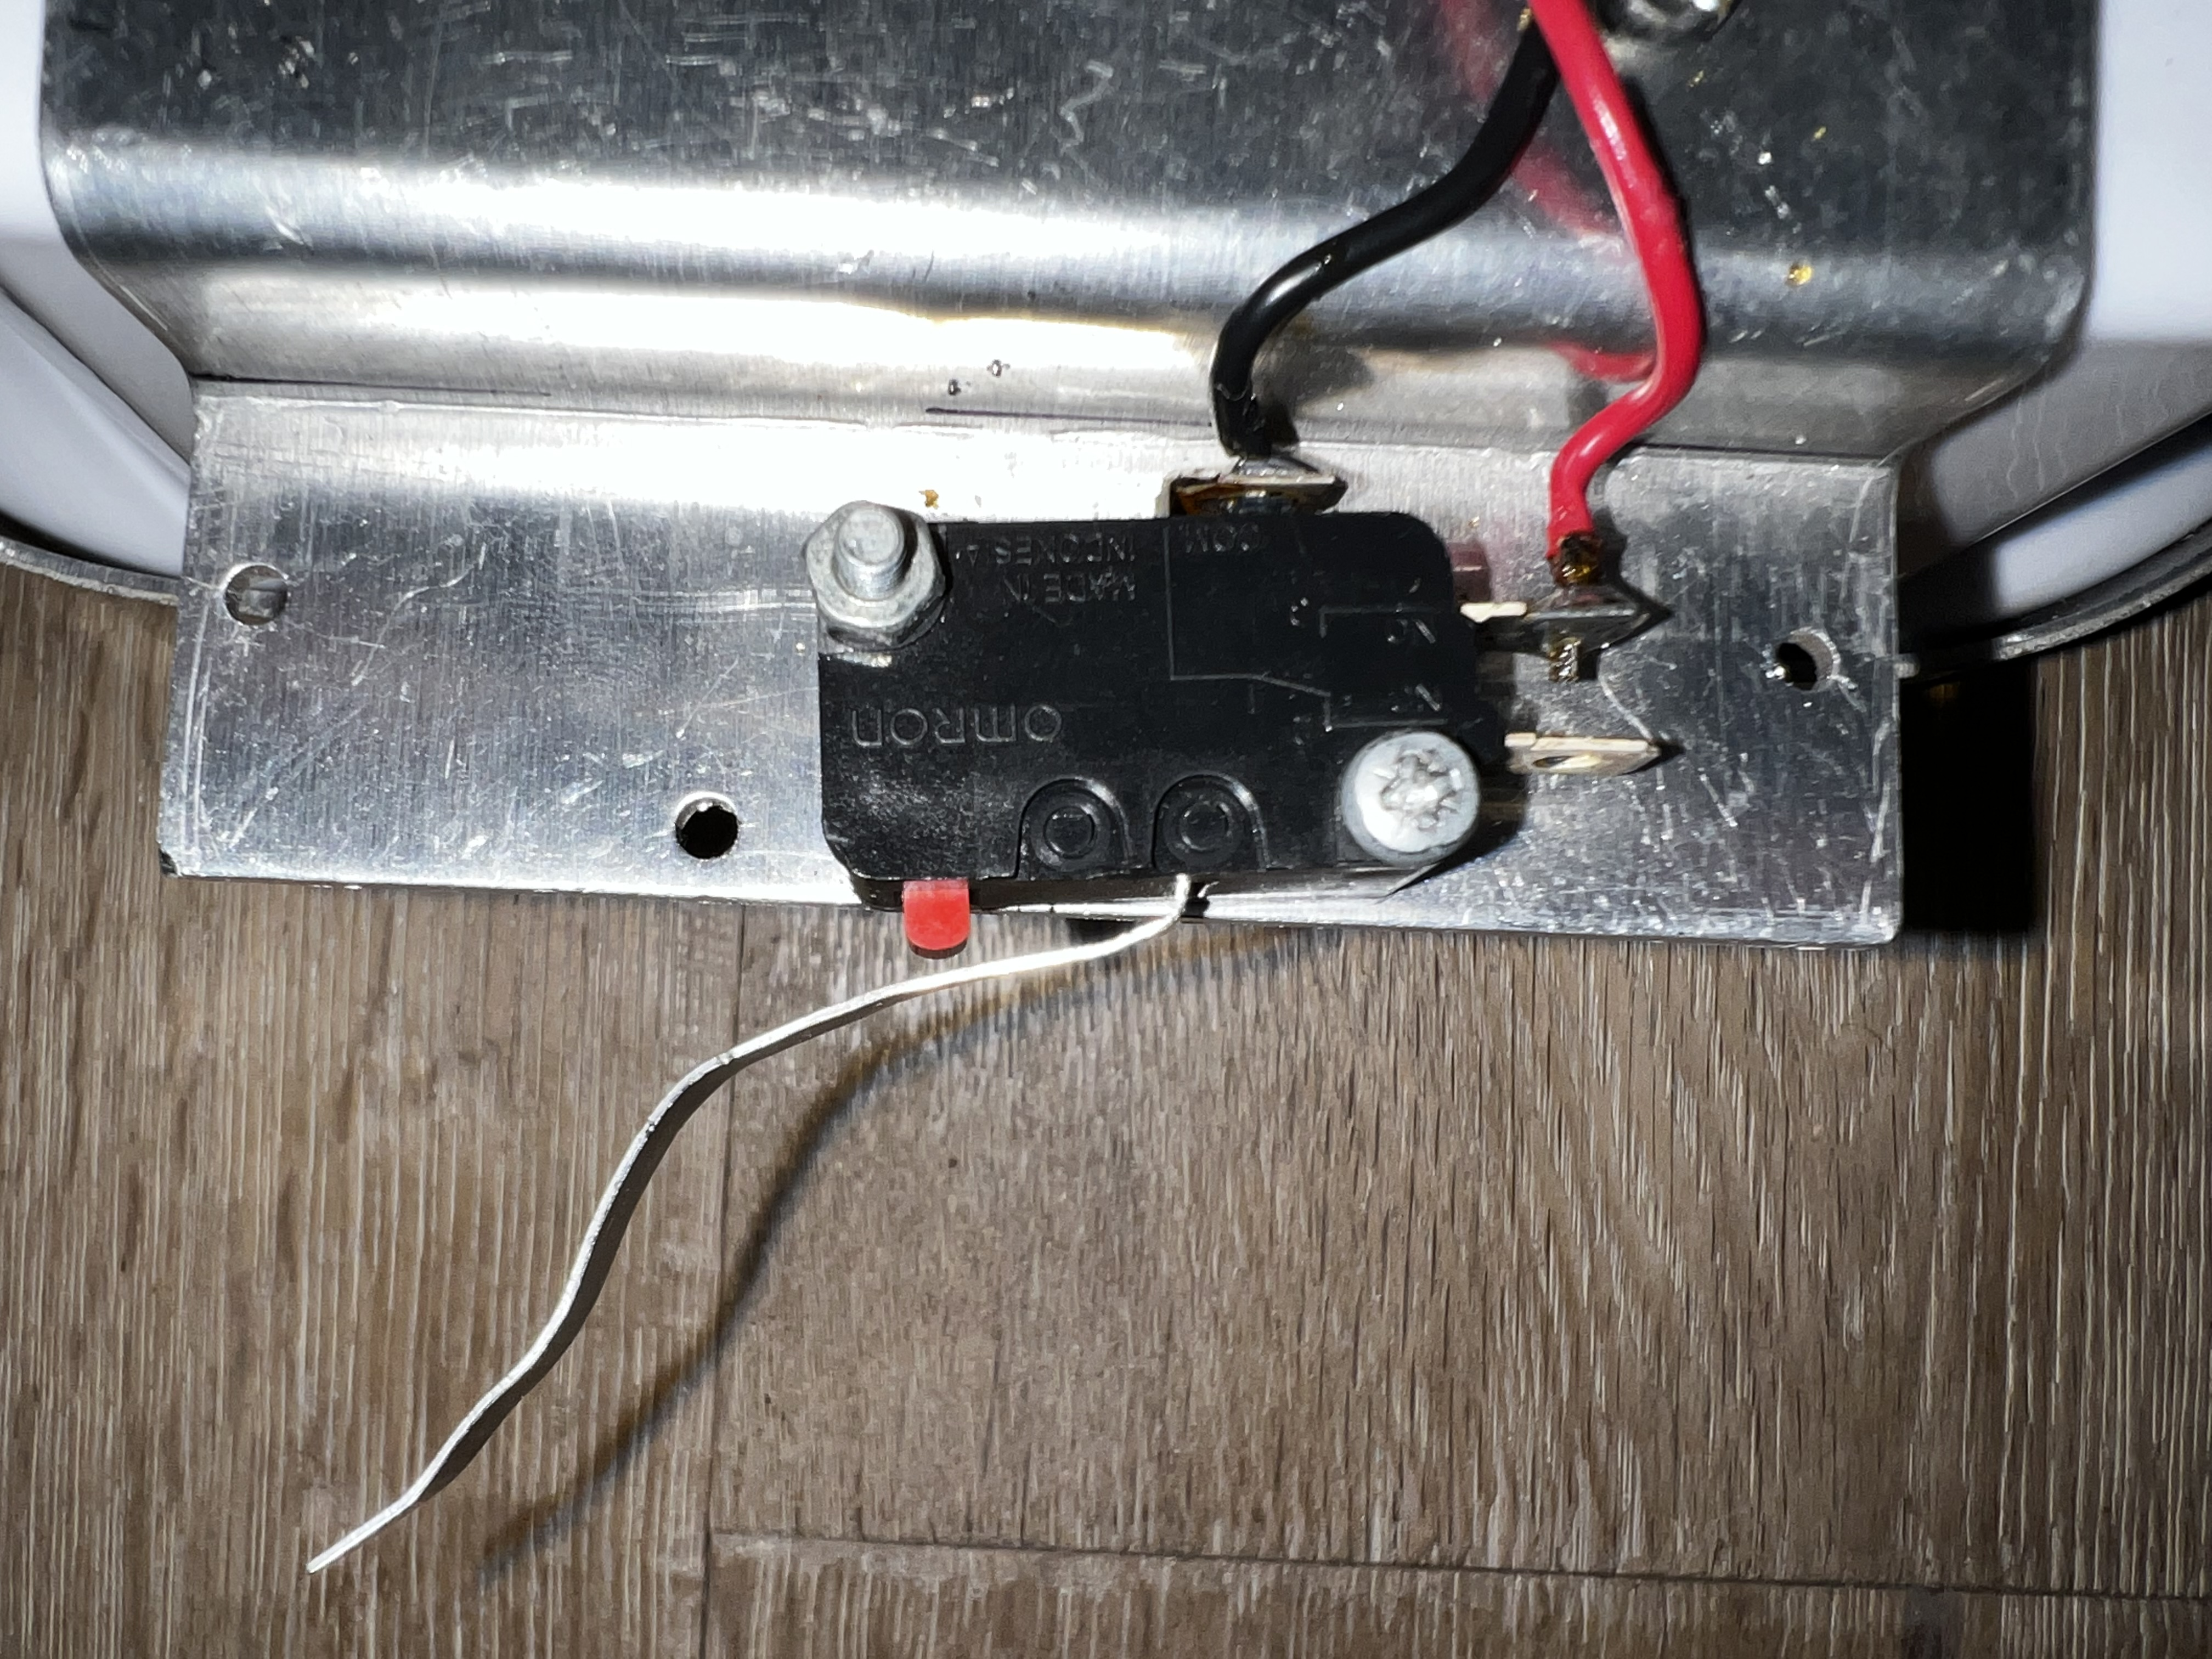
\includegraphics[width=1\linewidth]{img/cartes/tor.jpeg}}
  \captionof{figure}{\emph{capteur TOR Fin de Course}}
  \label{fig:tor}
\end{minipage}%
\end{figure}

\begin{figure}[H]
\centering
\begin{minipage}{.5\textwidth}
  \centering
  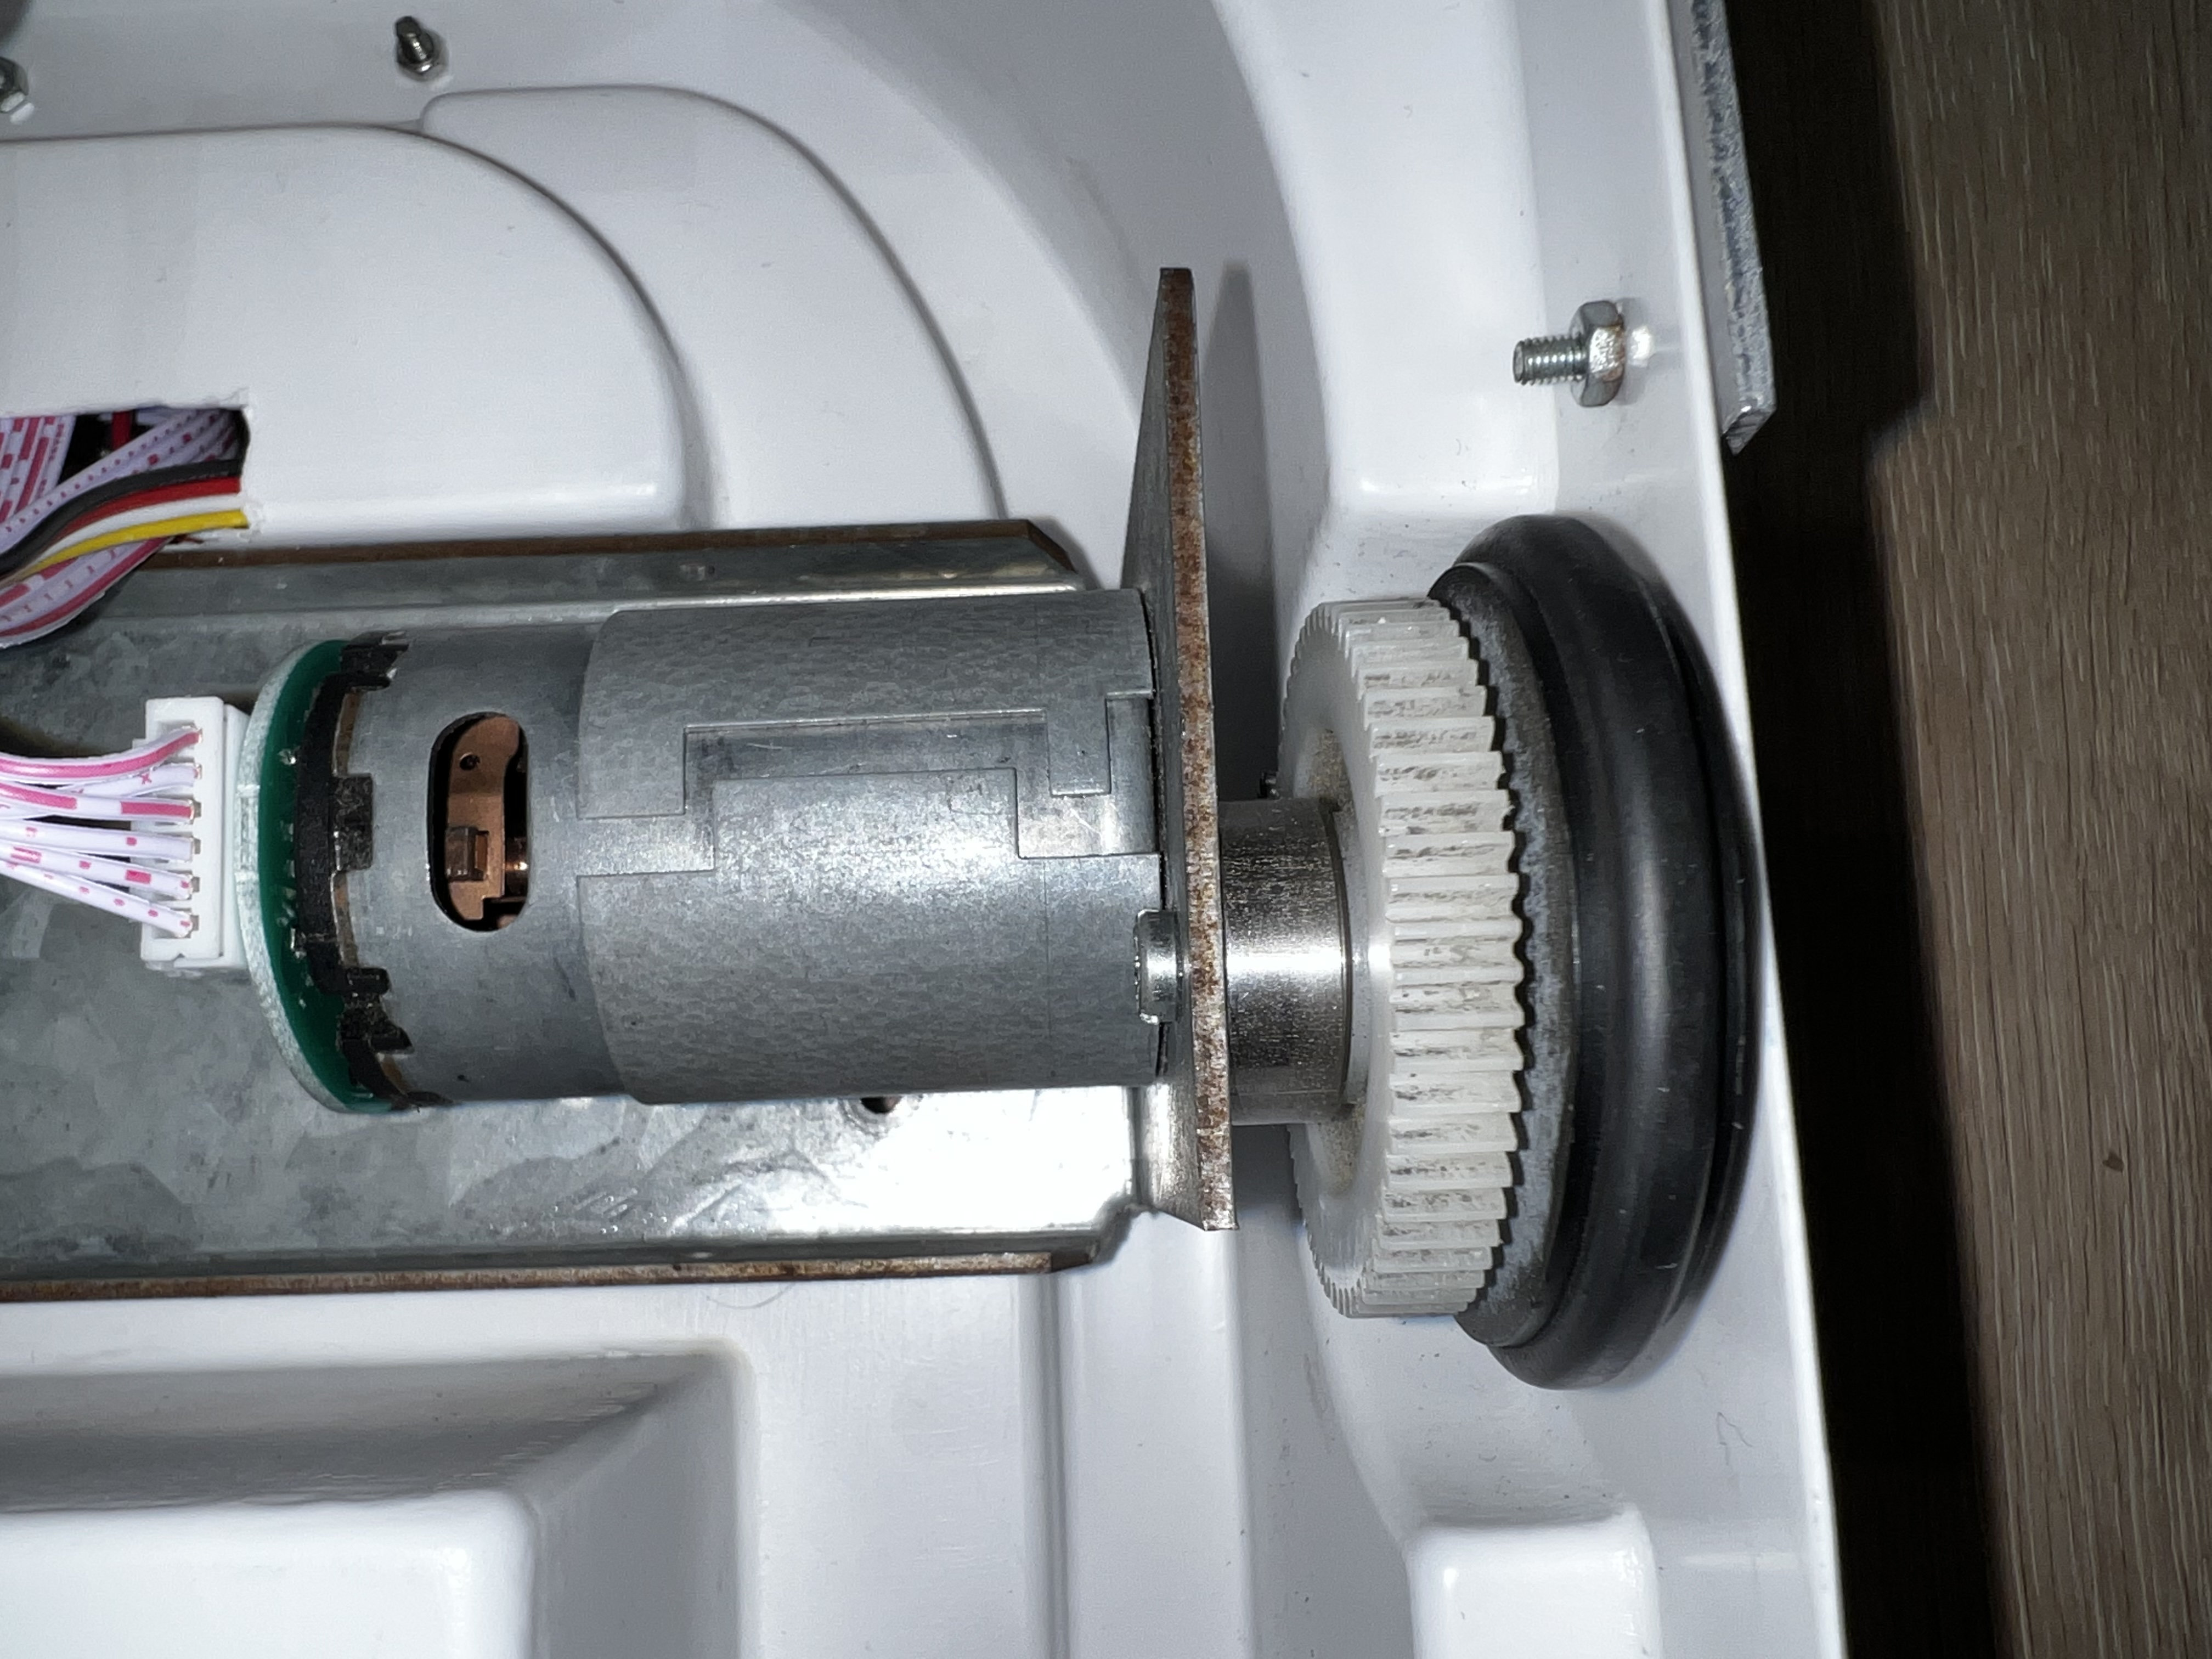
\includegraphics[width=.8\linewidth]{img/cartes/moteur.jpeg}
  \captionof{figure}{\emph{Roue + Moteur}}
  \label{fig:moteur}
\end{minipage}%
\begin{minipage}{.5\textwidth}
  \centering
  \includegraphics[width=.8\linewidth]{img/cartes/moteurs.jpeg}
  \captionof{figure}{\emph{Essieu}}
  \label{fig:essieu}
\end{minipage}
\end{figure}

\subsection{Cartes}
Pour mener à bien notre projet nous avons eu besoin de concevoir 3 cartes électroniques : la carte IHM, la carte capteurs et la carte hacheur. Pour cela nous avons dû utiliser le logiciel DesignSpark PCB, qui est un logiciel de conception de circuits imprimés (PCB) gratuit développé par RS Components, une entreprise de distribution de composants électroniques. 

\vfill
\noindent\makebox[\linewidth]{\rule{.8\paperwidth}{.6pt}}\\[0.2cm]
I.U.T. Nice Côte d'Azur - SAE Robot - 2023 \hfill goofyBot
\noindent\makebox[\linewidth]{\rule{.8\paperwidth}{.6pt}}
\newpage


Il permet aux utilisateurs de concevoir des schémas électriques, de créer des circuits imprimés et de générer des fichiers de fabrication pour la production de PCB.

\begin{figure}[H]
\centering
\begin{minipage}{.5\textwidth}
  \centering
  \centerline{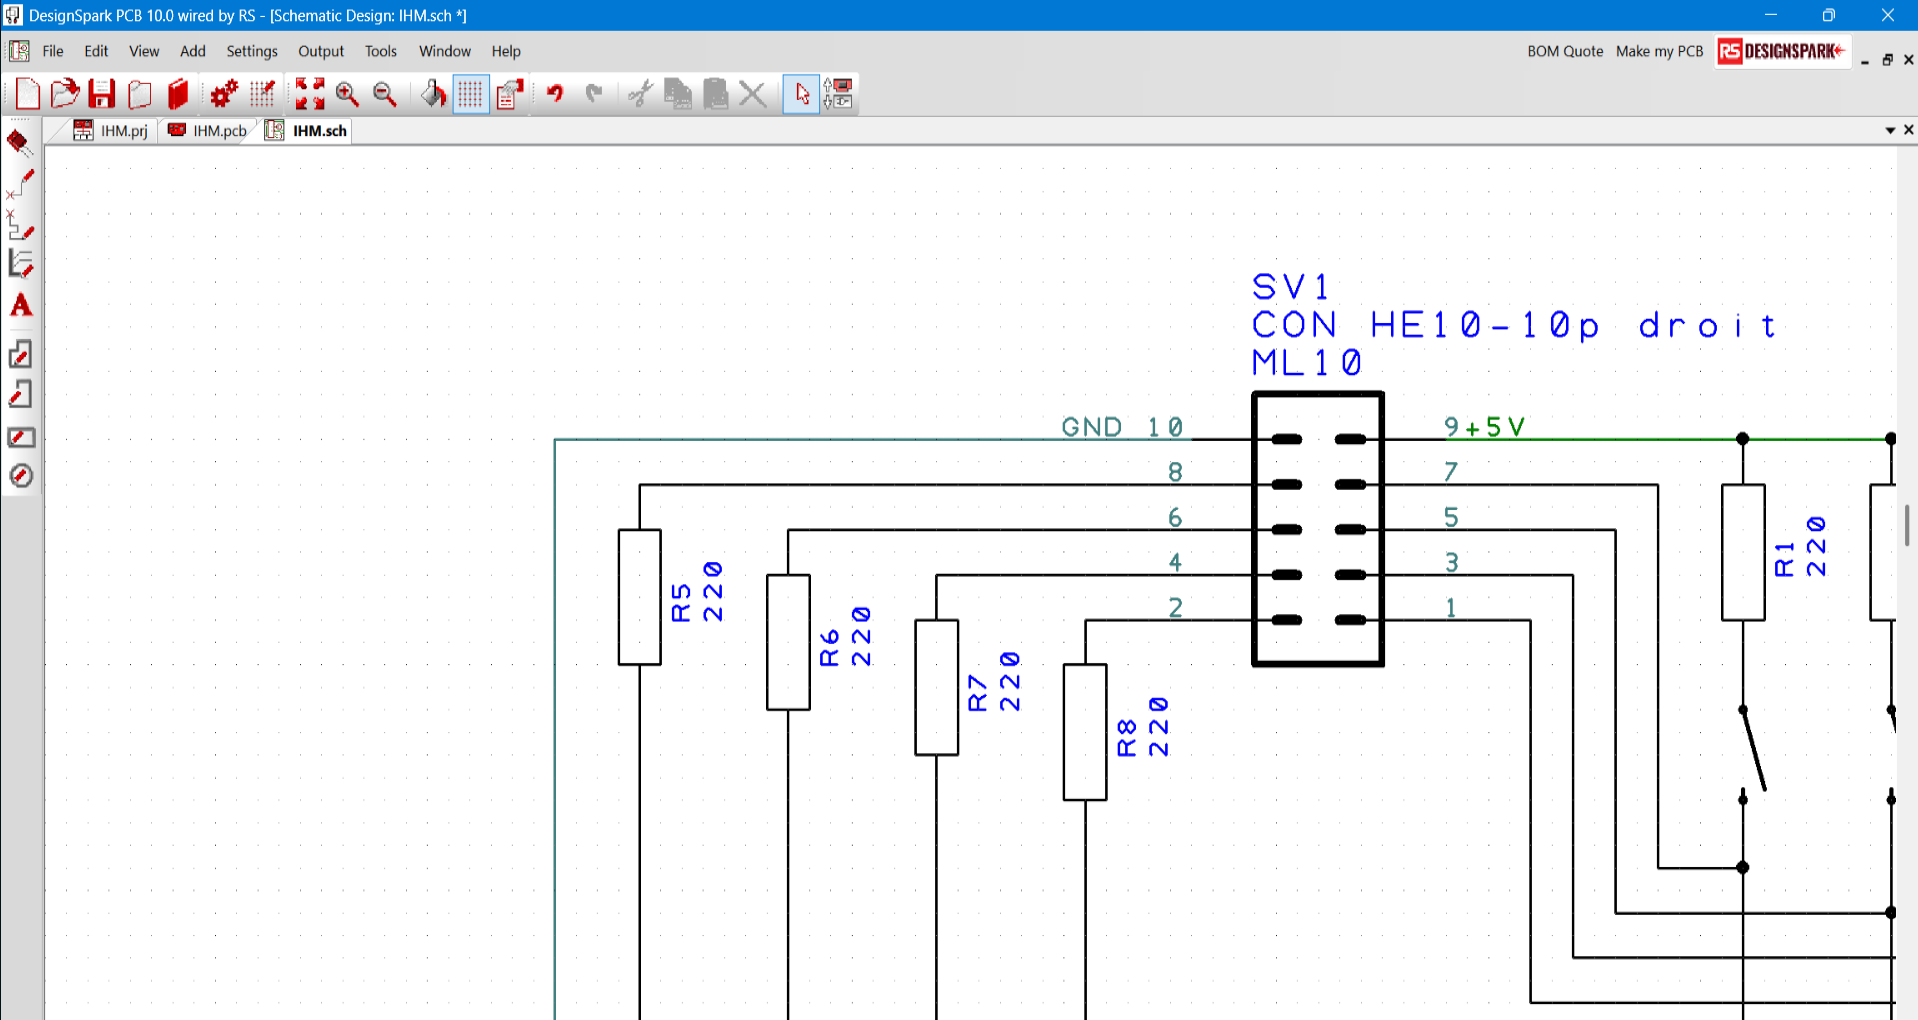
\includegraphics[width=1.5\linewidth]{img/dspcb.png}}
  \captionof{figure}{\emph{Interface utilisateur de DesignSpark PCB}}
  \label{fig:dspcb}
\end{minipage}%
\end{figure}

\subsubsection{Carte Batterie}

La carte batterie pour le projet est utilisée pour alimenter les différents composants du robot, tels que les moteurs, les capteurs et le microcontrôleur. 
L’objectif de cette carte est de contrôler la tension d’entrée d’alimentation du robot pour assurer un bon fonctionnement nominal et assurer que celui-ci ne s'arrête pas en pleine course.

Cette carte est composée premièrement par un comparateur de tension qui se base pour sa comparaison sur la tension d’une diode zener, réputée pour sa stabilité, et grâce à un pont diviseur,cette tension est comparée avec la tension d’entrée pour s'assurer que la batterie est chargée et délivre une tension de 12V. 
Une led de mise sous tension s’allume et si la tension est supérieure à 12V une led verte s’allume et si cette tension est inférieure à 12V elle ne s’allume pas.


Cette carte est composée aussi d’un shunt qui permet de vérifier que la comparaison est faite en mettant une tension de comparaison volontairement inférieure à 12V et un fusible qui protège les composants.
Sur le haut, il y a des connecteurs qui permettent d’alimenter les cartes commande et hacheur et un interrupteur qui permet de gérer l’alimentation du robot.

\vfill
\noindent\makebox[\linewidth]{\rule{.8\paperwidth}{.6pt}}\\[0.2cm]
I.U.T. Nice Côte d'Azur - SAE Robot - 2023 \hfill goofyBot
\noindent\makebox[\linewidth]{\rule{.8\paperwidth}{.6pt}}
\newpage

\begin{figure}[H]
\centering
\begin{minipage}{.3\textwidth}
  \centering
  \centerline{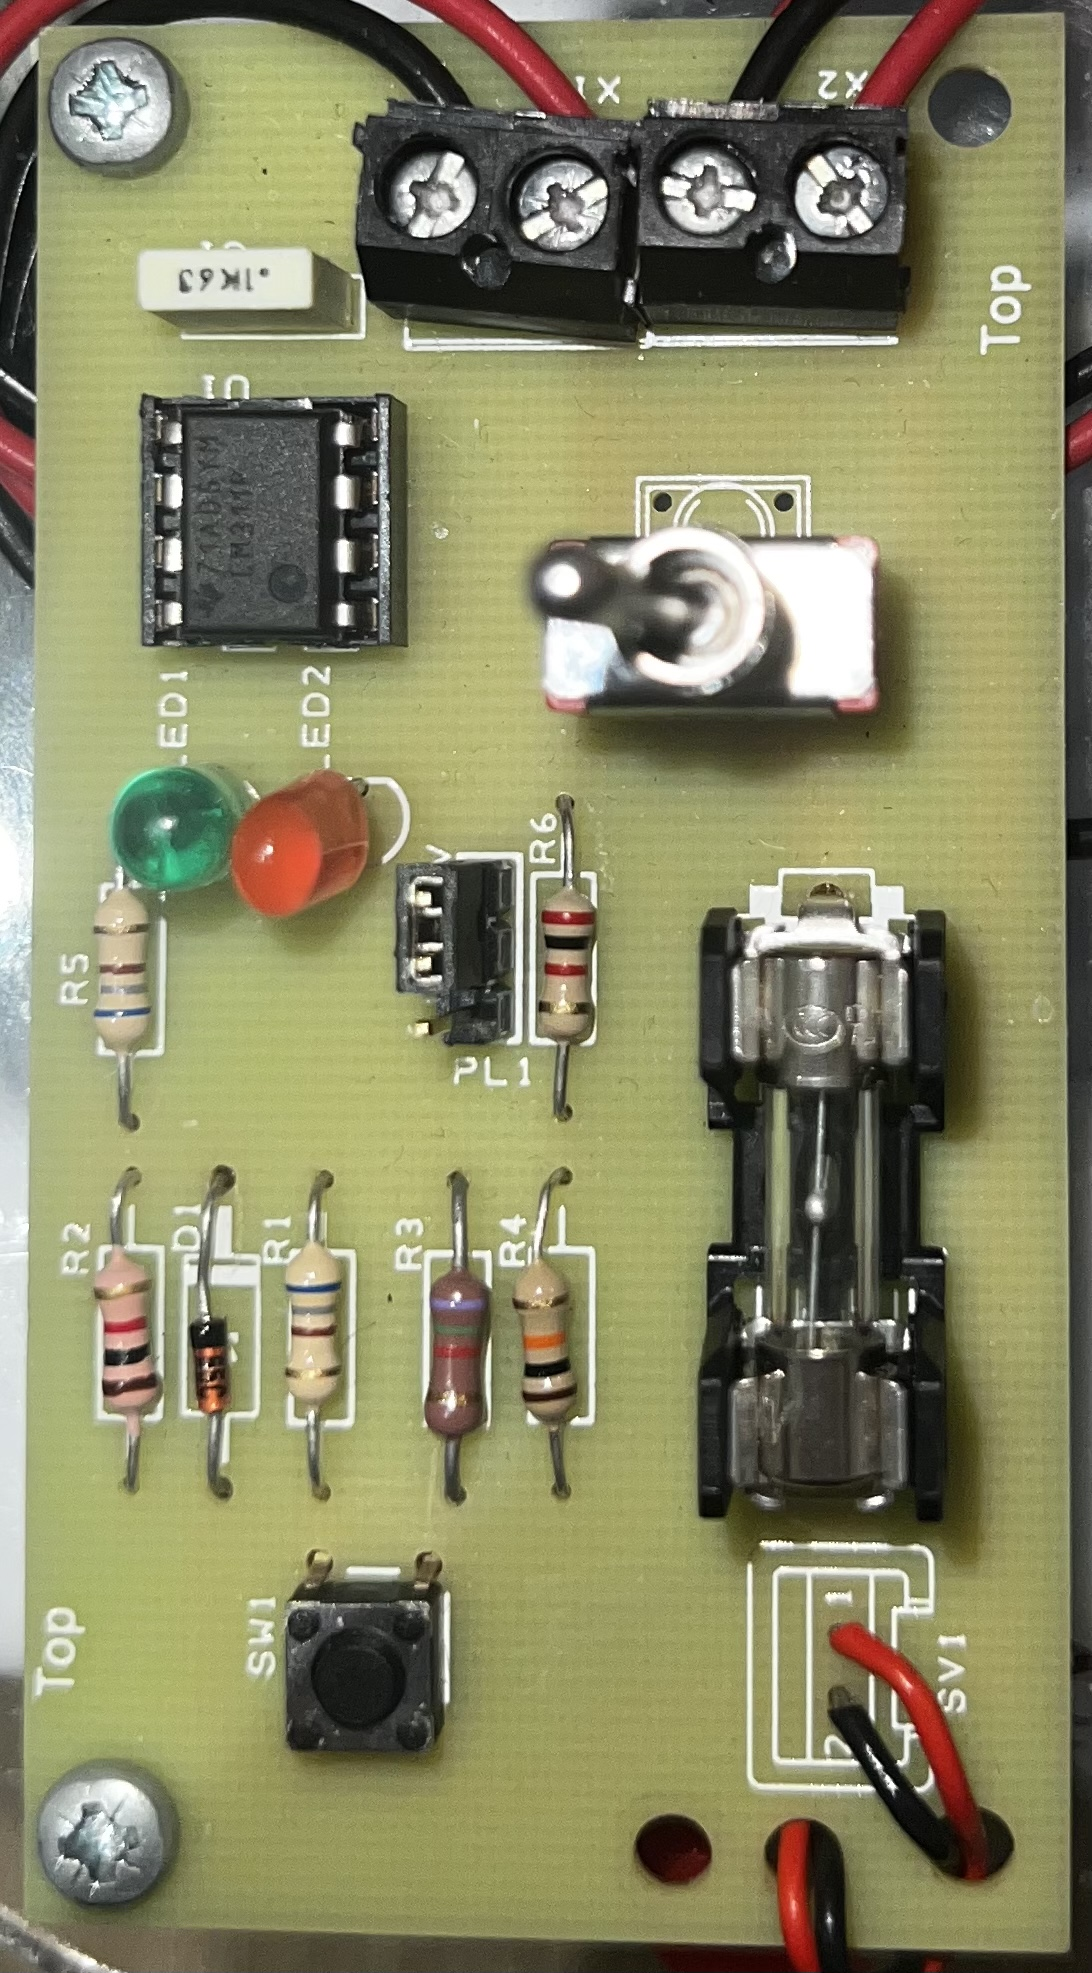
\includegraphics[width=1\linewidth, angle = -90]{img/cartes/batterie.jpeg}}
  \captionof{figure}{\emph{Carte Batterie}}
  \label{fig:batterie}
\end{minipage}%
\end{figure}

\vfill
\noindent\makebox[\linewidth]{\rule{.8\paperwidth}{.6pt}}\\[0.2cm]
I.U.T. Nice Côte d'Azur - SAE Robot - 2023 \hfill goofyBot
\noindent\makebox[\linewidth]{\rule{.8\paperwidth}{.6pt}}
\newpage


\subsubsection{Carte IHM}

La carte IHM (Interface Homme-Machine) est un élément clé de notre projet. Elle a pour rôle de 
permettre à l'utilisateur de contrôler et de visualiser l'état du système de manière intuitive.
La carte IHM est principalement constituée de boutons poussoirs et de LEDs. Elle est connectée au microcontrôleur via une interface de communication (la carte commande), qui lui permet de recevoir des informations et de transmettre des commandes.

Les boutons poussoirs sont des interrupteurs à bascule qui sont actionnés par une pression sur leur surface. Ils peuvent être utilisés pour lancer une action ou basculer entre différents états. 

Dans le cas de la SAE, ils seront utilisés pour sélectionner le programme ou choisir des valeurs.
Les LEDs sont des composants électroniques qui émettent de la lumière lorsqu'ils sont alimentés par du courant électrique. Elles peuvent être utilisées pour indiquer l'état d'un système, en affichant une couleur différente en fonction de l'état.

\begin{figure}[H]
\centering
\begin{minipage}{.5\textwidth}
  \centering
  \centerline{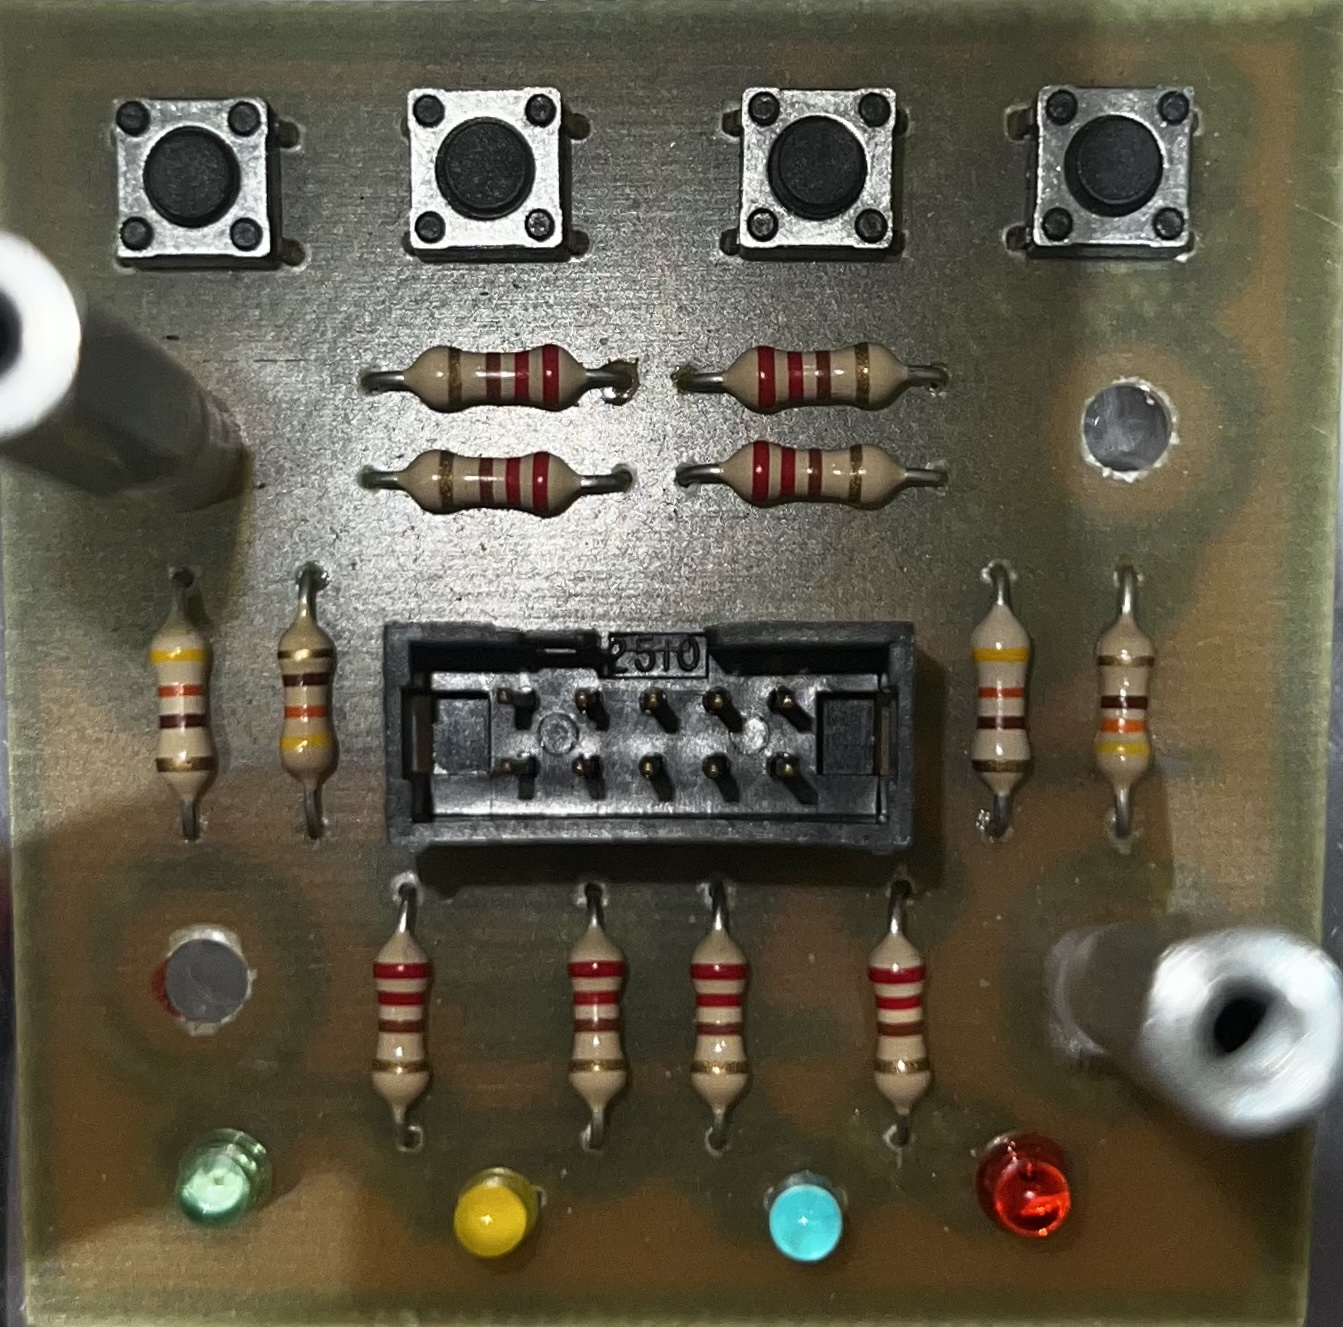
\includegraphics[width=1\linewidth]{img/cartes/ihm.jpeg}}
  \captionof{figure}{\emph{carte IHM}}
  \label{fig:ihm}
\end{minipage}%
\end{figure}

\vfill
\noindent\makebox[\linewidth]{\rule{.8\paperwidth}{.6pt}}\\[0.2cm]
I.U.T. Nice Côte d'Azur - SAE Robot - 2023 \hfill goofyBot
\noindent\makebox[\linewidth]{\rule{.8\paperwidth}{.6pt}}
\newpage

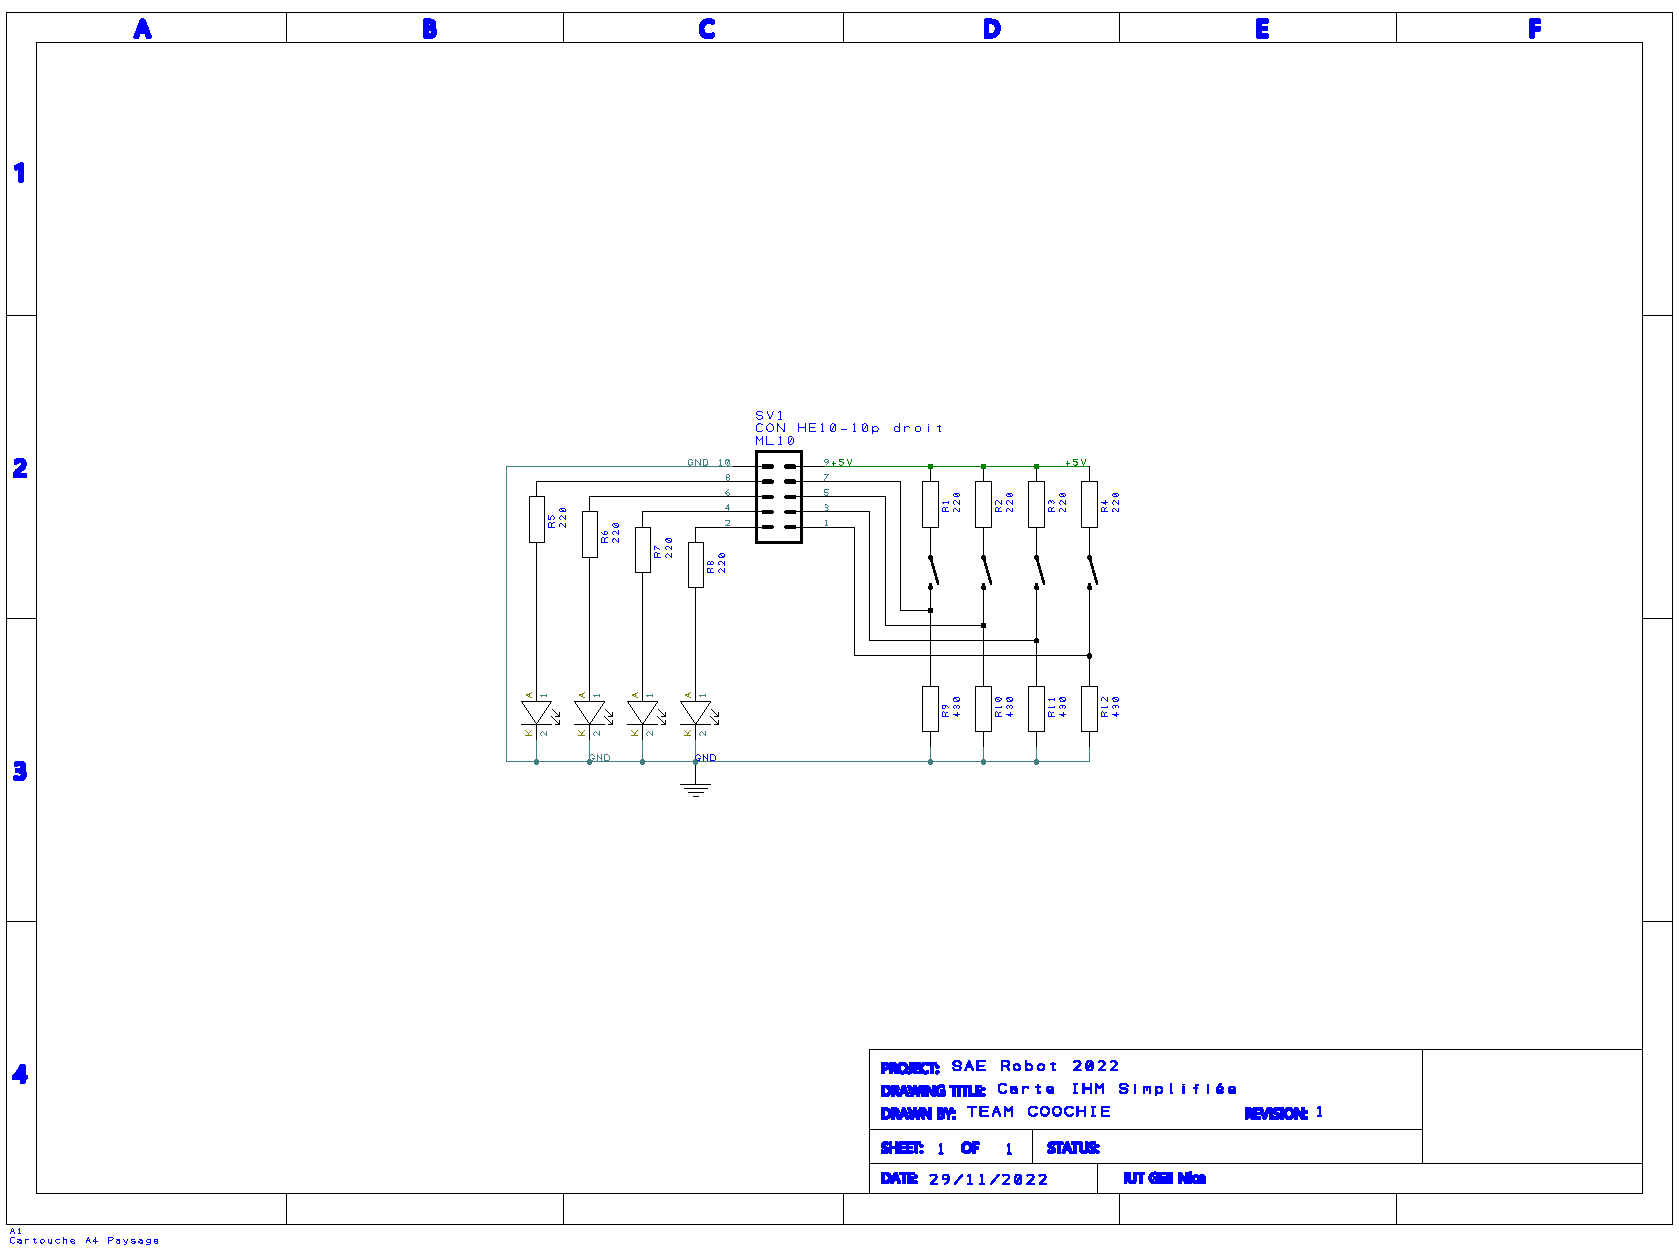
\includepdf[pages=-]{pdf/cartes/ihm/IHM - Project.pdf}
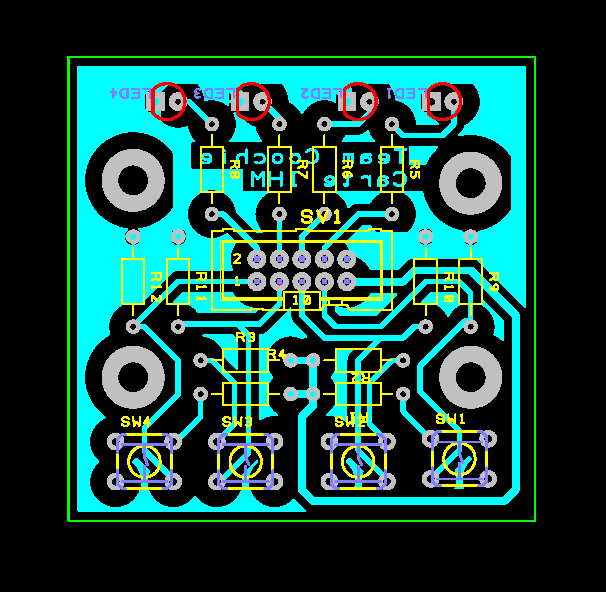
\includepdf[pages=-]{pdf/cartes/ihm/IHM - PCB.pdf}

\subsubsection{Carte Capteurs}

La carte capteur est une carte qui a pour objectif de détecter la ligne blanche pour diriger le robot.
Elle est composée de 4 capteurs TCRT5000L faits de phototransistors qui ont la particularité de laisser passer le courant quand son signal infrarouge envoyé est capté, c’est a dire lorsque il est au-dessus d’une surface blanche.

\begin{figure}[H]
\centering
\begin{minipage}{.5\textwidth}
  \centering
  \centerline{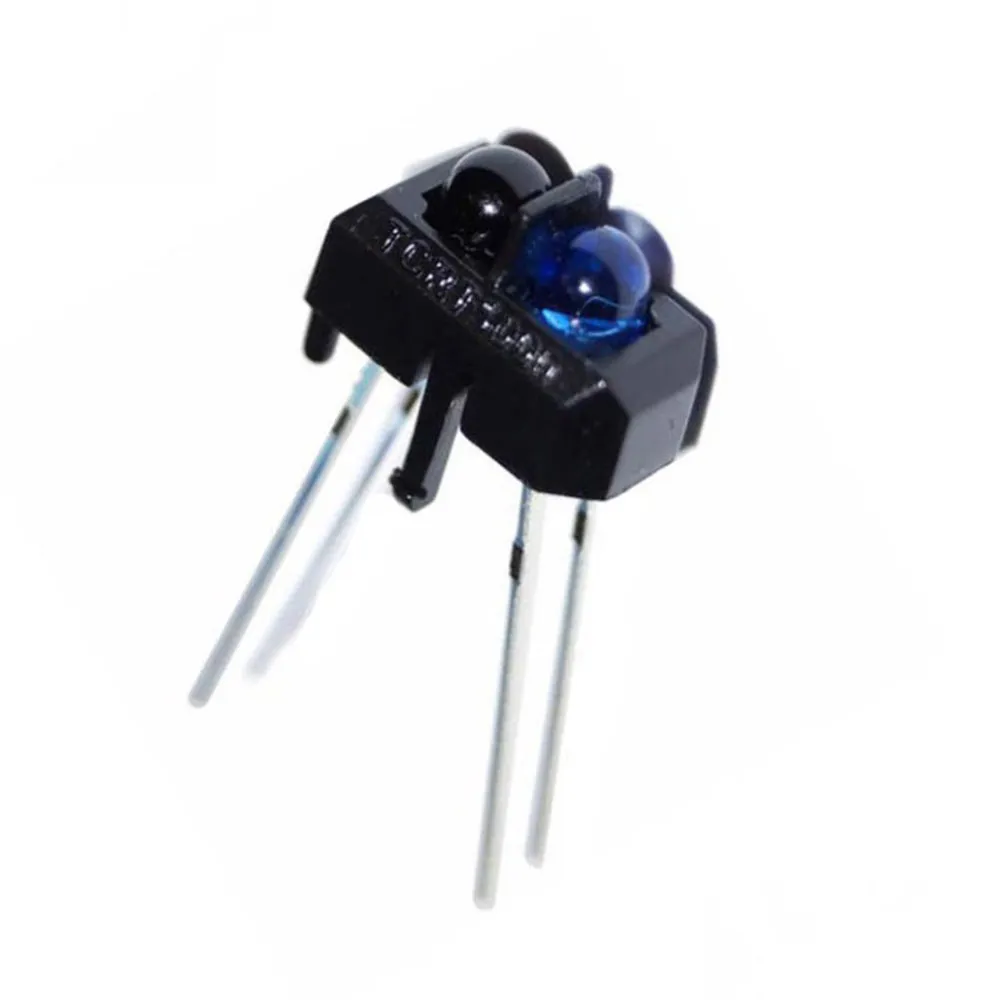
\includegraphics[width=0.6\linewidth]{img/composants/tcrt5000.png}}
  \captionof{figure}{\emph{Capteur TCRT5000}}
  \label{fig:tcrt5000}
\end{minipage}%
\end{figure}
Nous avons choisi ces derniers pour leur épaisseur plutôt négligeable et car nous avions réalisé des études préliminaires dessus et avons conclu que la différence de potentiel entre une surface blanche ou noire était la plus significative.

Parmi les quatre capteurs, deux sont en permanence sur la ligne a 19 mm de distance pour s'assurer de rester centré sur la ligne et se re-guider sur la ligne dans le cas où un des deux capteurs détectent une déviation de trajectoire jusqu'à ce que la ligne soit retrouvée.


Les deux autres sont aux plus aux extrémités du robot, comme des capteurs d’urgence pour plusieurs raisons : identifier un espacement pour comprendre que le robot traverse les confettis, pour détecter la ligne dans le cas ou le robot perdrait le signal des deux capteurs centraux, pour encore une fois se redresser et de nouveau recevoir un signal de ligne blanche au centre et aussi pour identifier les raccourcis disponibles sur le circuit quand l’un d’eux est aperçu.


Ainsi dans l’épreuve des confettis tant que les quatre capteurs n’ont pas détecté une zone blanche le robot va tout droit et dans l’épreuve du suivi de ligne, nous suivons une machine à état précise qui nous permet d’aller jusqu'à la fin du parcours avec les capteurs servant donc à garder le robot sur la ligne.


Sur le PCB nous voyons les capteurs branchés chacun à deux résistances en série pour fixer le courant qui circule et le transformer en une tension mesurable.
Notre carte capteurs est désignée particulièrement dans notre équipe car nous avons choisi ce design pensant que le capteur serait plus performant pour re-capter la ligne dans les cas extrêmes.

\vfill
\noindent\makebox[\linewidth]{\rule{.8\paperwidth}{.6pt}}\\[0.2cm]
I.U.T. Nice Côte d'Azur - SAE Robot - 2023 \hfill goofyBot
\noindent\makebox[\linewidth]{\rule{.8\paperwidth}{.6pt}}
\newpage

Les capteurs sont reliés à la carte de commande qui enverra les données des capteurs au microcontrôleur qui traitera les informations pour agir sur le mouvement du robot par le biais de la carte hacheur.

\begin{figure}[H]
\centering
\begin{minipage}{.5\textwidth}
  \centering
  \centerline{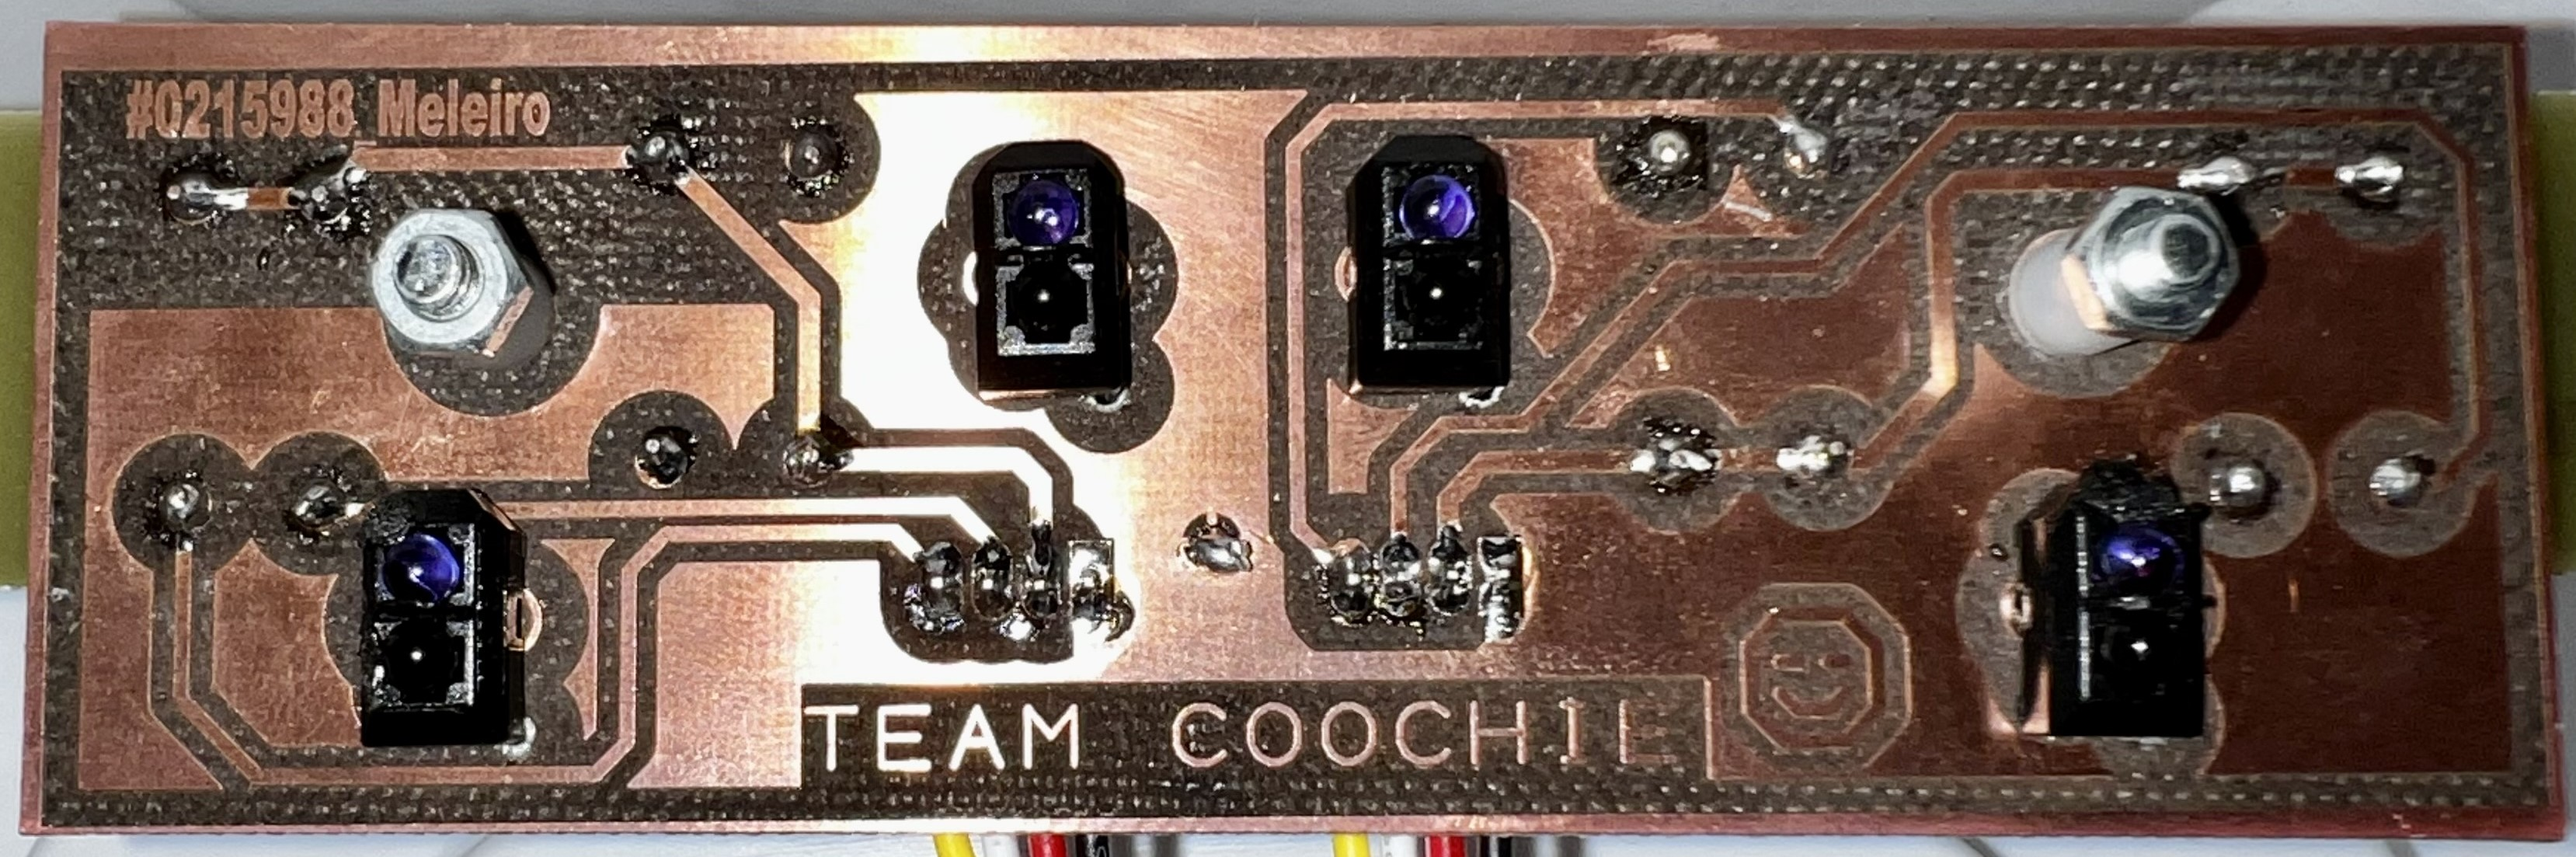
\includegraphics[width=1.5\linewidth]{img/cartes/capteur.jpeg}}
  \captionof{figure}{\emph{Carte 4 capteurs}}
  \label{fig:cartecapteurs}
\end{minipage}%
\end{figure}

\vfill
\noindent\makebox[\linewidth]{\rule{.8\paperwidth}{.6pt}}\\[0.2cm]
I.U.T. Nice Côte d'Azur - SAE Robot - 2023 \hfill goofyBot
\noindent\makebox[\linewidth]{\rule{.8\paperwidth}{.6pt}}
\newpage

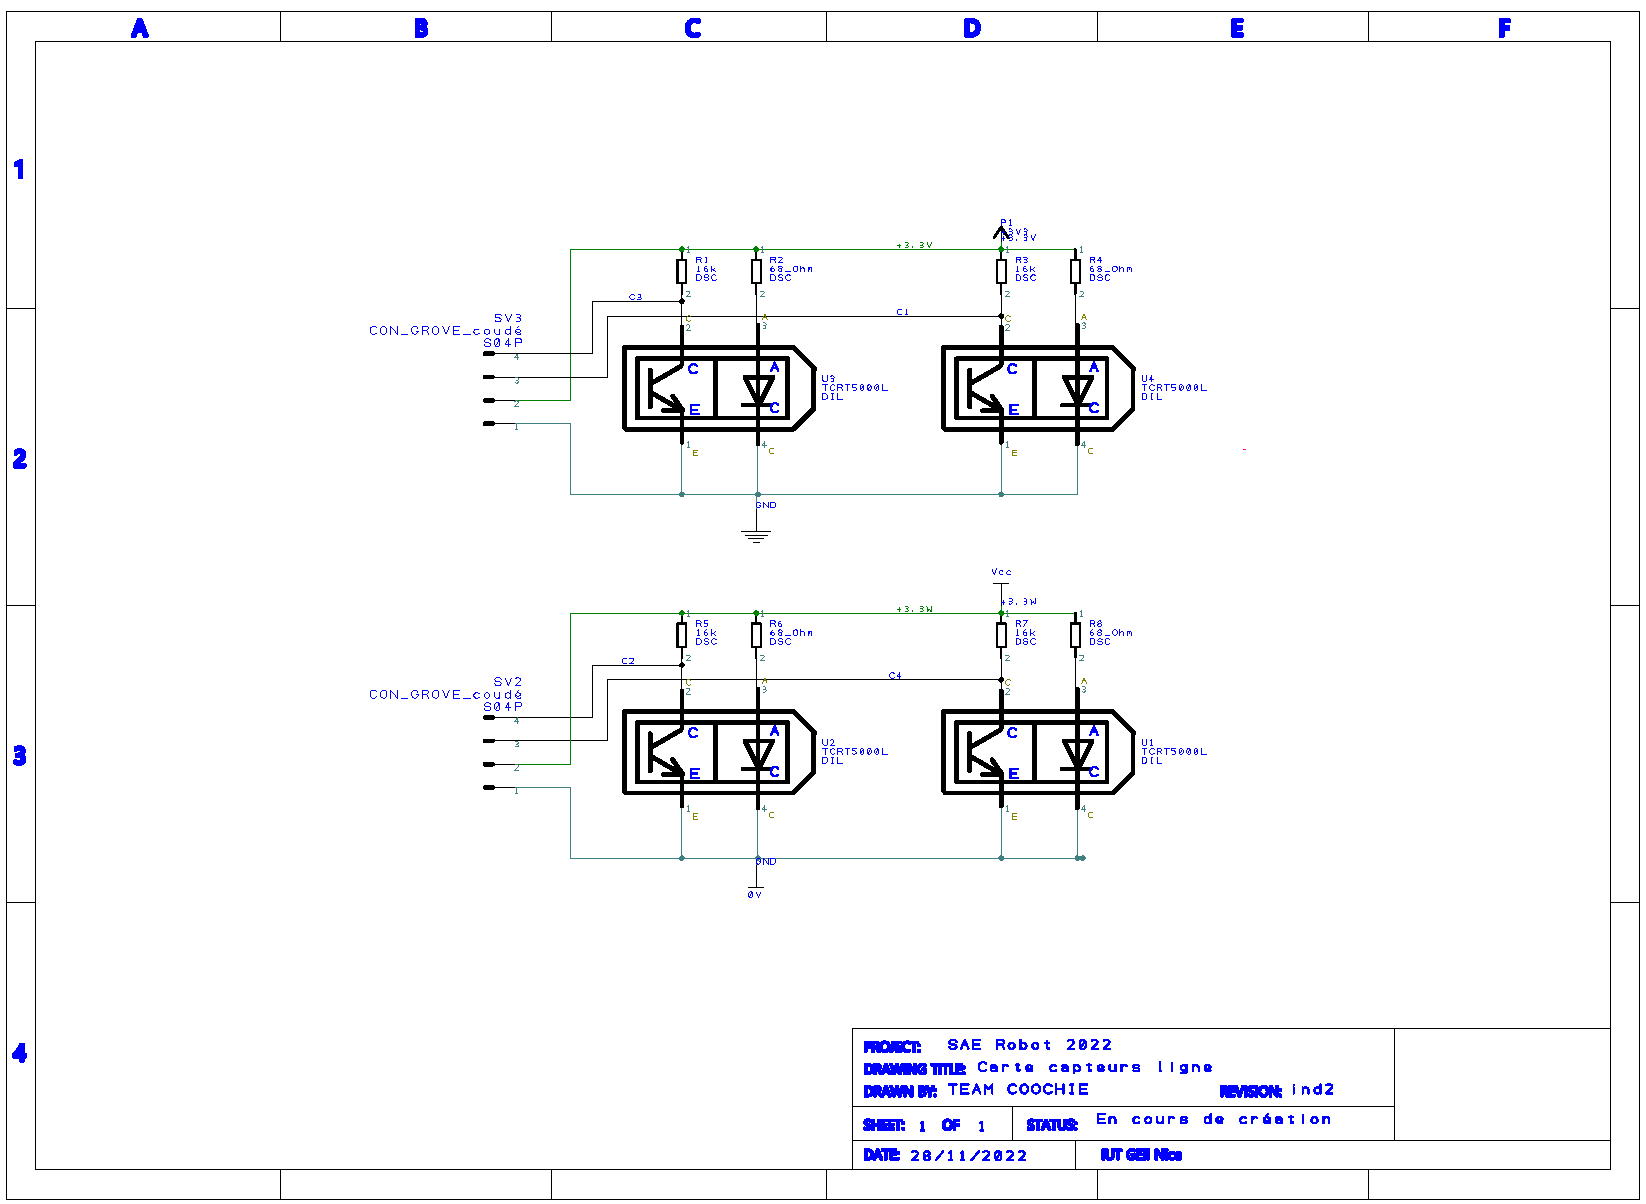
\includepdf[pages=-]{pdf/cartes/capteurs/CartesCapteurs - Project.pdf}

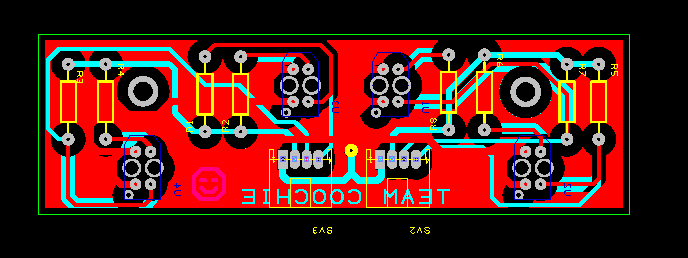
\includepdf[pages=-]{pdf/cartes/capteurs/CartesCapteurs - PCB.pdf}

\subsubsection{Carte Hacheur}
La carte hacheur est une carte qui doit gérer la vitesse des moteurs dans l’optique de contrôler les déplacements du robot car pour répondre au cahier des charges nous devons pouvoir faire varier la vitesse des moteurs et leur sens.


L’objectif de la carte est d’obtenir une tension de sortie variable pour nous permettre le contrôle des moteurs dans les 4 quadrants afin de pouvoir accélérer et freiner dans les 2 sens qui sont avant et arrière.


Nous avons trouvé en séance de projet tuteuré la solution pour contrôler les moteurs et c’est le composant L298 qui sera intégré à notre carte.
Il est constitué de 2 ponts-H avec chacun 2 transistors servant à amplifier la tension pour délivrer du 12V aux bornes de 2 moteurs et aussi à changer le sens de rotation des moteurs en inversant le sens de courant qui les traverse.
On peut ainsi faire varier la vitesse des moteurs avec le micro-contrôleur en faisant varier l’entrée logique rapport cyclique de chacun et ainsi faire rouler le robot à la vitesse souhaitée ou le faire tourner.
Avec ses entrées de sens et de PWM pour chaque moteur, il prend donc place au milieu de notre carte électronique de contrôle intégral des moteurs du robot.


Nous voyons donc qu’en plus du composant nous avons des diodes de roue libre pour protéger les transistors et des condensateurs utilisés comme filtres passifs qui servent à lisser la tension d’entrée et la stabiliser.


\begin{figure}[H]
\centering
\begin{minipage}{.5\textwidth}
  \centering
  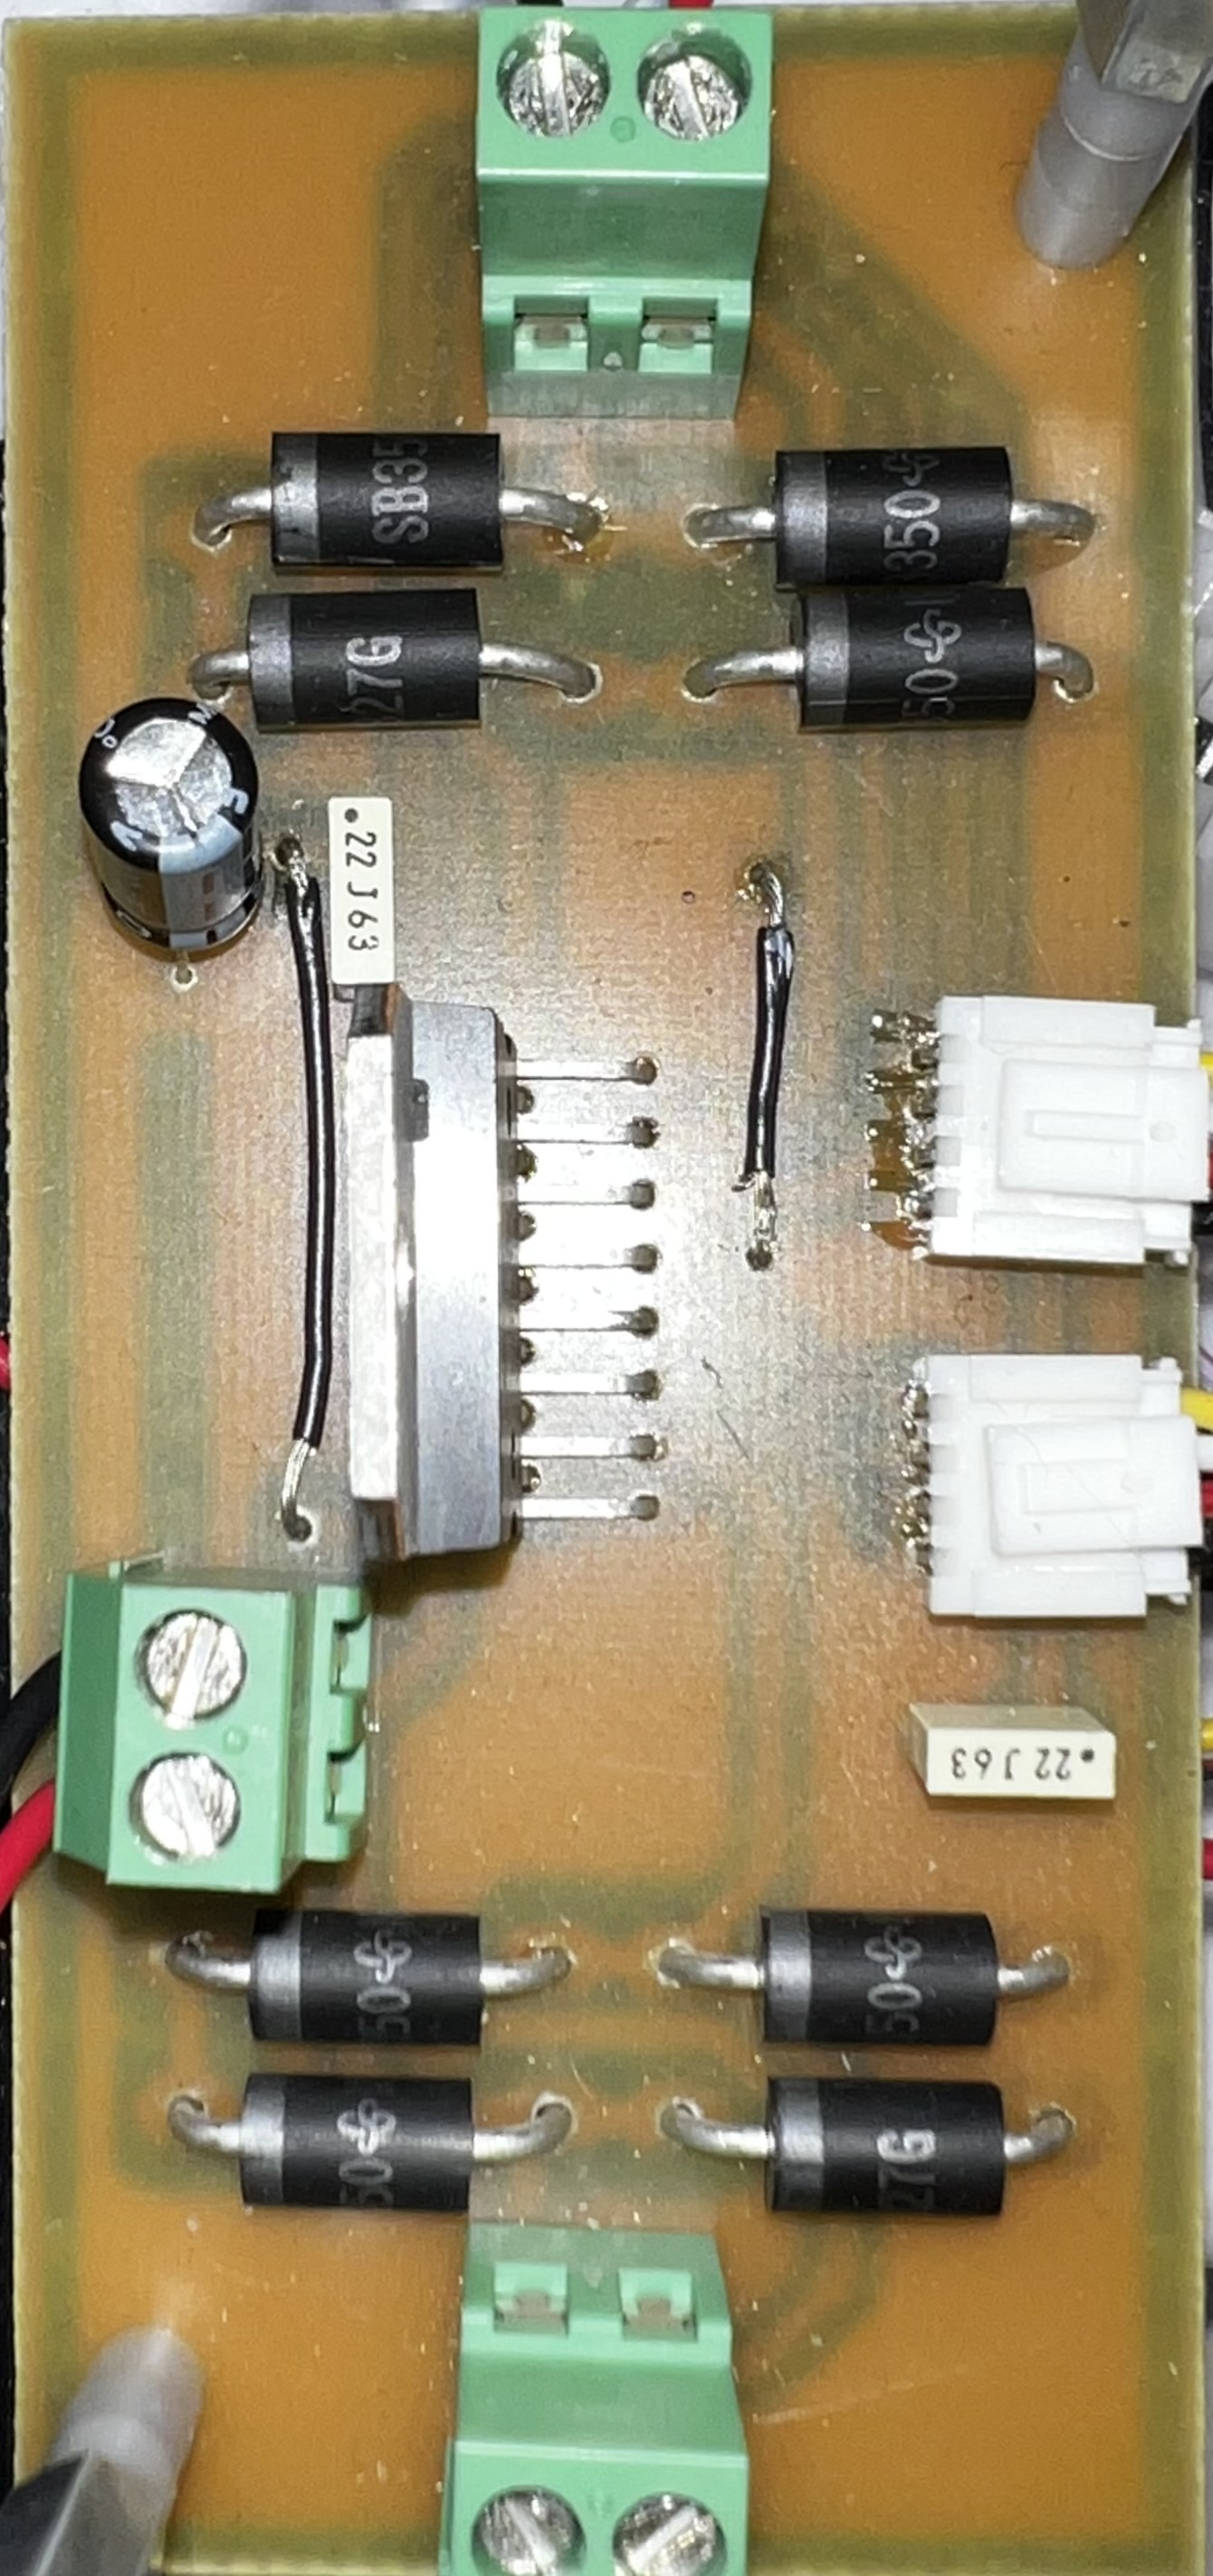
\includegraphics[width=.6\linewidth, angle = -90]{img/cartes/hacheur.jpeg}
  \captionof{figure}{\emph{Carte Hacheur}}
  \label{fig:hacheur}
\end{minipage}
\end{figure}

\vfill
\noindent\makebox[\linewidth]{\rule{.8\paperwidth}{.6pt}}\\[0.2cm]
I.U.T. Nice Côte d'Azur - SAE Robot - 2023 \hfill goofyBot
\noindent\makebox[\linewidth]{\rule{.8\paperwidth}{.6pt}}
\newpage

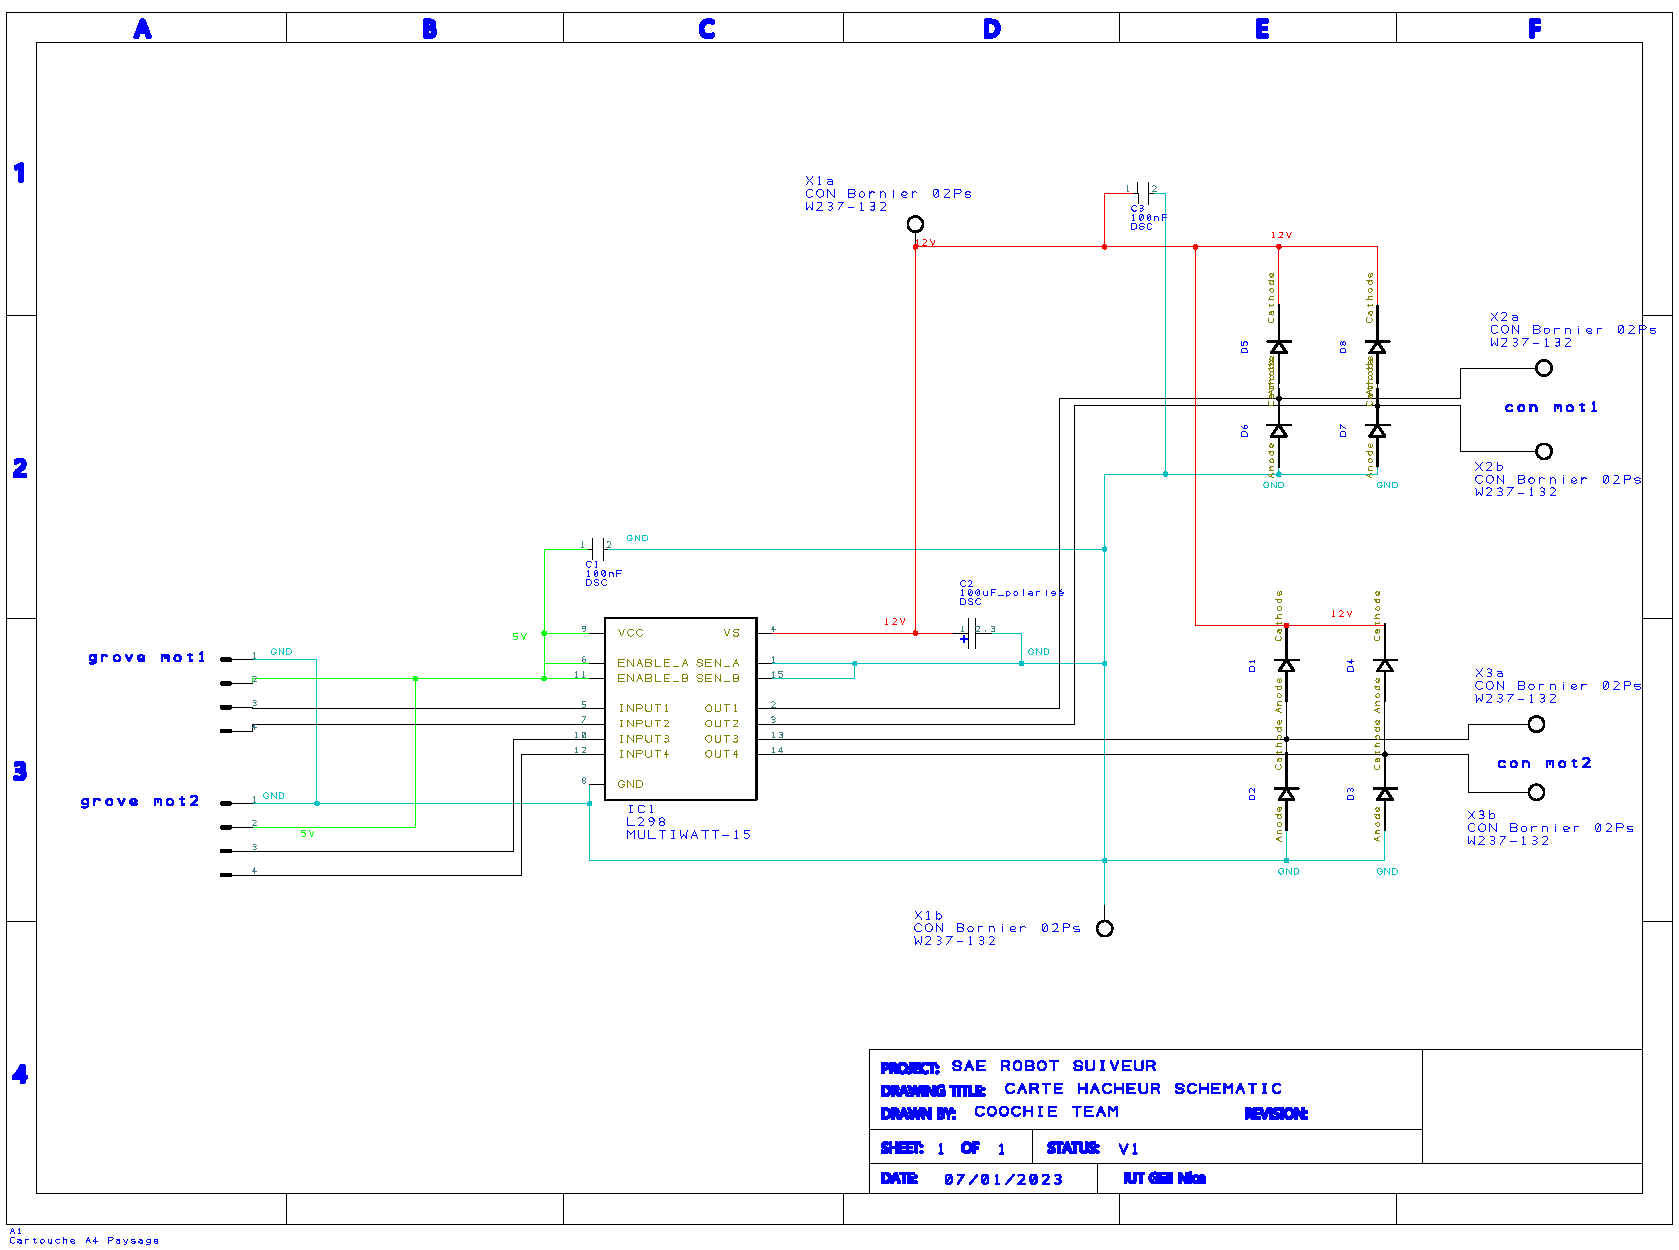
\includepdf[pages=-]{pdf/cartes/hacheur/CarteHacheur - Project.pdf}

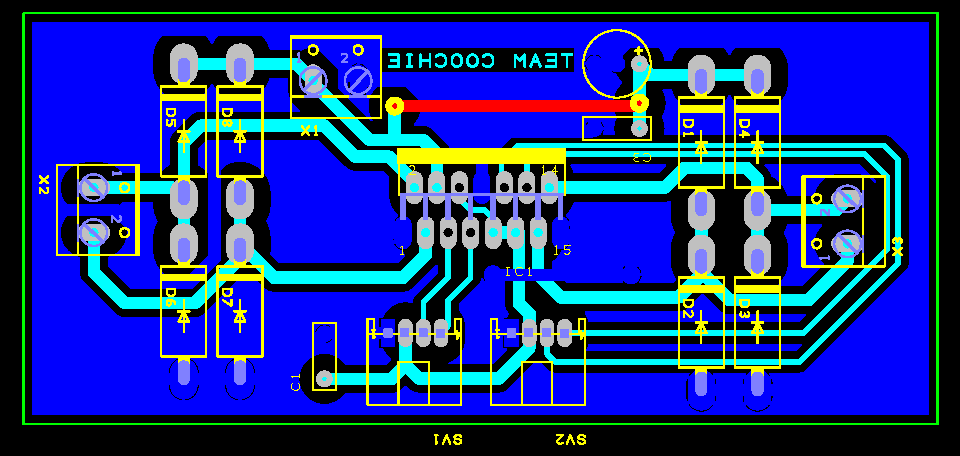
\includepdf[pages=-]{pdf/cartes/hacheur/CarteHacheur - PCB.pdf}

\subsubsection{Carte Commande}

La carte commande est un composant électronique qui permet de contrôler les mouvements du robot. Elle utilise les entrées provenant des capteurs de suivi de ligne pour déterminer où se trouve le robot par rapport à la ligne et donne les instructions nécessaires pour que le robot la suive.

L'utilité de cette carte de commande est d'adapter le système global au format de la MBED. Elle permet de réguler la tension selon en fonction des composants du robot (5V pour la Mbed, 3.3V pour les capteurs etc.). elle permet aussi d'avoir une carte où les entrées et sorties sont centralisées (bornier Grove, octocoupleurs, etc.).
La carte est connectée aux pins GPIO du micro-contrôleur, et rassemble ainsi les informations provenant des capteurs et distribue les ordres du microcontrôleur selon le programme sélectionné.


\begin{figure}[H]
\centering
\begin{minipage}{.5\textwidth}
  \centering
  \centerline{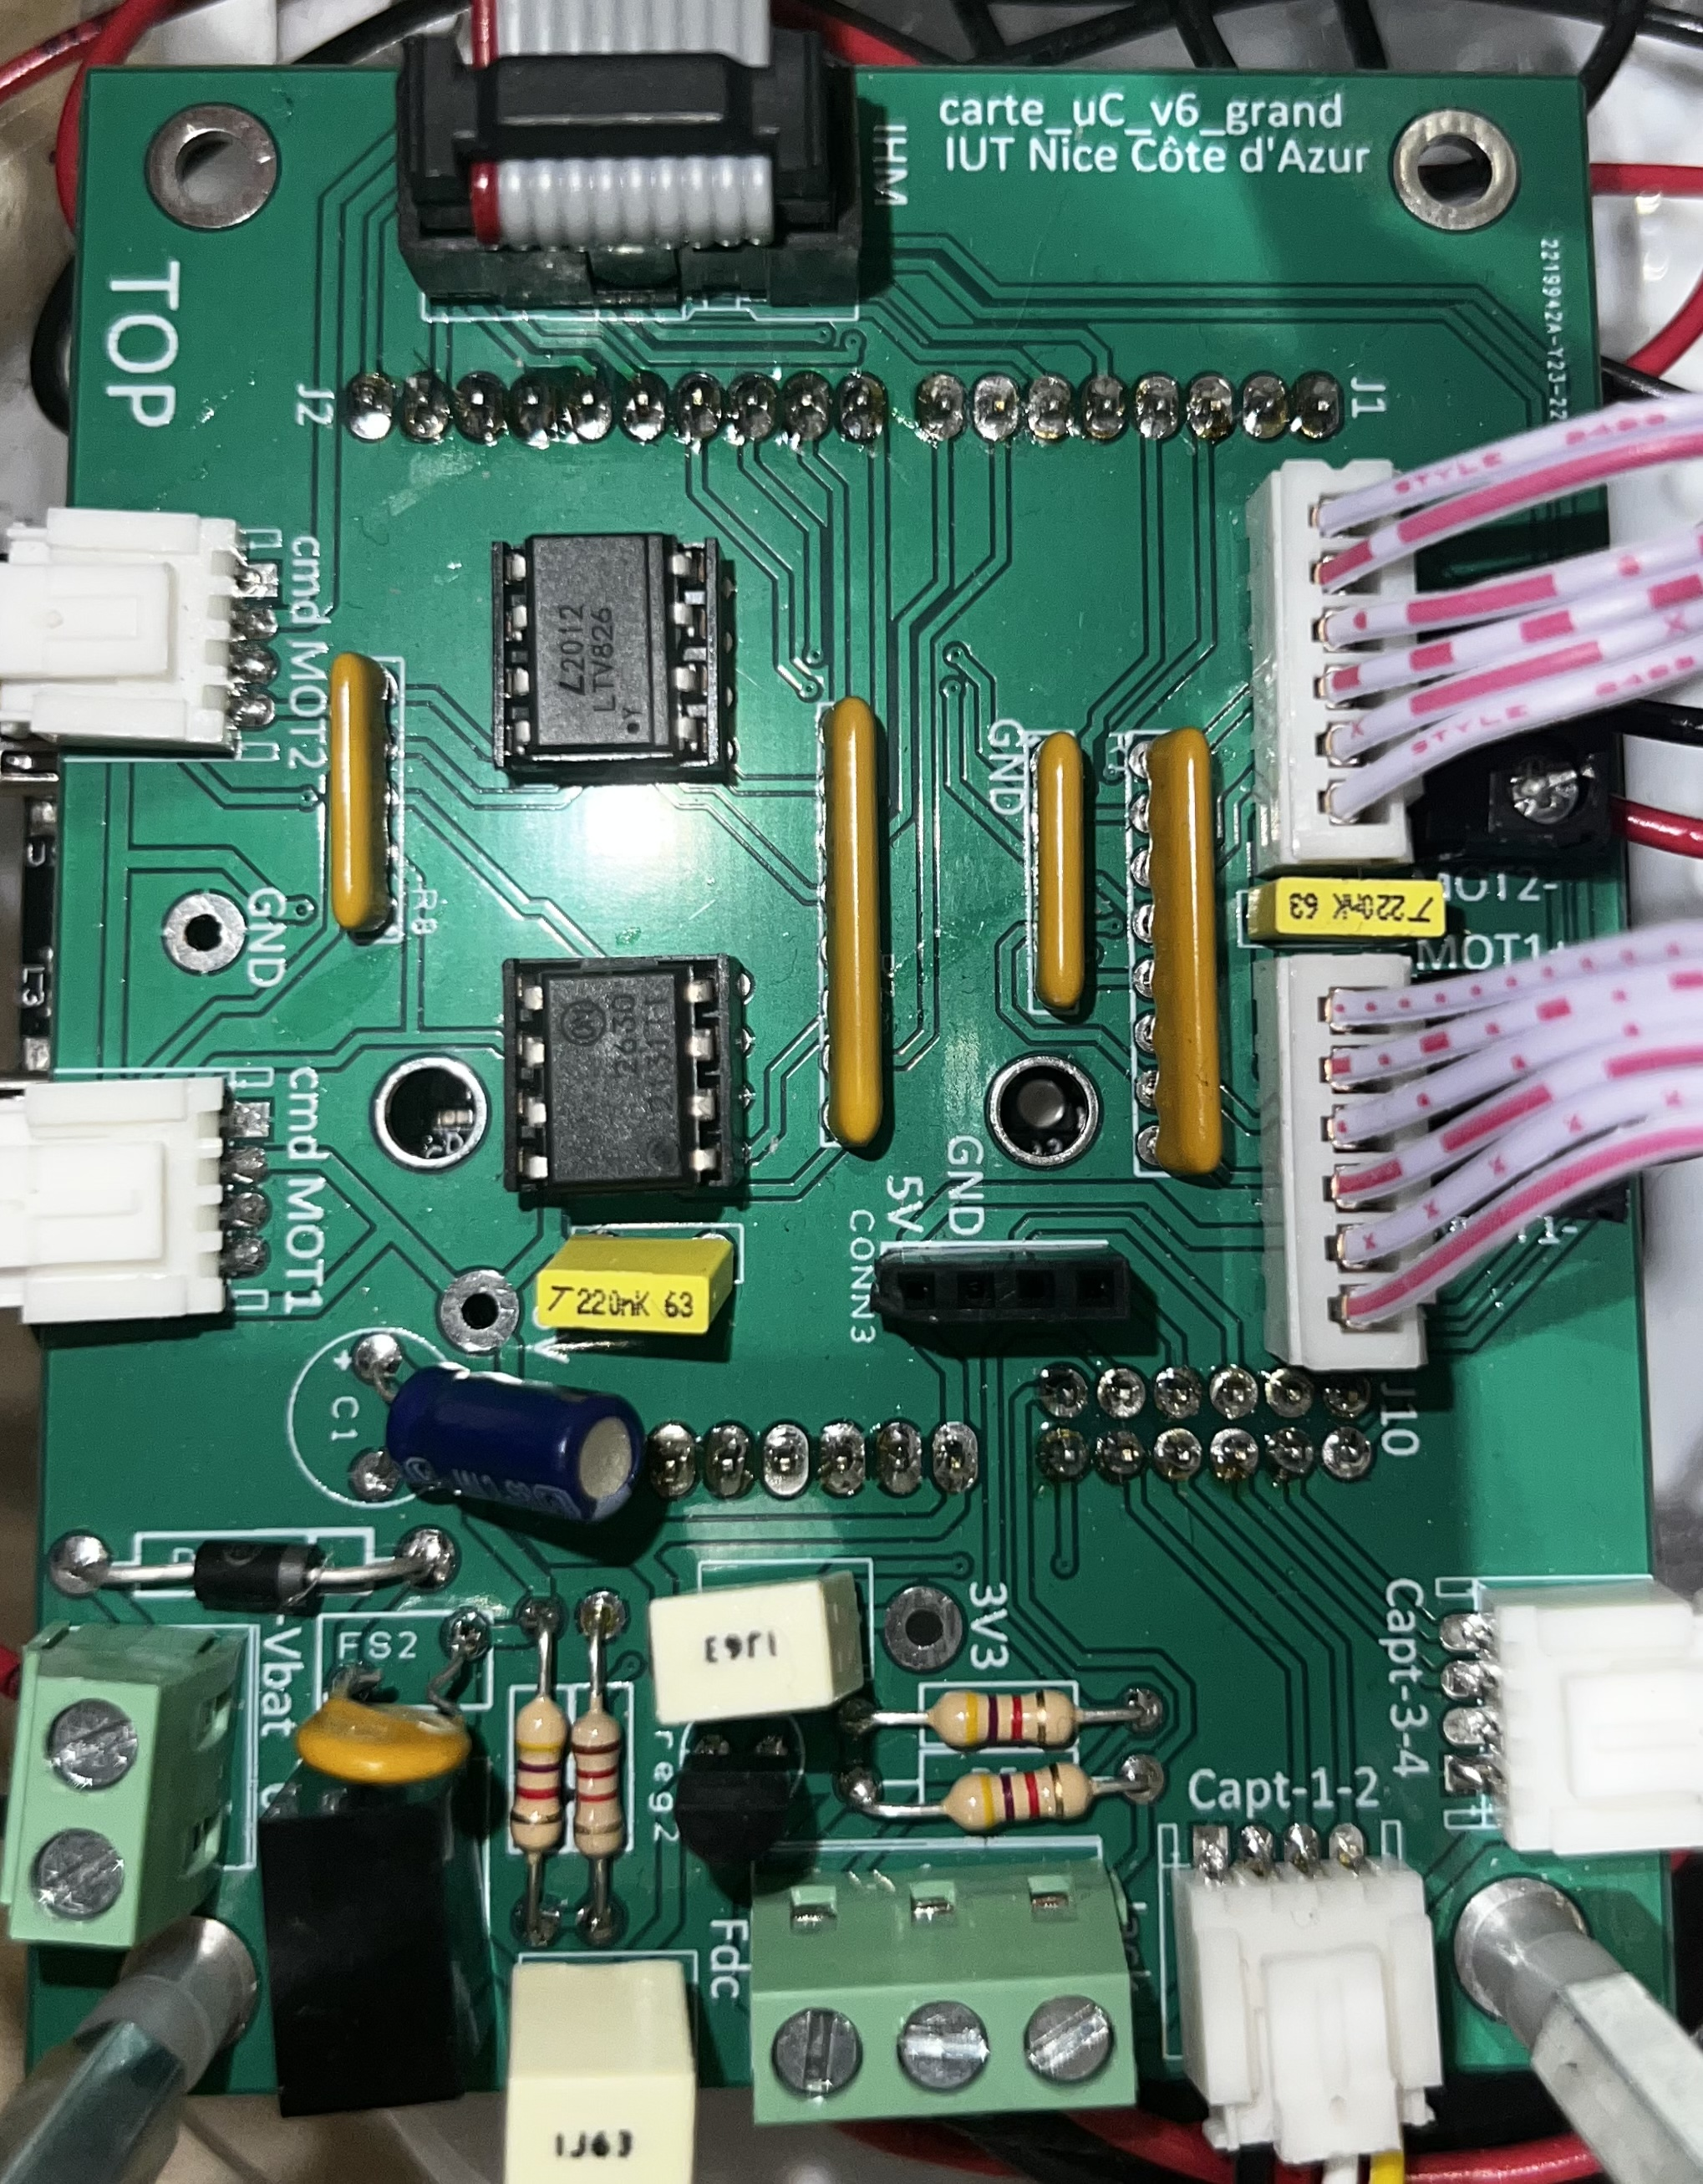
\includegraphics[width=1\linewidth, angle = 90]{img/cartes/commande.jpeg}}
  \captionof{figure}{\emph{Carte Commande}}
  \label{fig:cmd}
\end{minipage}%
\end{figure}

\subsection{Micro-contrôleur}

Le micro-contrôleur est le cerveau de ce projet. En effet, c'est un circuit intégré qui rassemble les éléments essentiels d'un ordinateur : processeur, mémoires (mémoire morte et mémoire vive), unités périphériques et interfaces d'entrées-sorties. 

\vfill
\noindent\makebox[\linewidth]{\rule{.8\paperwidth}{.6pt}}\\[0.2cm]
I.U.T. Nice Côte d'Azur - SAE Robot - 2023 \hfill goofyBot
\noindent\makebox[\linewidth]{\rule{.8\paperwidth}{.6pt}}
\newpage

Dans notre projet, nous utilisons la plateforme de développement FRDM-KL25Z imposée, conçue par l'entreprise Freescale Semiconductor Inc., filiale de NXP. Elle est équipée d'un micro-contrôleur Arm Cortex-M0+ de 48 MHz, 128 KB de mémoire flash (ROM), 16 KB de mémoire vive (RAM). De plus, la MBED est équipée de plusieurs pins GPIO d'entrée/sortie numériques, d'entrée analogiques et de sortie PWM permettant de reçevoir des données et d'interagir avec les moteurs du robot.

En utilisant le logiciel de développement intégré (IDE) Keil Arm Studio Cloud, nous avons pu développer notre code du contrôle du robot en langage C++ (cf. Programmation). À la compilation, l'IDE Keil Studio fournit un fichier \emph{.bin} qui est à placer à la racine du système de fichiers de la MBED. 

\begin{figure}[H]
\centering
\begin{minipage}{.5\textwidth}
  \centering
  \centerline{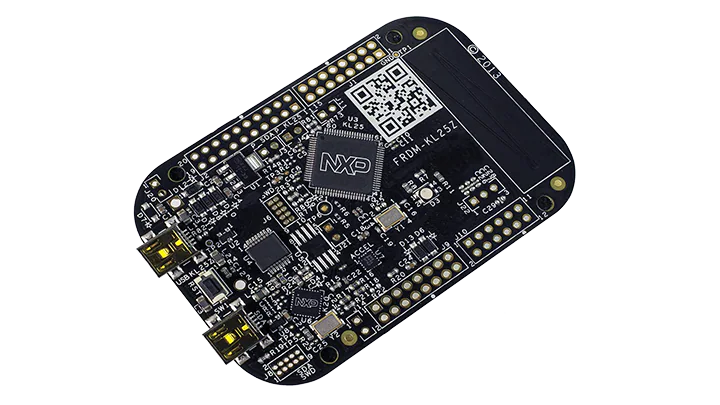
\includegraphics[width=1\linewidth]{img/composants/frdmkl25z.png}}
  \captionof{figure}{\emph{Plateforme de développement FRDM KL25Z}}
  \label{fig:frdmkl25z}
\end{minipage}%
\end{figure}

\vfill
\noindent\makebox[\linewidth]{\rule{.8\paperwidth}{.6pt}}\\[0.2cm]
I.U.T. Nice Côte d'Azur - SAE Robot - 2023 \hfill goofyBot
\noindent\makebox[\linewidth]{\rule{.8\paperwidth}{.6pt}}
\newpage
\section{Programmation}

\subsection{Programmation orientée objet (POO)}

Nous avons fait le choix d'utiliser une fonctionnalité très utile du langage C++, la programmation orientée objet. La programmation orientée objet (POO) est un moyen de concevoir et de construire des programmes informatiques en utilisant des \emph{objets}.

Chaque objet a des caractéristiques, telles que l'apparence ou les fonctionnalités, qui sont décrites dans un plan appelé \emph{classe}. La classe définit comment l'objet doit se comporter et quoi faire lorsqu'on lui envoie des messages ou des instructions.

L'objectif de la POO est de modéliser le monde réel en utilisant des objets qui représentent des entités réelles, telles que des personnes, des voitures ou des robots. Les objets peuvent interagir les uns avec les autres en envoyant des messages et en appelant des \emph{méthodes}.

La POO est largement utilisée dans la programmation moderne et est prise en charge par de nombreux langages de programmation, tels que Java, Python, C++ et bien d'autres. En utilisant la POO, les développeurs peuvent créer des programmes plus robustes, plus flexibles et plus faciles à maintenir.

\noindent Dans le cas de notre projet, nous avons un objet \emph{Robot}, nommé \textbf{\textit{goofyBot}} tout au long du projet, initialisé avec des valeurs du constructeur :

\begin{lstlisting}[language={C++}, caption={Fichier robot.hpp contenant la classe Robot}, label={robot.hpp}]
#ifndef ROBOT_HPP
#define ROBOT_HPP

#include <mbed.h>

class Robot {

public:
    Robot();

    DigitalOut IHM_Led1;
    DigitalOut IHM_Led2;
    DigitalOut IHM_Led3;
    DigitalOut IHM_Led4;

    DigitalIn IHM_Btn1;
    DigitalIn IHM_Btn2;
    DigitalIn IHM_Btn3;
    DigitalIn IHM_Btn4;

    DigitalIn jack;
    DigitalIn finCourse;
    AnalogIn mesureBatterie;
    AnalogIn captLigneDroiteInt;
    AnalogIn captLigneDroiteExt;
    AnalogIn captLigneGaucheInt;
    AnalogIn captLigneGaucheExt;

    PwmOut moteurDroit;
    PwmOut moteurGauche;
    DigitalOut moteurDroitSens;
    DigitalOut moteurGaucheSens;

    int jackVal;
    int fcVal;
    double mbVal;
    double dIntVal;
    double dExtVal;
    double gIntVal;
    double gExtVal;

    /** Fonction de debug du robot
     *  Affiche les valeurs des capteurs sur le port série.
     * 
     *  @note Teste les capteurs de ligne, de fin de course, de batterie et le jack et 
     *  démarre en même temps le mode débug de l'IHM.
     * 
     *  @warning Le robot doit être connecté à un ordinateur pour afficher les valeurs sur le port série.
     */
    void debugMode();

    /** Déplace le robot en fonction des PWMs des moteurs gauche et droit et des sens des moteurs
     *
     *  @param pwmGauche Valeur du PWM du moteur gauche entre -100 et 100 (reverse et forward)
     *  @param pwmDroit Valeur du PWM du moteur droit entre -100 et 100 (reverse et forward)
     */
    void move(float pwmGauche, float pwmDroit);
};

#endif

\end{lstlisting}

\begin{lstlisting}[language={C++}, caption={Constructeur de la classe Robot}, label={robot.cpp}]
// Constructeur
Robot::Robot() :
    // Assignation des pins
    jack(PTE20),
    finCourse(PTE21),
    mesureBatterie(A0),
    captLigneDroiteInt(A1),
    captLigneDroiteExt(A2),
    captLigneGaucheInt(A4),
    captLigneGaucheExt(A3),

    IHM_Led1(D15),
    IHM_Led2(D14),
    IHM_Led3(D13),
    IHM_Led4(D12),
    IHM_Btn1(D4),
    IHM_Btn2(D5),
    IHM_Btn3(A5),
    IHM_Btn4(PTE30),

    moteurDroit(D6),
    moteurGauche(D8),
    moteurDroitSens(D7),
    moteurGaucheSens(D9)
{ 
    // Initialisation des moteurs
    moteurDroitSens = 1;
    moteurGaucheSens = 1;
}

\end{lstlisting}

\subsection{Contrôler le robot}

Afin de faire fonctionner les moteurs grâce à la carte hacheur, nous avons une fonction appelée \emph{move} qui permet de contrôler le mouvement des moteurs du robot. Elle fait partie de la classe "Robot" et est donc accessible à tous les objets de ce type.

La fonction prend en entrée deux variables "pwmGauche" et "pwmDroit", qui représentent les niveaux de puissance pour les moteurs gauche et droit respectivement. La valeur de ces variables peut varier de -100 à 100. Si la valeur est positive, le moteur tourne dans un sens (sens avant), et si la valeur est négative, il tourne dans l'autre sens (sens arrière). Si la valeur est nulle, le moteur est arrêté.

La fonction définit tout d'abord la période pour les moteurs gauche et droit. Ensuite, le code effectue un certain nombre de calculs pour déterminer le sens de rotation du moteur et le niveau de puissance pour chaque moteur en fonction de la valeur d'entrée.

En somme, cette fonction permet de contrôler les moteurs du robot en fonction des entrées fournies, ce qui peut être utilisé pour contrôler le mouvement du robot dans différentes directions.

\begin{lstlisting}[language={C++}, caption={Fonction move()}, label={robot.cpp}]
void Robot::move(float pwmGauche, float pwmDroit) {
    // On définit la période des moteurs
    moteurDroit.period(T);
    moteurGauche.period(T);

    if(pwmGauche >= -100.0 && pwmGauche < 0) {
        moteurGaucheSens = 0; // Sens arrière
        pwmGauche = pwmGauche * -1.0;
        pwmGauche = pwmGauche / 100.0; // On divise par 100 pour avoir un pwm entre 0 et 1
    } else if (pwmGauche <= 100 && pwmGauche > 0) {
        moteurGaucheSens = 1; // Sens avant
        pwmGauche -= 100.0;
        pwmGauche = pwmGauche * -1.0;
        pwmGauche = pwmGauche / 100.0;
    } else if (pwmGauche == 0) {
        moteurGaucheSens = 1;
        pwmGauche = 1; // Stop
    }

    if(pwmDroit >= -100.0 && pwmDroit < 0) {
        moteurDroitSens = 0; // Sens arrière
        pwmDroit = pwmDroit * -1.0; // On inverse le signe du pwm
        pwmDroit = pwmDroit / 100.0; // On divise par 100 pour avoir un pwm entre 0 et 1
        //printf("%f", pwmDroit);
    } else if (pwmDroit <= 100 && pwmDroit > 0) {
        moteurDroitSens = 1; // Sens avant
        pwmDroit = pwmDroit - 100.0; 
        pwmDroit = pwmDroit * -1.0;
        pwmDroit = pwmDroit / 100.0; // On divise par 100 pour avoir un pwm entre 0 et 1
    } else if (pwmDroit == 0) {
        moteurDroitSens = 1;
        pwmDroit = 1; // Stop
    }

    // On applique le pwm aux moteurs
    moteurDroit.pulsewidth(T * pwmDroit);
    moteurGauche.pulsewidth(T * pwmGauche);
}

\end{lstlisting}

\subsection{Programmes}

La partie programmation du robot est séparée en trois fonctions principales du robot : deux fonctions permettant l'homologation du robot (Confettis et Carré) et la fonction suivi de ligne.

\subsubsection{Les confettis}

\begin{figure}[H]
\centering
\begin{minipage}{.5\textwidth}
  \centering
  \centerline{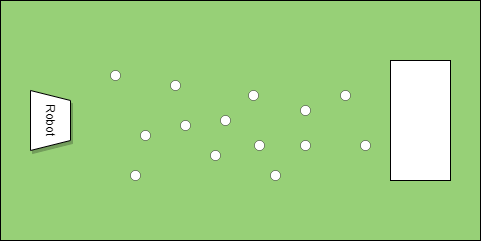
\includegraphics[width=1\linewidth]{img/parcours/confettie.png}}
  \captionof{figure}{\emph{Le robot doit passer par un chemin parsemé de confettis.}}
  \label{fig:confettis}
\end{minipage}%
\end{figure}

\vfill
\noindent\makebox[\linewidth]{\rule{.8\paperwidth}{.6pt}}\\[0.2cm]
I.U.T. Nice Côte d'Azur - SAE Robot - 2023 \hfill goofyBot
\noindent\makebox[\linewidth]{\rule{.8\paperwidth}{.6pt}}
\newpage

Cette fonction, nommée "confettis", utilise la bibliothèque "mbed" et la classe "Robot" définie dans "robot.hpp". Elle implémente un programme pour faire bouger un robot suiveur de ligne.

La fonction utilise une boucle infinie (while (1)) pour continuer à faire bouger le robot. A chaque tour de boucle, les entrées du robot (état de la valeur des capteurs de ligne) sont actualisées.

Ensuite, deux \emph{switchs} sont utilisés pour déterminer l'état du robot en fonction des entrées. Le premier switch détermine l'état suivant du robot en fonction de ses entrées actuelles, et le second switch détermine les actions à prendre pour chaque état. (cf. Machine à états)

\begin{figure}[H]
\centering
\begin{minipage}{.5\textwidth}
  \centering
  \centerline{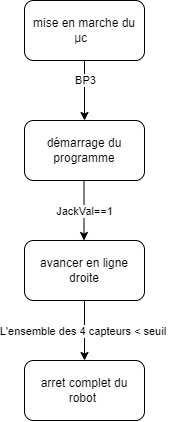
\includegraphics[width=0.5\linewidth]{img/mae/confettis.png}}
  \captionof{figure}{\emph{Machine à états : Confettis}}
  \label{fig:maeconfettis}
\end{minipage}%
\end{figure}

Par exemple, si le Jack est retiré (\emph{goofyBot.jackVal == 1}), l'état du robot passe à 2 et le robot bouge en avant (goofyBot.move(50,50)). Si les quatre capteurs de ligne détectent la ligne blanche (\emph{goofyBot.dIntVal <= 0.5 \&\& goofyBot.dExtVal <= 0.5 \&\& goofyBot.gIntVal <= 0.5 \&\& goofyBot.gExtVal <= 0.5}), alors l'état du robot passe à 4 et le robot attend pendant 25 000 microsecondes puis s'arrête (\emph{goofyBot.move(0,0)}).

\begin{lstlisting}[language={C++}, caption={Fonction confettis()}, label={confettis.cpp}]
void confettis(Robot& goofyBot) {
    int etat = 1;
    
    while (1) {
        goofyBot.jackVal = goofyBot.jack.read();
        goofyBot.dIntVal = goofyBot.captLigneDroiteInt.read() * 3.3;
        goofyBot.dExtVal = goofyBot.captLigneDroiteExt.read() * 3.3;
        goofyBot.gIntVal = goofyBot.captLigneGaucheInt.read() * 3.3;
        goofyBot.gExtVal = goofyBot.captLigneGaucheExt.read() * 3.3;

        switch(etat) {
            case 1:
                if (goofyBot.jackVal == 1) {
                    etat = 2;
                }
                break;
            
            case 2:
                if(goofyBot.dIntVal <= 0.5 && goofyBot.dExtVal <= 0.5 && goofyBot.gIntVal <= 0.5 && goofyBot.gExtVal <= 0.5) {
                    etat = 4;
                }
                break;
        }

        switch(etat) {
            case 2 :
                goofyBot.move(50,50);
                break;

            case 4 :
                wait_us(25000);
                goofyBot.move(0,0);
                break;
        }
    }
}
\end{lstlisting}

\subsubsection{Le carré}

\begin{figure}[H]
\centering
\begin{minipage}{.5\textwidth}
  \centering
  \centerline{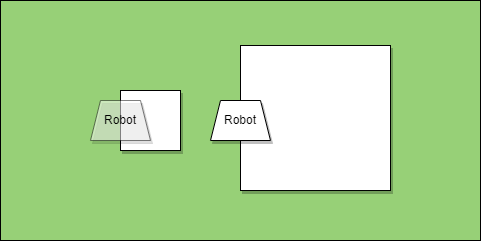
\includegraphics[width=1\linewidth]{img/parcours/carre.png}}
  \captionof{figure}{\emph{Le robot doit réaliser un carré.}}
  \label{fig:carre}
\end{minipage}%
\end{figure}

Ce code définit une fonction \emph{carre} qui fait que le robot exécute une forme carrée. La longueur du carré est déterminée par l'utilisateur via la fonction \emph{ihmSel()}. Le code utilise la méthode \emph{move()} de l'objet Robot pour contrôler le mouvement du robot. 

\vfill
\noindent\makebox[\linewidth]{\rule{.8\paperwidth}{.6pt}}\\[0.2cm]
I.U.T. Nice Côte d'Azur - SAE Robot - 2023 \hfill goofyBot
\noindent\makebox[\linewidth]{\rule{.8\paperwidth}{.6pt}}
\newpage

La fonction carré fait d'abord avancer le robot à vitesse constante sur une distance définie, puis fait tourner le robot en augmentant et en diminuant la vitesse des deux roues à des vitesses différentes. Le processus est répété 4 fois pour former une forme carrée.

\begin{figure}[H]
\centering
\begin{minipage}{.5\textwidth}
  \centering
  \centerline{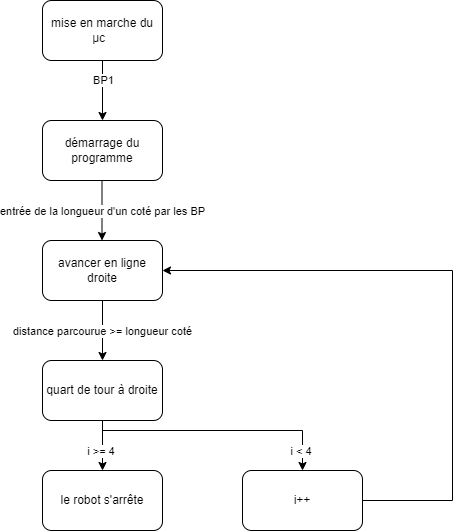
\includegraphics[width=1\linewidth]{img/mae/carre.png}}
  \captionof{figure}{\emph{Machine à états : Carré}}
  \label{fig:maecarre}
\end{minipage}%
\end{figure}

\begin{lstlisting}[language={C++}, caption={Fonction carre()}, label={carre.cpp}]
void carre(Robot& goofyBot) {
    int longueur = ihmSel(goofyBot);

    for(int i = 0; i < 4; i++) {
        goofyBot.move(45,45);
        wait_us ((longueur / 45.5) * 1000000) ;
        goofyBot.move(0,0);
        wait_us(500000);
        // augmentation et diminution progressive de la vitesse
        for(float speed = 25; speed < 90; speed += 5) {
            goofyBot.move(speed, -70);
            wait_us(14000);
        }
        for(float speed = 100; speed > 90; speed -= 5) {
            goofyBot.move(speed, -70);
            wait_us(14000);
        }
    }

    goofyBot.move(0,0);
}
\end{lstlisting}

\vfill
\noindent\makebox[\linewidth]{\rule{.8\paperwidth}{.6pt}}\\[0.2cm]
I.U.T. Nice Côte d'Azur - SAE Robot - 2023 \hfill goofyBot
\noindent\makebox[\linewidth]{\rule{.8\paperwidth}{.6pt}}
\newpage

Comme décrit ci-dessus, le côté du carré réalisé devra être compris entre 60cm et 200cm (2m). Pour cela, nous avons implémenté la fonction \emph{ihmSel()}. Celle-ci utilise l'intégralité de la carte IHM pour fonctionner. En effet, nous avons deux boutons de choix de taille (+10cm et +100cm) et deux boutons de validation (Reset et Valider).

\begin{lstlisting}[language={C++}, caption={Fonction ihmSel()}, label={ihm.cpp}]
int ihmSel(Robot& goofyBot) {
    // Taille en CM du carré (entre 60 et 200)
    int res = 0;
    while(goofyBot.IHM_Btn4.read() == 0) {
        goofyBot.IHM_Led2.write(0);
        if (goofyBot.IHM_Btn1.read() == 1) {
            // Ajout dizaines
            res += 10;
            wait_us(1000000);
        }
        else if (goofyBot.IHM_Btn2.read() == 1) {
            // Ajout centaines
            res += 100;
            wait_us(1000000);

        }
        else if (goofyBot.IHM_Btn3.read() == 1) {
            // Reset
            res = 0;
            wait_us(1000000);
        }
        
    }
    if(res > 200 || res < 60) {
        res = 0;
        for(int i = 0; i < 5; i++) {
            goofyBot.IHM_Led4.write(0);
            wait_us(100000);
            goofyBot.IHM_Led4.write(1);
            wait_us(100000);
        }
    }

    goofyBot.IHM_Led2.write(1);

    for(int i = 0; i < 5; i++) {
        goofyBot.IHM_Led1.write(0);
        wait_us(500000);
        goofyBot.IHM_Led1.write(1);
        wait_us(500000);
    }

    goofyBot.IHM_Led2.write(0);

    return res;
}
\end{lstlisting}

\vfill
\noindent\makebox[\linewidth]{\rule{.8\paperwidth}{.6pt}}\\[0.2cm]
I.U.T. Nice Côte d'Azur - SAE Robot - 2023 \hfill goofyBot
\noindent\makebox[\linewidth]{\rule{.8\paperwidth}{.6pt}}
\newpage

\subsubsection{Le suivi de ligne}

Et enfin, la dernière fonction et la plus importante, le suivi de ligne.

\begin{figure}[H]
\centering
\begin{minipage}{.5\textwidth}
  \centering
  \centerline{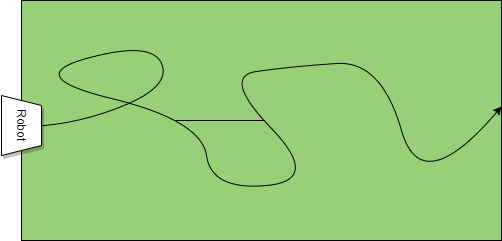
\includegraphics[width=1\linewidth]{img/parcours/suivideligne.png}}
  \captionof{figure}{\emph{Le robot doit suivre la ligne.}}
  \label{fig:suiviligne}
\end{minipage}%
\end{figure}

Afin de pouvoir allier vitesse et précision, nous avons décidé d'intégrer l'algorithme PID (\emph{Proportional-Integral-Derivative}), qui est un algorithme de contrôle utilisé pour maintenir une quantité mesurée, telle que la position, la vitesse ou la température, à une valeur souhaitée. Il est souvent utilisé  en automatisme et notamment dans la robotique pour contrôler les moteurs d'un robot ou d'un drone afin de maintenir une position ou une vitesse cible.   

L'algorithme PID utilise trois termes pour calculer le signal de commande pour les moteurs :

Proportionnel (P) : Le terme proportionnel est basé sur l'erreur actuelle entre la valeur mesurée et la valeur cible. Plus l'erreur est grande, plus le signal de commande sera fort.

Intégral (I) : Le terme intégral prend en compte l'accumulation de l'erreur au fil du temps. Cela peut aider à éliminer les erreurs à long terme et à améliorer la stabilité du système. (non utilisé ici)

Dérivative (D) : Le terme dérivatif est basé sur la vitesse de changement de l'erreur. Il peut aider à améliorer la réactivité du système et à éviter les oscillations.Plus il est élevé plus on tendra rapidement a la valeur de stabilité.

Les trois termes sont combinés pour produire le signal de commande pour les moteurs. Les constantes \textit{Kp}, \textit{Ki} et \textit{Kd} sont les gains PID qui peuvent être ajustés pour optimiser les performances du système de contrôle. Ils entrent aussi en équation avec la vitesse qu'il faut aussi régler avec précision pour obtenir un suivi de ligne optimal alliant fiabilité et rapidité.

\vfill
\noindent\makebox[\linewidth]{\rule{.8\paperwidth}{.6pt}}\\[0.2cm]
I.U.T. Nice Côte d'Azur - SAE Robot - 2023 \hfill goofyBot
\noindent\makebox[\linewidth]{\rule{.8\paperwidth}{.6pt}}
\newpage

\begin{figure}[H]
\centering
\begin{minipage}{.5\textwidth}
  \centering
  \centerline{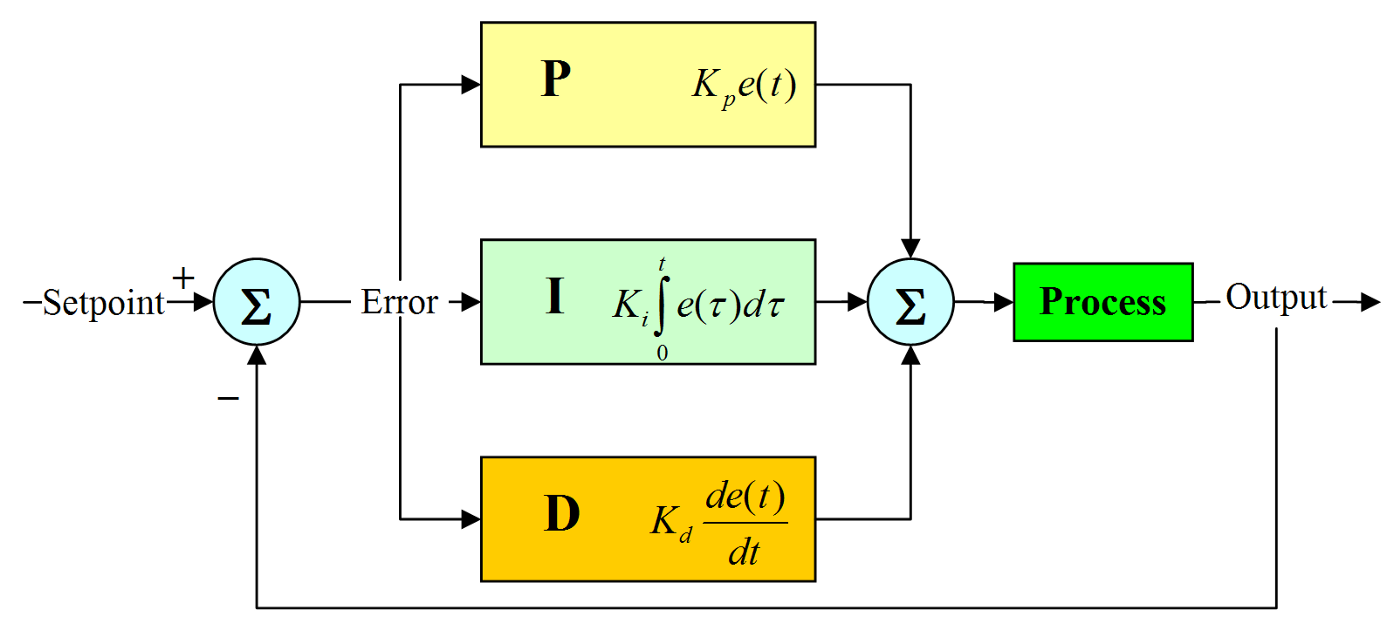
\includegraphics[width=1.2\linewidth]{img/pid.png}}
  \captionof{figure}{\emph{Schéma de l'algorithme PID.}}
  \label{fig:PID}
\end{minipage}%
\end{figure}

\begin{center}
    $u(t) = Kp * e(t) + Ki * \int_{0}^{t} e(\tau) \,d\tau + Kd \frac{de}{dt}(t)$
    
    Formule de l'algorithme PID prenant en compte les coefficients \emph{Kp, Kd et Ki}
\end{center}

\begin{lstlisting}[language={C++}, caption={Fonction suivi()}, label={suivi.cpp}]
#define SPEED 75
#define KP 45
#define KD 55

void suivi(Robot& goofyBot) {

    int etat = 0;
    float error = 0;
    float last_error = 0;
    float integral = 0;
    float derivative = 0;
    float PID_value, e, errorD, errorG;

    while(true) {
        goofyBot.jackVal = goofyBot.jack.read();
        goofyBot.fcVal = goofyBot.finCourse.read();
        goofyBot.dIntVal = goofyBot.captLigneDroiteInt.read();
        goofyBot.dExtVal = goofyBot.captLigneDroiteExt.read()*3.3;
        goofyBot.gIntVal = goofyBot.captLigneGaucheInt.read();
        goofyBot.gExtVal = goofyBot.captLigneGaucheExt.read()*3.3;
    
        e = ((goofyBot.gIntVal*3.3) - (goofyBot.dIntVal*3.3));

        error = (goofyBot.gIntVal - goofyBot.dIntVal);

        errorD = (goofyBot.dExtVal - goofyBot.gIntVal);
        errorG = (goofyBot.gExtVal - goofyBot.dIntVal);

        derivative = error - last_error;
        last_error = error;
        PID_value = (KP*error) + (KD*derivative);
        
        if(goofyBot.fcVal == 0) {
            etat = 69;
        }

        switch(etat) {
            case 0:
                if(goofyBot.jackVal == 1) {
                    etat = 1; //suivi
                } 
                break;
            
            case 1:
                if(e >= -0.05 || e <= 0.05) {
                    etat = 2;
                }
                break;

            case 2:
                if(goofyBot.dExtVal < 1.5 || goofyBot.gExtVal < 1.5) { //case extreme
                    etat = 3;
                }
                if (e >= 0.10 && e <= -0.10) {
                    etat = 1;
                }
                break;

            case 3: 
                if (e <= 0.02 && e >= -0.02) {
                    etat = 1;
                }
                if(e <= -0.10 && e >= 0.10) {
                    etat = 2;
                }
                break;
        }

        switch(etat) {
            case 0:
                if(e <= 0.03 && e >= -0.03) {
                    goofyBot.IHM_Led3.write(1);    
                } else {
                    goofyBot.IHM_Led3.write(0);
                }
                goofyBot.move(0,0);
                break;

            case 1:
                goofyBot.move(50,50);
                break;

            case 2:
                goofyBot.move(SPEED + PID_value, SPEED - PID_value);
                break;

            case 3:
                if(goofyBot.dExtVal < 0.7 || e >= 0.85) {
                    PID_value = (KP*errorD) + (KD*derivative);
                    goofyBot.move(SPEED + 10 + PID_value,0);
                }
                if(goofyBot.gExtVal < 0.7 || e >= 0.85) {
                    PID_value = (KP*errorG) + (KD*derivative);
                    goofyBot.move(0, SPEED + 10 + PID_value);
                }
                break;

            case 69: 
                goofyBot.move(0,0);
                break;
            }
        wait_us(5000);
    }
}
\end{lstlisting}

\vfill
\noindent\makebox[\linewidth]{\rule{.8\paperwidth}{.6pt}}\\[0.2cm]
I.U.T. Nice Côte d'Azur - SAE Robot - 2023 \hfill goofyBot
\noindent\makebox[\linewidth]{\rule{.8\paperwidth}{.6pt}}
\newpage

Ce code utilise l'algorithme PID pour suivre une ligne avec un robot. Il implémente une boucle de contrôle qui utilise des entrées de capteurs pour déterminer l'état actuel du robot et déterminer la prochaine action à effectuer. Les différents états incluent l'arrêt, le suivi de ligne droite et le virage à gauche ou à droite selon la position de la ligne.

Le code définit les constantes KP et KD pour le contrôleur PID. KP représente la proportionnalité, KD représente la dérivée, qui permet d'ajuster la réponse en fonction de la vitesse de changement de l'erreur. L'erreur est calculée en comparant les entrées des capteurs de ligne gauche et droite.

L'état est géré en utilisant un \emph{switch case} qui vérifie la valeur de l'état à chaque itération de la boucle de contrôle. En fonction de l'état, des actions différentes sont prises pour faire avancer ou tourner le robot. Par exemple, lorsque le robot se trouve dans l'état 1, il avance droit. Lorsqu'il se trouve dans l'état 3, il tourne selon la position de la ligne.

\begin{figure}[H]
\centering
\begin{minipage}{.5\textwidth}
  \centering
  \centerline{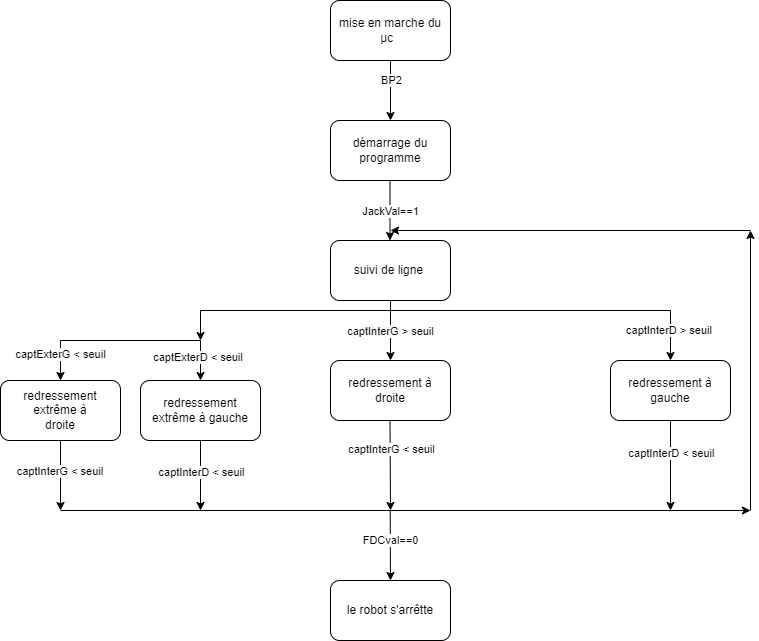
\includegraphics[width=1.2\linewidth]{img/mae/suivi ligne.png}}
  \captionof{figure}{\emph{Machine à états : suiveur de ligne.}}
  \label{fig:maesuiviligne}
\end{minipage}%
\end{figure}

Enfin, la fonction \emph{wait\_us(5000)} permet de définir un délai de 5 millisecondes entre chaque itération de la boucle de contrôle, ce qui permet d'éviter les erreurs de lecture des capteurs et de contrôler la vitesse du robot.

\subsubsection{Les options}
Dans ce projet nous avons eu la possibilité d’intégrer à nos codes des options nous rapportant des bonus, les 3 principales sont : 

\vfill
\noindent\makebox[\linewidth]{\rule{.8\paperwidth}{.6pt}}\\[0.2cm]
I.U.T. Nice Côte d'Azur - SAE Robot - 2023 \hfill goofyBot
\noindent\makebox[\linewidth]{\rule{.8\paperwidth}{.6pt}}
\newpage

\begin{itemize}
    \item Le raccourci : C’est une extension du programme suiveur de ligne, ce programme consiste en l’action de prendre un raccourci et donc automatiquement gagner du temps de parcours. Pour voir le raccourci, un bout de piste (ligne blanche) est placé 30cm en amont de la bifurcation, à gauche de la piste obligatoirement. Ce marqueur nous permet d’ordonner au robot de prendre le raccourci, et donc de tourner à gauche de 90°. Pour programmer le raccourci, en théorie d’abord,nous avons pensé créer une variable erreur gauche qui est égale a la tension du capteur extérieur gauche moins la tension du capteur intérieur droit. Il y en a une deuxième qui est la variable erreur droite qui prend pour valeur la tension du capteur extérieur droit moins la tension du capteur intérieur gauche. Ensuite, ces deux variables sont comparées et si le résultat de cette comparaison est supérieure à un seuil c’est qu' un marqueur a été repéré et donc qu'il va falloir tourner pour la piste de raccourci.

    \item Le stop-figure : Le stop figure est bonus de temps qui sera soustrait au temps final de suivi de ligne. Il consiste en l’arrêt du robot pendant le suivi de ligne ou après et la réalisation d’un tout du robot sur lui-même à 360°. Si il est réalisé pendant c’est un bonus de 10 secondes, et si il est après l’arrêt du robot, au fin de course, c’est 3 secondes de bonus. Pour coder celui-ci, théoriquement nous avons pensé utiliser un timer que l’on déclare avec la bibliothèque “time.h”, puis une variable tempsDebut et une autre tempsActuel. tempsDebut est affecté de la valeur de temps au début du programme et tempsActuel est  égale a tempsDebut et est en plus incrémentée en continu. Puis une simple comparaison avec une constante définie au début qui est en secondes pour savoir au bout de combien de temps on fait le stop Figure, nous envoie dans un état qui envoie aux bornes du moteur la même tension en sens inverse pendant le temps qu’il faut pour faire un tour. Une fois le tour fini, l’état redevient à celui du suivi.

    \item La priorité à droite : Celle- ci est moins importante, car n'apporte pas de bonus et nous ne l’avons pas faite, faute de temps. Cette option se résume à l'intégration d’un capteur supplémentaire sur le haut du robot tourné vers la droite et qui doit identifier qu’un robot arrive à droite et le laisse passer pendant le suivi de ligne.
\end{itemize}

\vfill
\noindent\makebox[\linewidth]{\rule{.8\paperwidth}{.6pt}}\\[0.2cm]
I.U.T. Nice Côte d'Azur - SAE Robot - 2023 \hfill goofyBot
\noindent\makebox[\linewidth]{\rule{.8\paperwidth}{.6pt}}
\newpage
\section{Travail en groupe}
Ce projet nous a permis de goûter à la réalisation d'un travail sur un sujet poussé et nouveau, et ce sur une longue durée et en groupe. Cela nous a donc poussé à parfaire notre adaptation, que ce soit au niveau de notre emploi du temps, ou même par rapport aux autres membres du groupe. Les prises de décisions, l'organisation, et les méthodes pour mettre à bien notre projet étaient à décider en équipe, ce qui nous a aussi permi de nouer des liens entre nous. La grande majorité du groupe étant jeune, et fraîchement sortie du lycée, les concepts de managment d'équipe et d'abnégation pour réaliser un travail étaient nouveaux, et très enrichissants pour des étudiants comme nous.

Aussi, nous avons evidemment dû surmonter de multiples difficultés, au fil de la réalisation du robot.

La soudure étant une pratique totalement nouvelle pour tous, nous avons dû prendre un certain temps afin de la maîtriser du moins assez correctement pour la pratiquer directement sur nos propres cartes. Elle a donc été source de plusieurs soucis au long du projet. Certains points de soudures ont parfois été mal réalisés, des composants placés à l'envers ont créé des court circuits que nous avons  dû nous même identifier, etc.

Le suivi de projet, a été tenu sur GitHub, afin de pouvoir centraliser les documents du groupe.

\begin{figure}[H]
\centering
\begin{minipage}{.5\textwidth}
  \centering
\href{}{}  \centerline{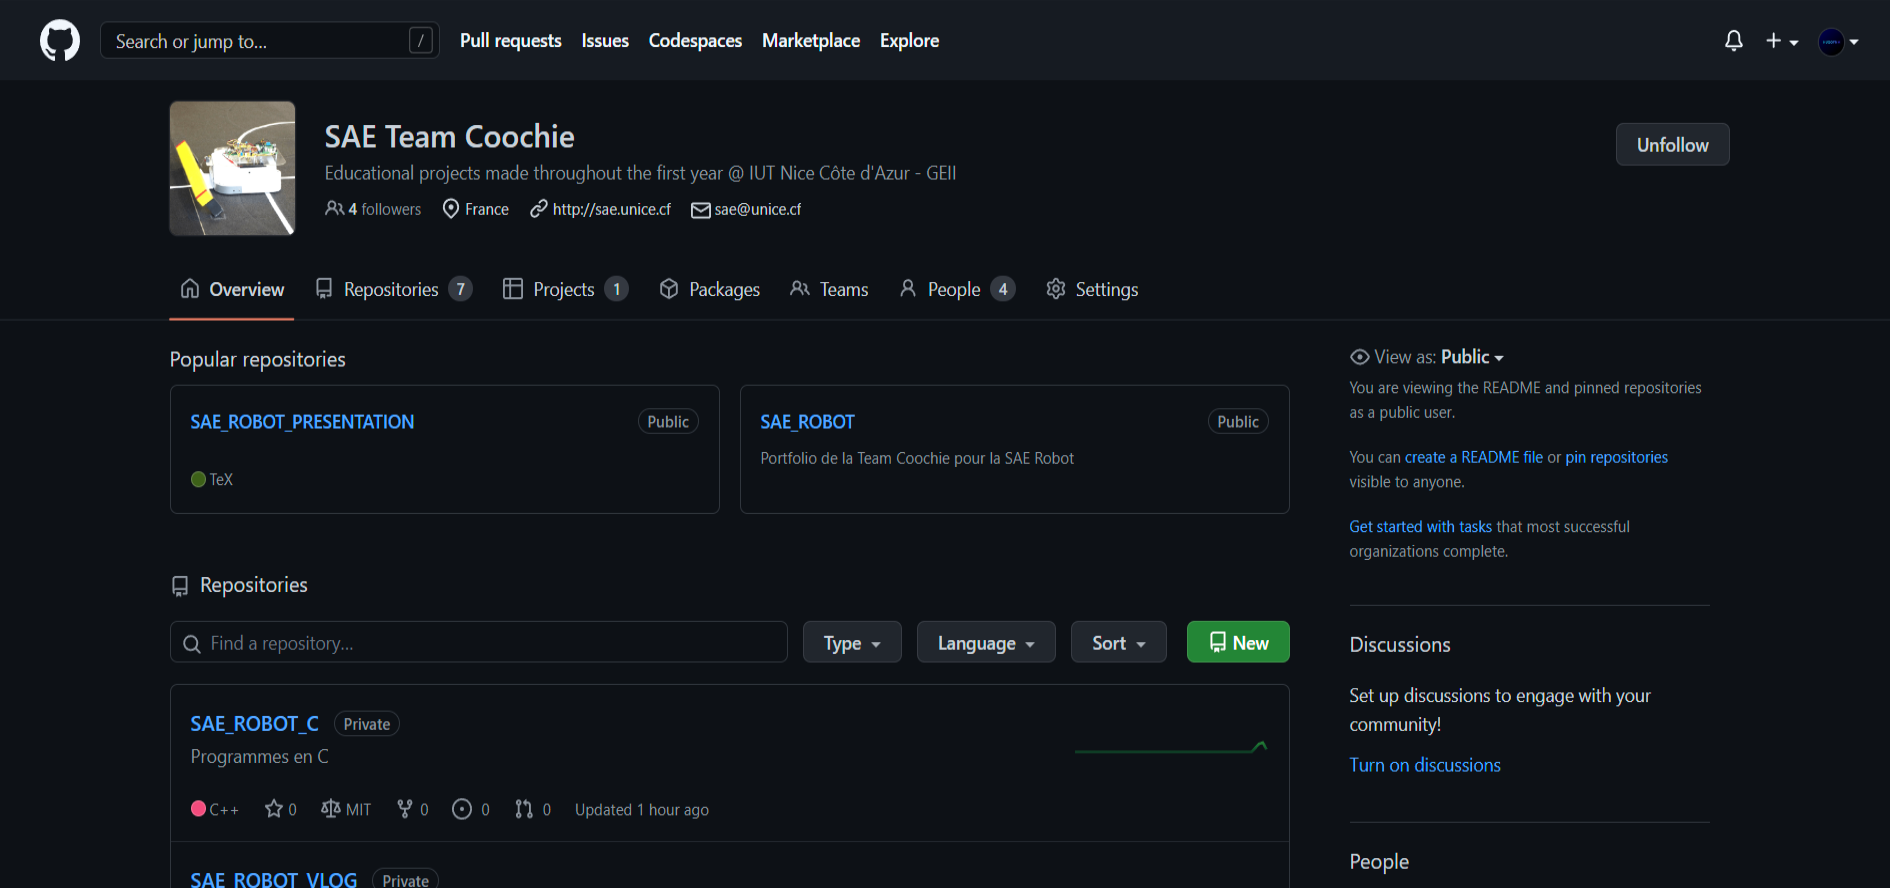
\includegraphics[width=2\linewidth]{img/sex.png}}
  \captionof{figure}{\emph{Logiciel de gestion de versions GitHub basé sur git.}}
  \label{fig:git}
\end{minipage}%
\end{figure}

\vfill
\noindent\makebox[\linewidth]{\rule{.8\paperwidth}{.6pt}}\\[0.2cm]
I.U.T. Nice Côte d'Azur - SAE Robot - 2023 \hfill goofyBot
\noindent\makebox[\linewidth]{\rule{.8\paperwidth}{.6pt}}
\newpage

\begin{figure}[H]
\centering
\begin{minipage}{.5\textwidth}
  \centering
\href{}{}  \centerline{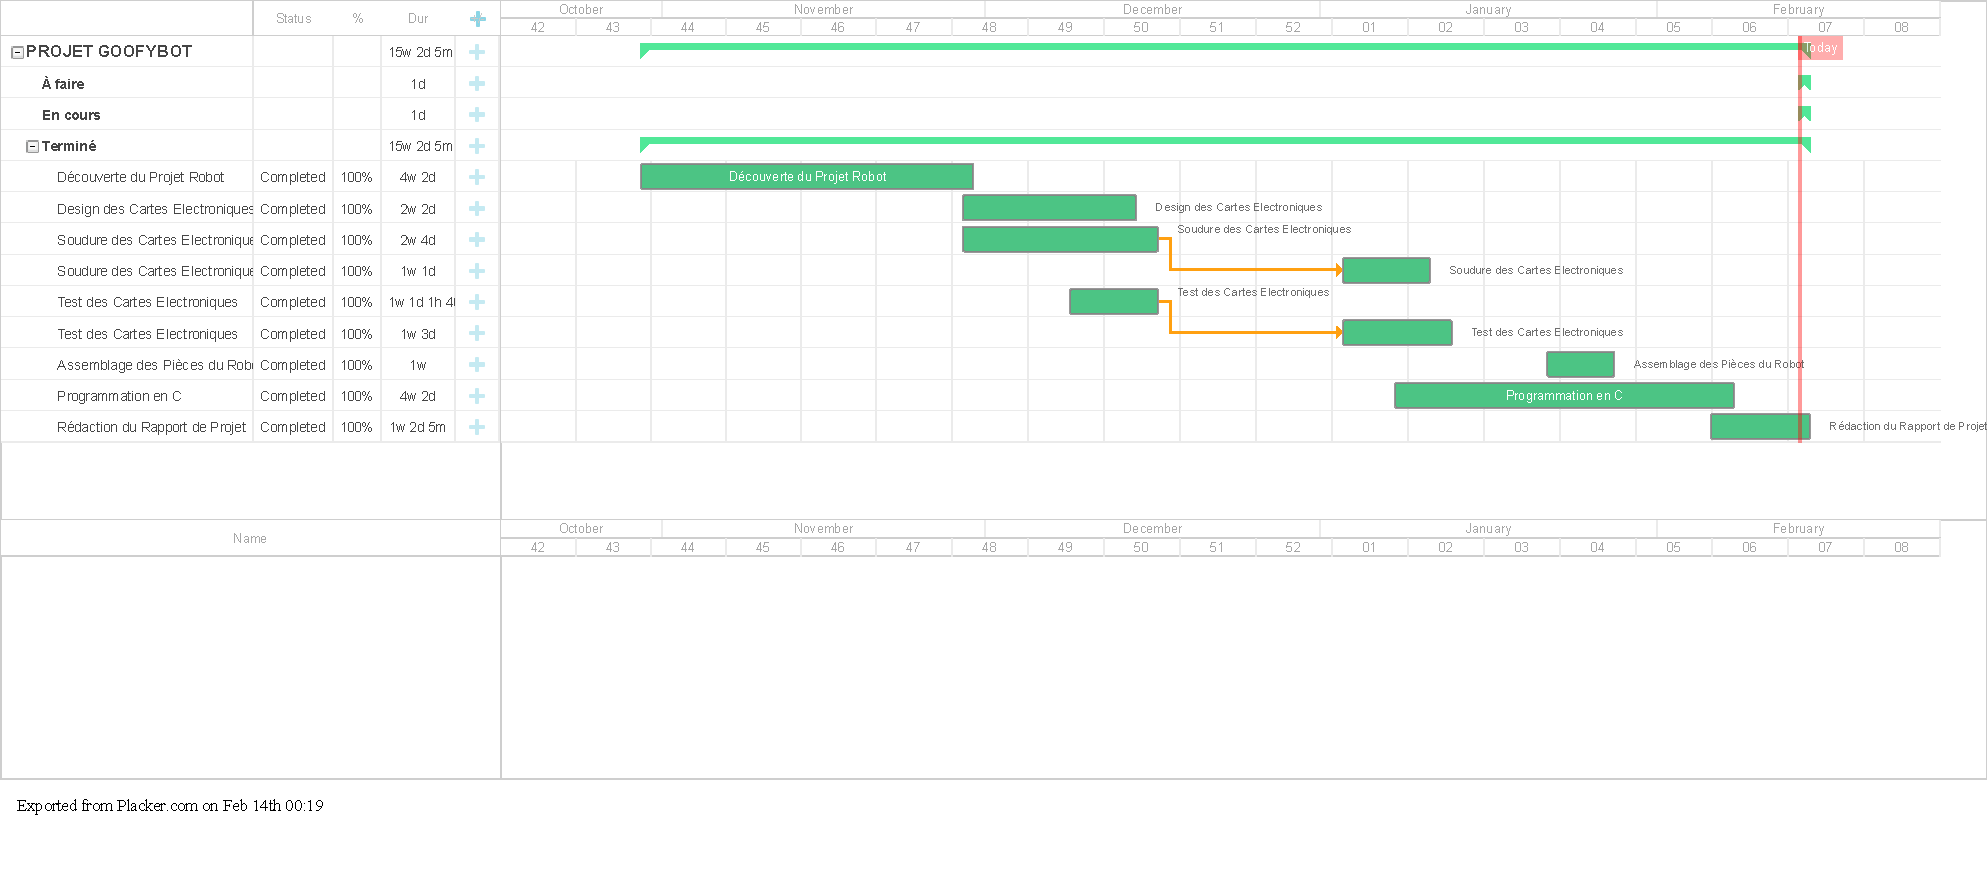
\includegraphics[width=2.5\linewidth]{pdf/gantt.pdf}}
  \captionof{figure}{\emph{GANTT.}}
  \label{fig:gantt}
\end{minipage}%
\end{figure}


\begin{figure}[H]
\centering
\begin{minipage}{.5\textwidth}
  \centering
  \centerline{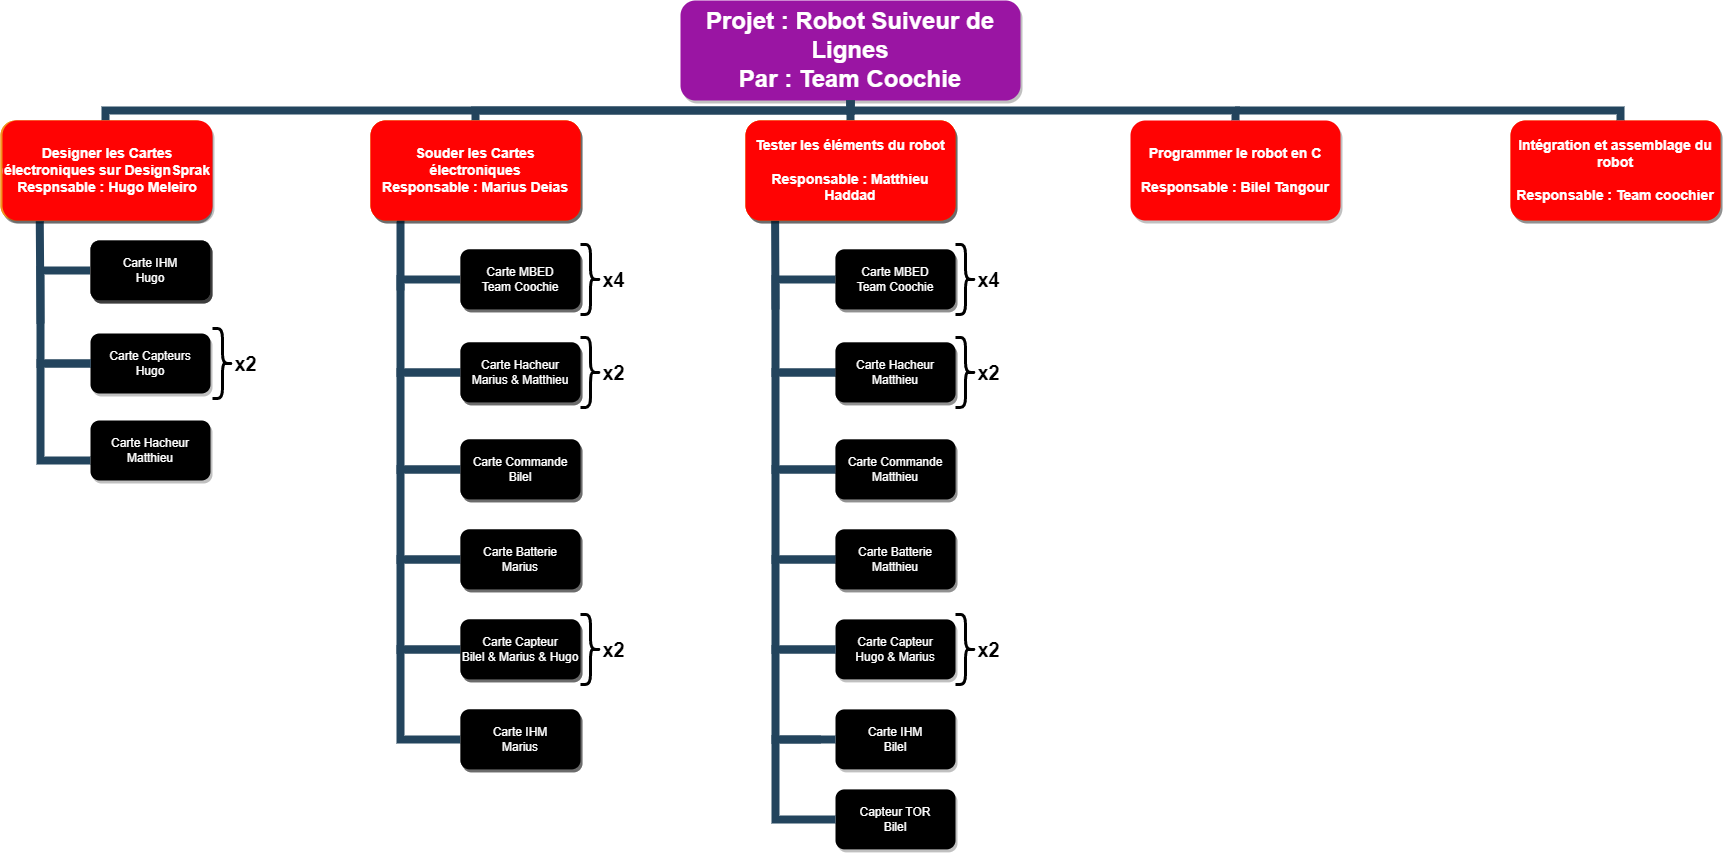
\includegraphics[width=2.5\linewidth]{img/obs.png}}
  \captionof{figure}{\emph{OBS.}}
  \label{fig:obs}
\end{minipage}%
\end{figure}

\vfill
\noindent\makebox[\linewidth]{\rule{.8\paperwidth}{.6pt}}\\[0.2cm]
I.U.T. Nice Côte d'Azur - SAE Robot - 2023 \hfill goofyBot
\noindent\makebox[\linewidth]{\rule{.8\paperwidth}{.6pt}}
\newpage
\section{Conclusion}

L'aboutissement de ce projet représente pour nous une grande première.
Certains d’entre nous ont déjà un antécédent de programmation ou d'électronique, mais cela
semble dérisoire face à tous les besoins de ce projet. Beaucoup de temps et de
travail ont été nécessaires, mais l’objectif est crucial pour la réussite de notre année. 

Même si complexe sur de nombreux points, ce projet nous a apporté beaucoup de connaissances, non seulement dans l’utilisation de logiciels comme DesignSpark PCB, TeraTerm, ARM Keil Studio, mais aussi dans le langage de programmation C++, le fonctionnement d'un microcontrôleur, ...

De plus, l'esprit de groupe est également un point important de l'apprentissage, c'est à dire savoir s'entraider, communiquer, s'organiser et planifier nos objectifs. Ce sont des points que l'on attend d'un ingénieur et qui nous seront demandés durant nos carrières professionnelles. Il est donc évident que la qualité de ce projet sera un reflet de nos capacités à évoluer au sein d'un groupe pour aller vers un même but.

Malgré les difficultés, le stress, la compétition, et parfois l'envie de casser le robot en deux, nous sommes fiers de voir notre évolution au sein de cette SAE enrichissante et vous remercions, professeurs, de nous avoir fait vivre une immersion dans le monde professionnel, le temps d'un semestre.

\noindent Merci,

\noindent L'équipe Coochie.

\vfill
\noindent\makebox[\linewidth]{\rule{.8\paperwidth}{.6pt}}\\[0.2cm]
I.U.T. Nice Côte d'Azur - SAE Robot - 2023 \hfill goofyBot
\noindent\makebox[\linewidth]{\rule{.8\paperwidth}{.6pt}}
\section{Sources \& Bibliographie}


\bibliography{}
\href{http://projet.eu.org/pedago/sin/term/6-asservissement_PID.pdf}{Explication du fonctionnement du PID}


\href{https://lms.univ-cotedazur.fr/2022/mod/resource/view.php?id=160514}{Explication de la methodologie à 
suivre}


\href{https://app.diagrams.net/}{Draw.io, utilisé pour réaliser l'OBS}


\href{https://trello.com/fr}{Trello, utilisé pour réaliser le GANTT}


\href{https://github.com/}{Github}

\vfill
\noindent\makebox[\linewidth]{\rule{.8\paperwidth}{.6pt}}\\[0.2cm]
I.U.T. Nice Côte d'Azur - SAE Robot - 2023 \hfill goofyBot
\noindent\makebox[\linewidth]{\rule{.8\paperwidth}{.6pt}}
\newpage
\section{Annexe}

\subsection{Glossaire}

\noindent \textbf{GPIO} : \emph{General Purpose Input/Output}. Les ports GPIO sont des ports d'entrées-sorties très utilisés dans le monde des microcontrôleurs, en particulier dans le domaine de l'électronique embarquée, qui ont fait leur apparition au début des années 1980. Elles sont placées sur un circuit électronique afin de communiquer avec des composants électroniques et circuits externes. Il peut s'agir de détecteurs ou senseurs pour capter des données, ou encore de contrôler des commandes.

\noindent \textbf{IHM} : \emph{Interface Homme-Machine}. C'est l'interface qui permet à l' utilisateur de communiquer avec un ordinateur, une application ou un dispositif électronique(ici un le robot suiveur de ligne). L'IHM peut prendre différentes formes, telles que des écrans graphiques, des boutons, des claviers, des écrans tactiles, des commandes vocales, etc. Le but de l'IHM est de rendre la communication avec la technologie plus intuitive et plus accessible pour les utilisateurs.



\hfill Source : Wikipédia

\subsection{Documentation}

\noindent Les liens suivants sont destinées à la documentation techniques des composants principaux de notre robot suiveur de ligne.

Sommaire :
\begin{itemize}
    \item \href{https://www.nxp.com/docs/en/data-sheet/KL25P80M48SF0.pdf}{NXP FRDM KL25Z based on Arm® Cortex®-M0+ Core}
    \item \href{https://www.st.com/resource/en/datasheet/l298.pdf}{Double Pont en H L298}
    \item \href{https://www.st.com/resource/en/datasheet/l78l.pdf}{Régulateur 5V -> 3,3V L78L}
    \item \href{https://docs.rs-online.com/8525/0900766b816ed3dd.pdf}{Régulateur 12V -> 5V TSR 1-2450}
    \item \href{https://www.mouser.fr/datasheet/2/308/1/HCPL2631_D-1522483.pdf}{Optocoupleur HCPL2631}
    \item \href{https://www.mouser.fr/datasheet/2/239/LTV_8X6_series-2887056.pdf}{Optocoupleur LTV-816}
    \item \href{https://www.ti.com/lit/gpn/lm111-n}{Comparateur de tension LM111}
\end{itemize}

\subsection{Autres}

\vfill
\noindent\makebox[\linewidth]{\rule{.8\paperwidth}{.6pt}}\\[0.2cm]
I.U.T. Nice Côte d'Azur - SAE Robot - 2023 \hfill goofyBot
\noindent\makebox[\linewidth]{\rule{.8\paperwidth}{.6pt}}

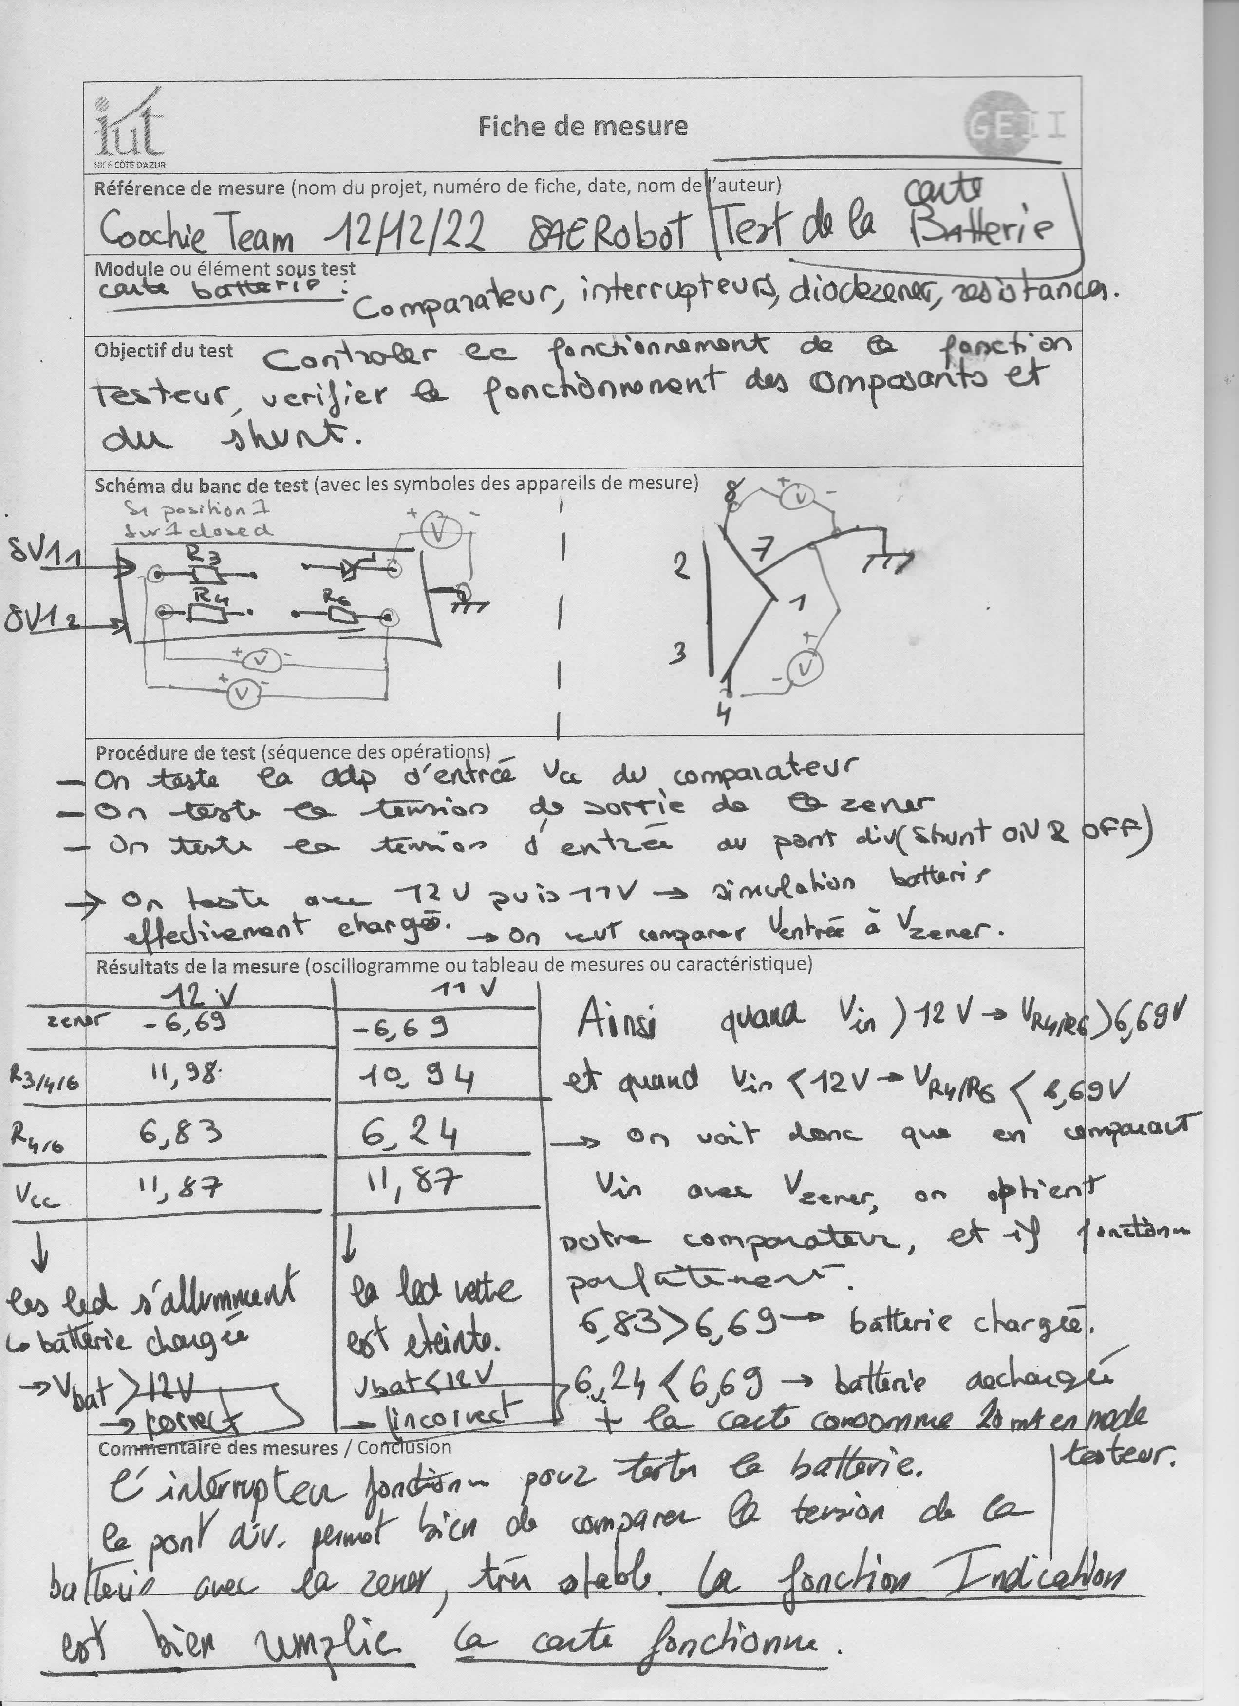
\includepdf[pages=-]{pdf/fichesmesure/degrade/Carte Batterie.pdf}

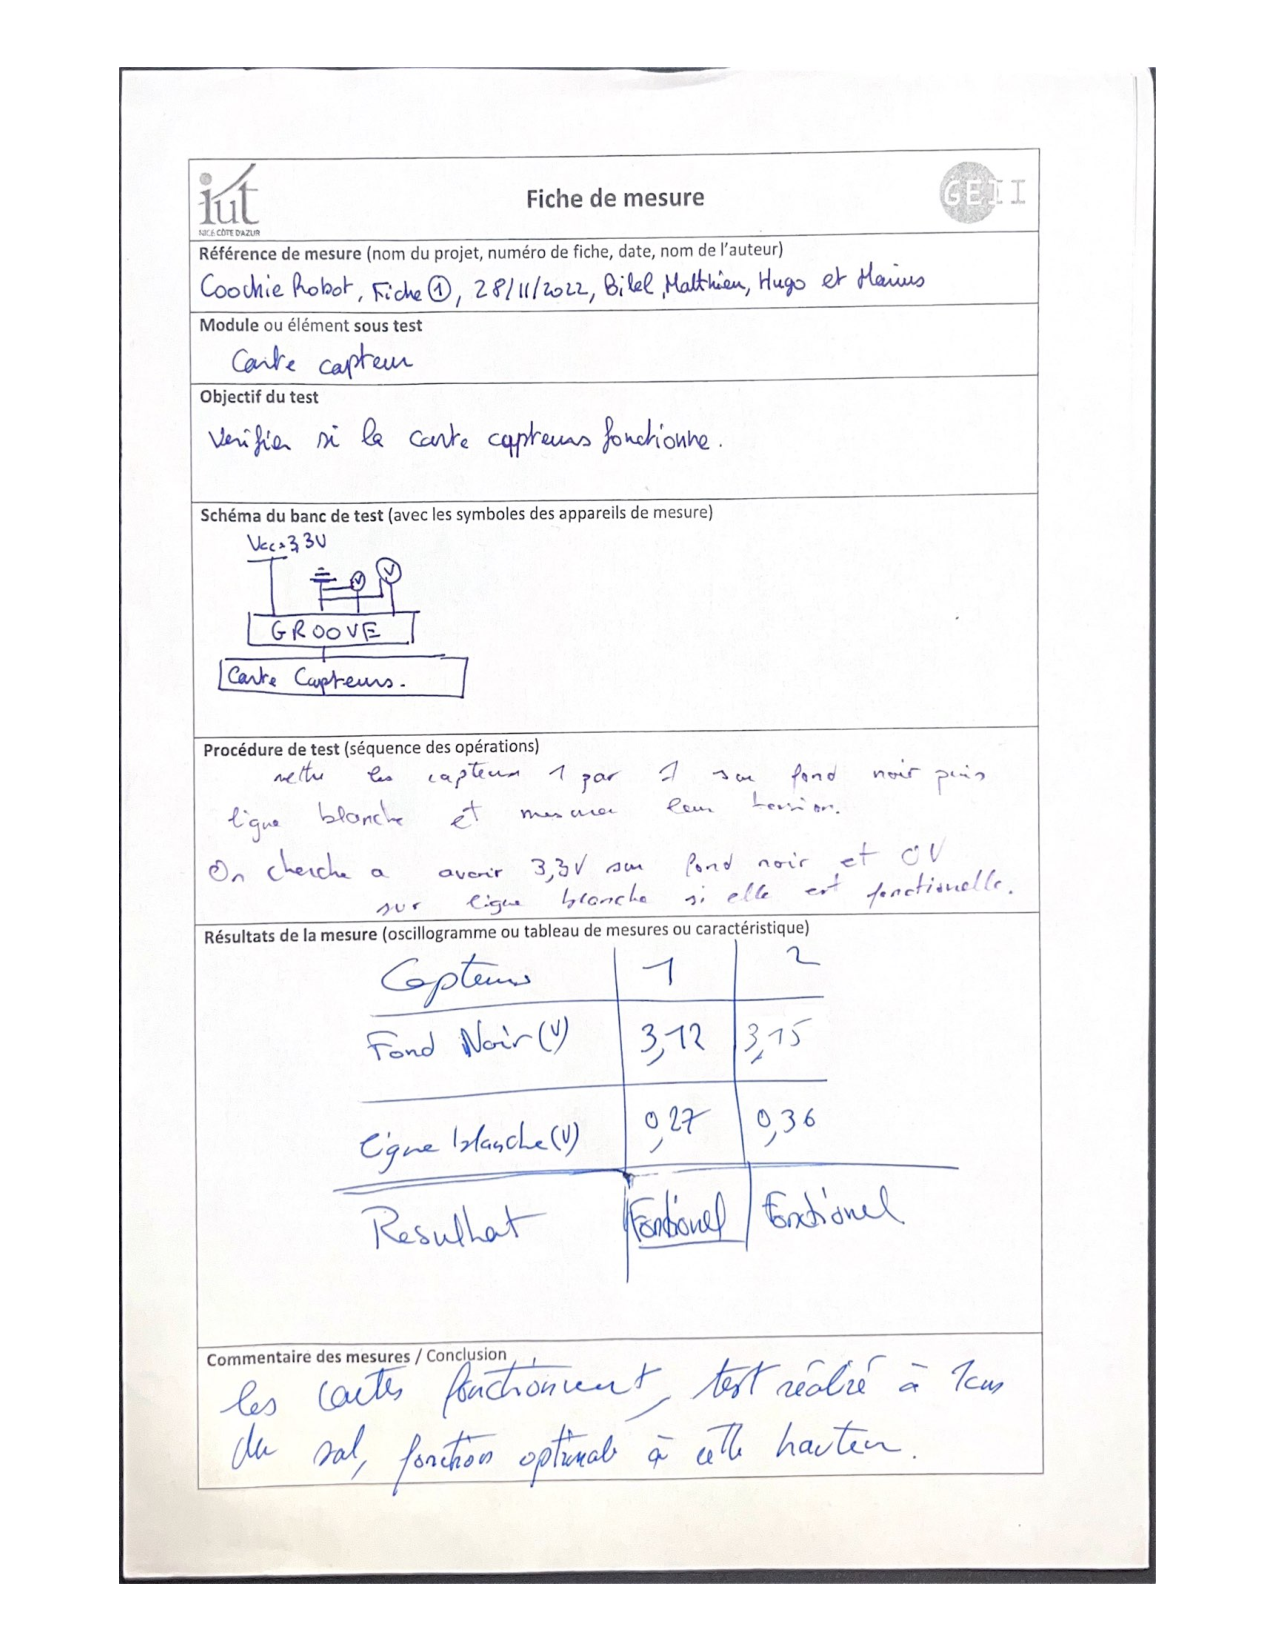
\includepdf[pages=-]{pdf/fichesmesure/degrade/Carte Capteurs.pdf}

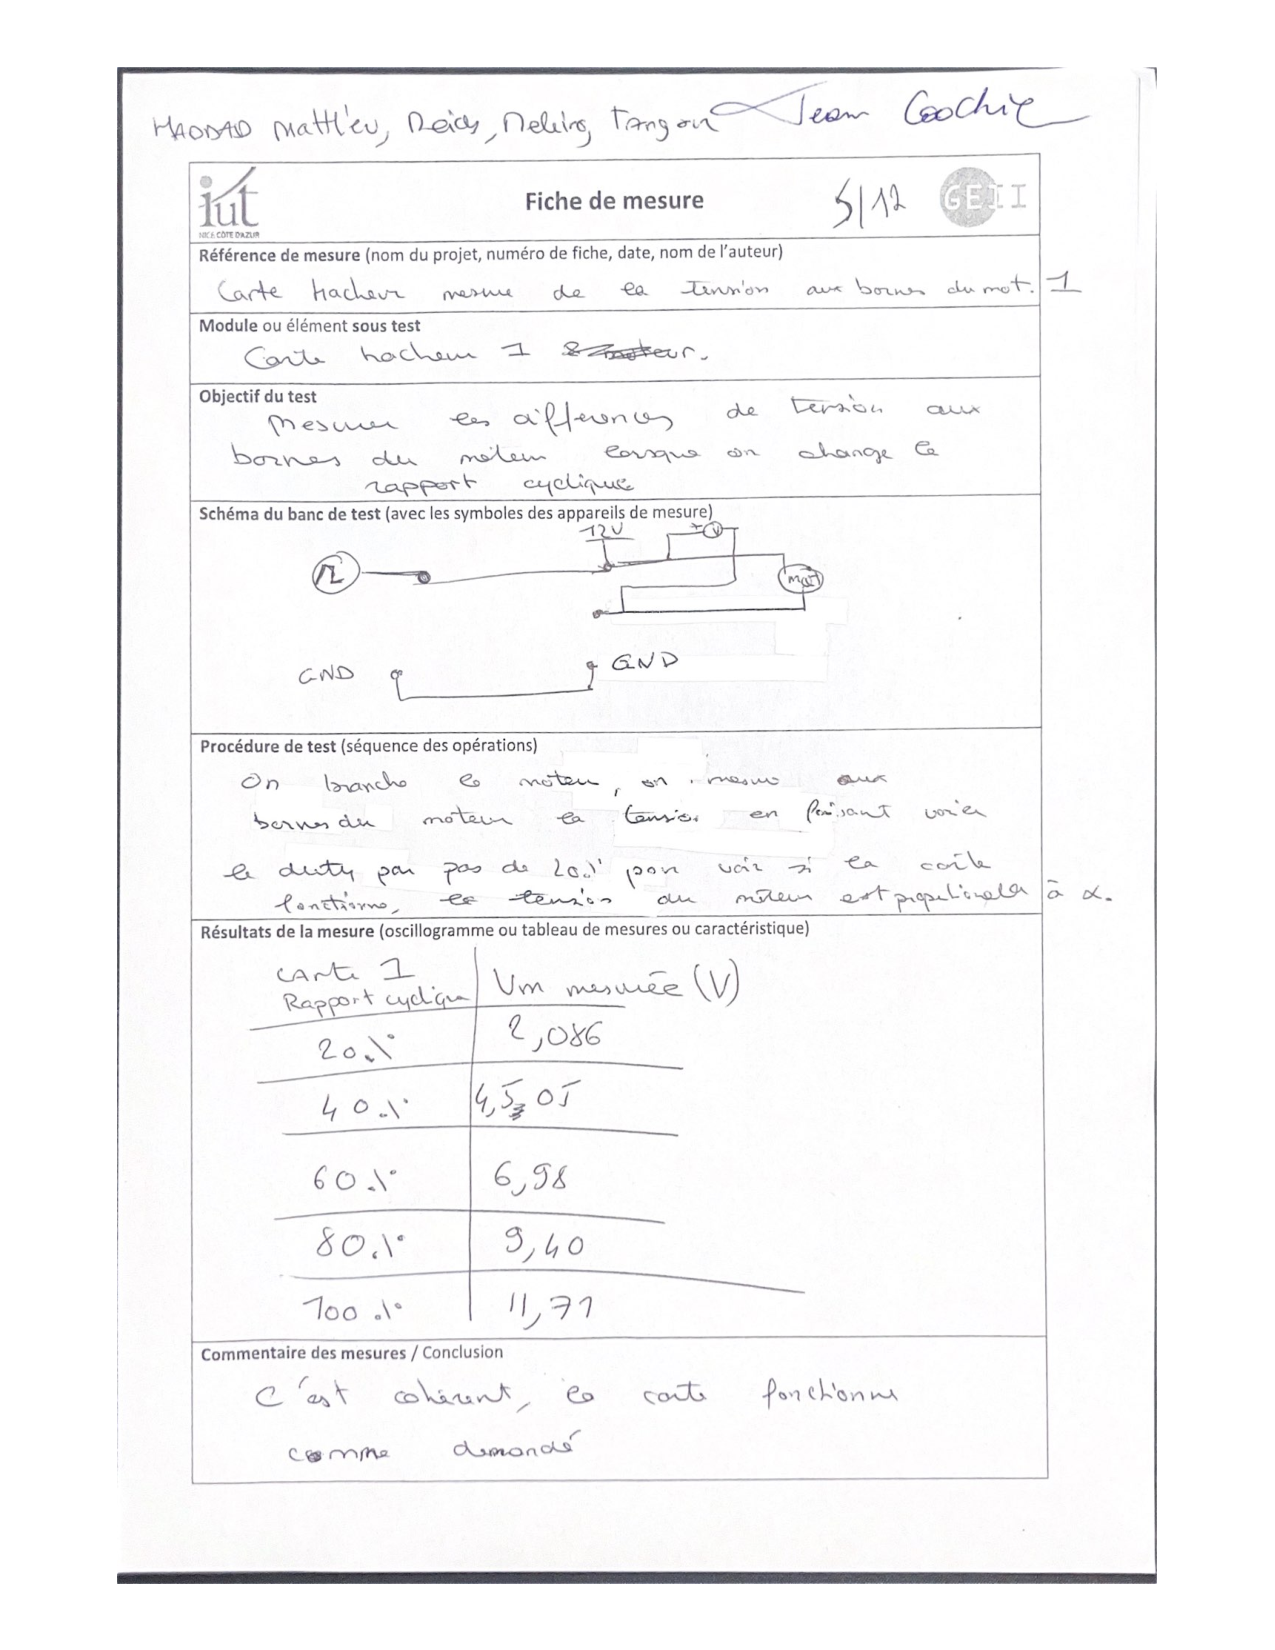
\includepdf[pages=-]{pdf/fichesmesure/degrade/Carte Hacheur.pdf}

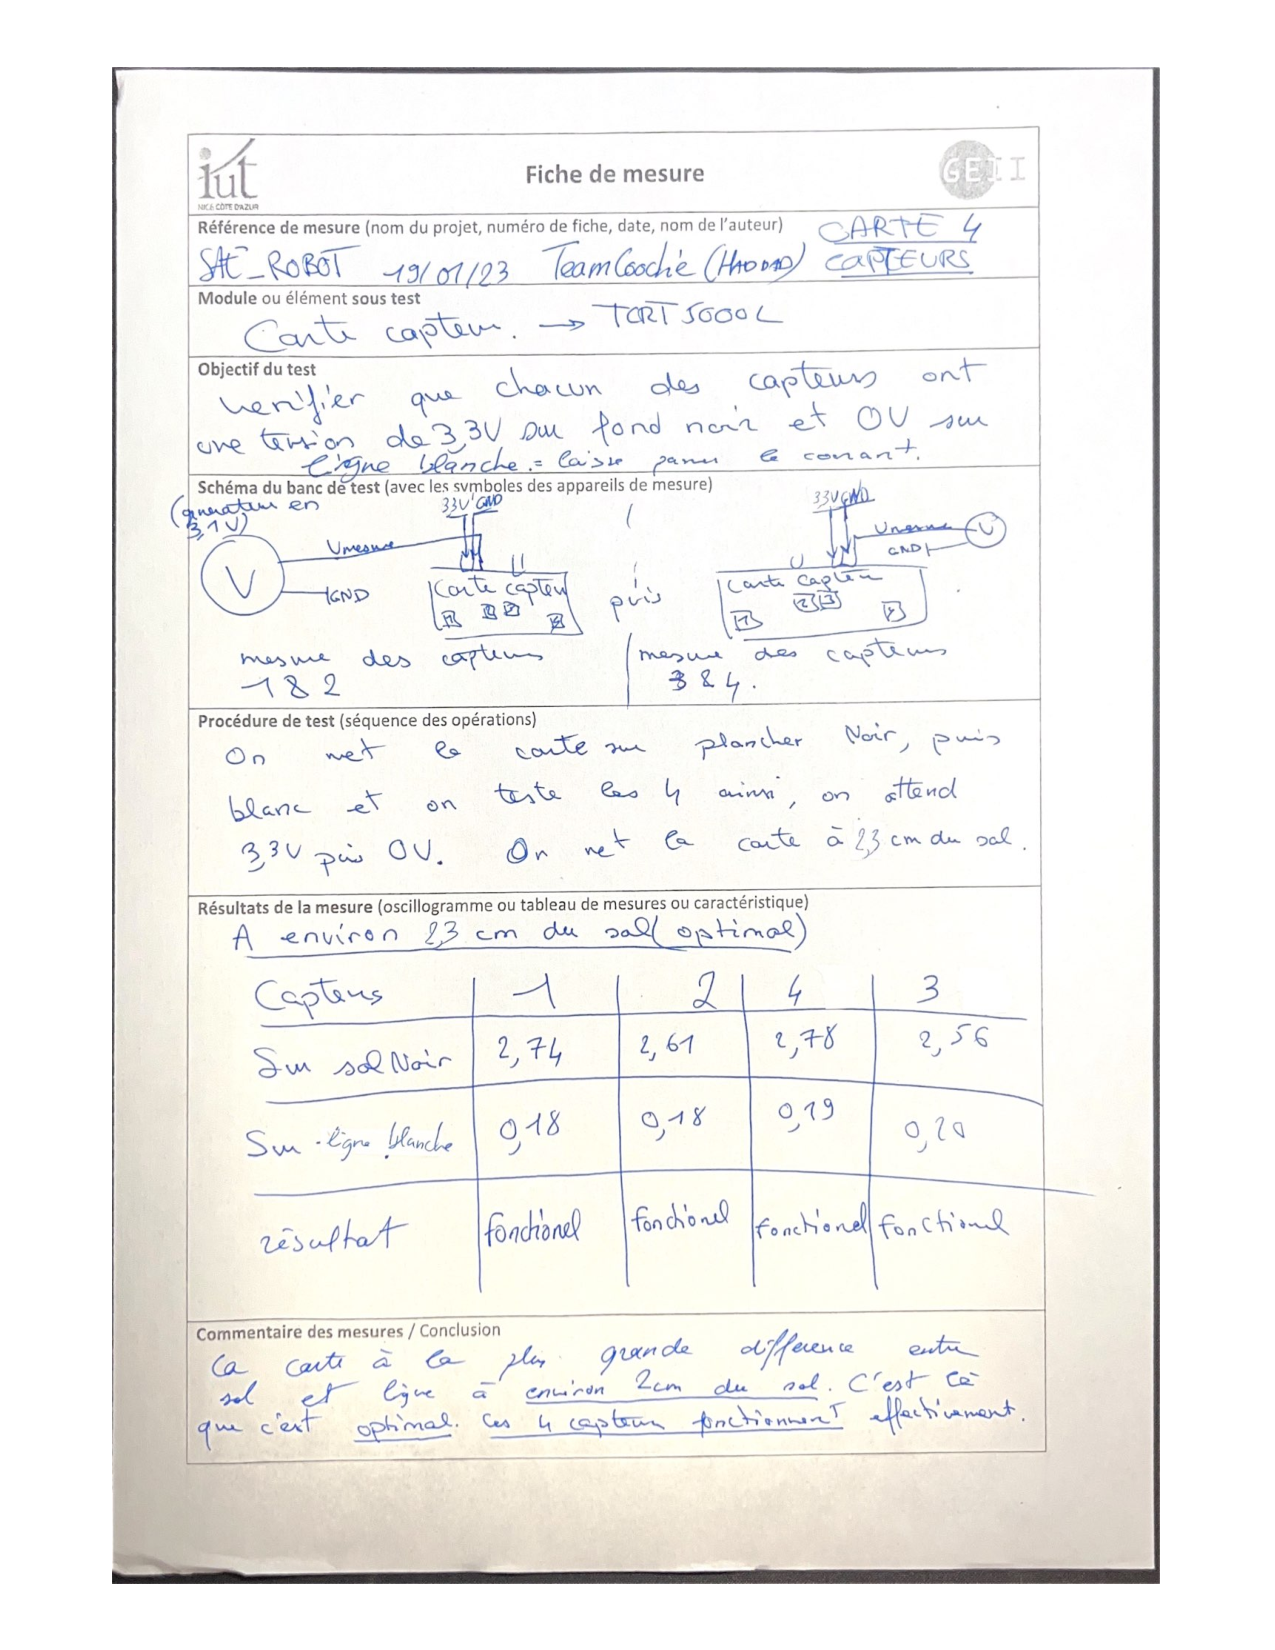
\includepdf[pages=-]{pdf/fichesmesure/designees/Carte Capteurs.pdf}

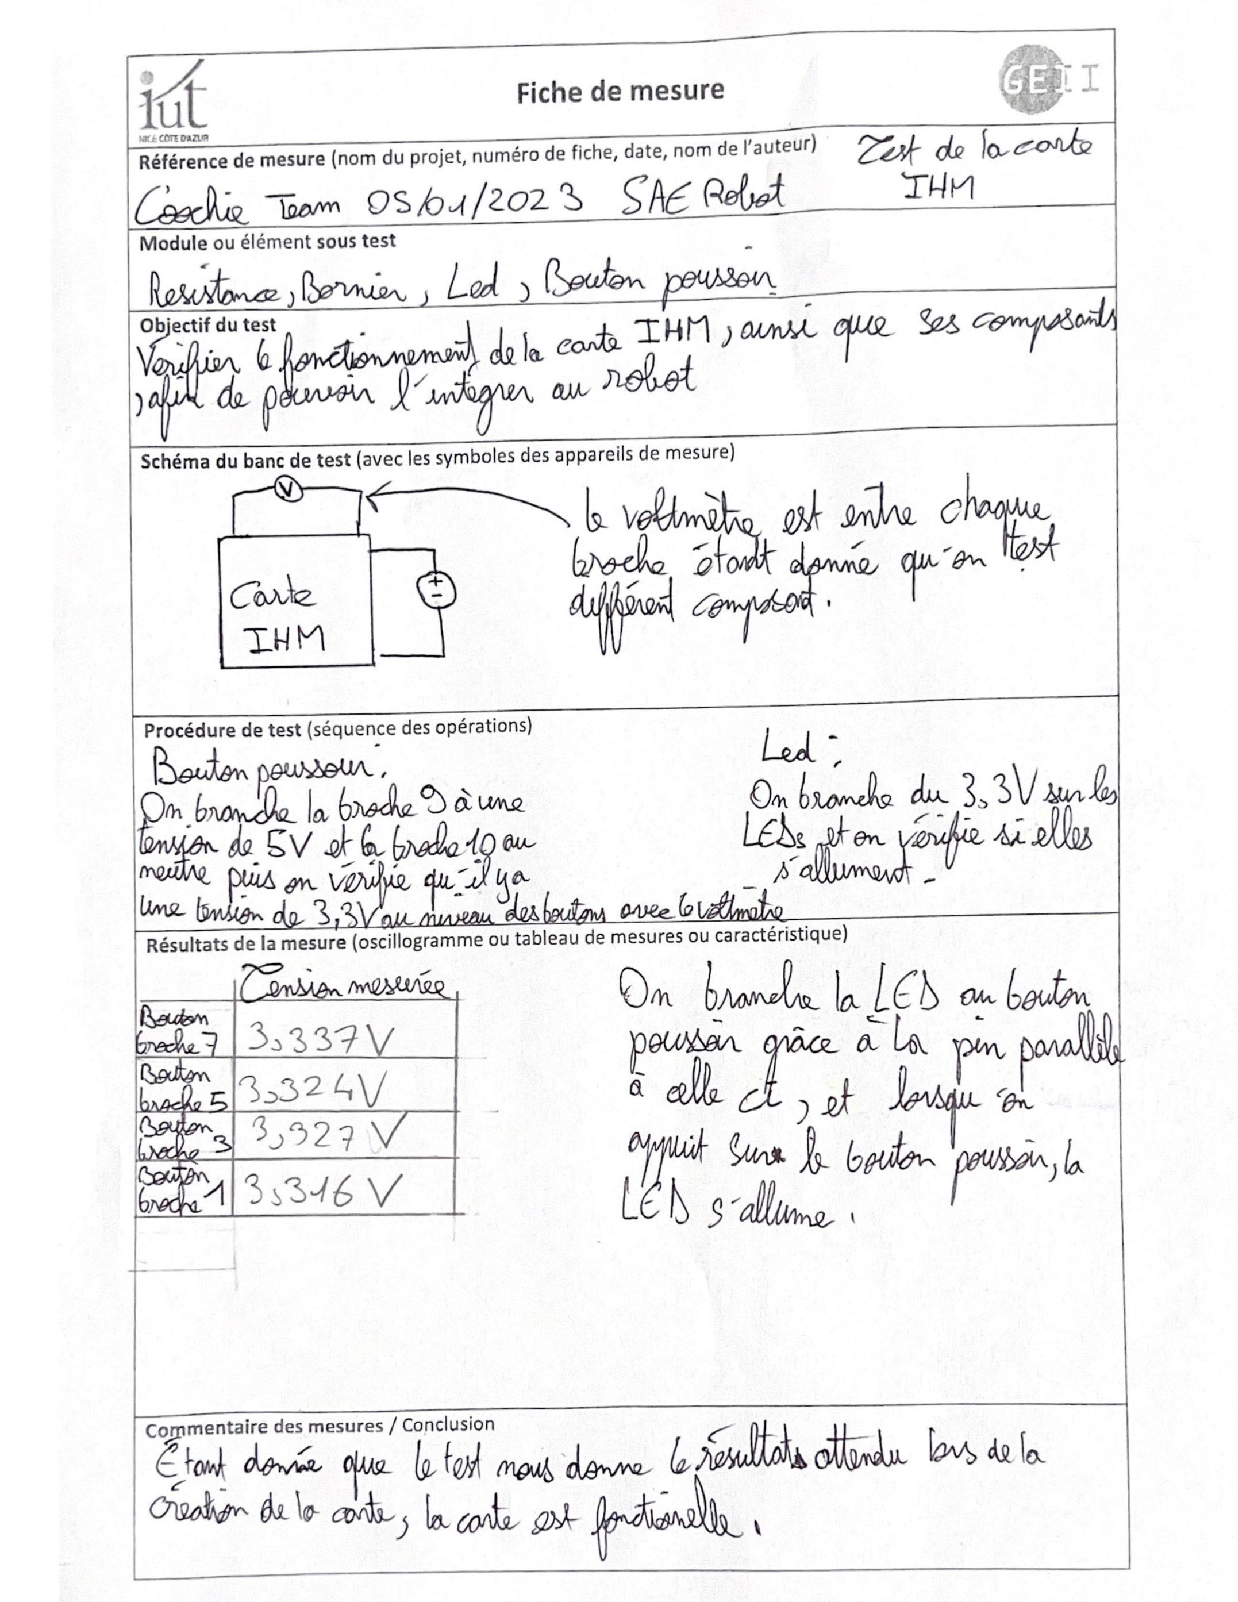
\includepdf[pages=-]{pdf/fichesmesure/designees/Carte IHM.pdf}

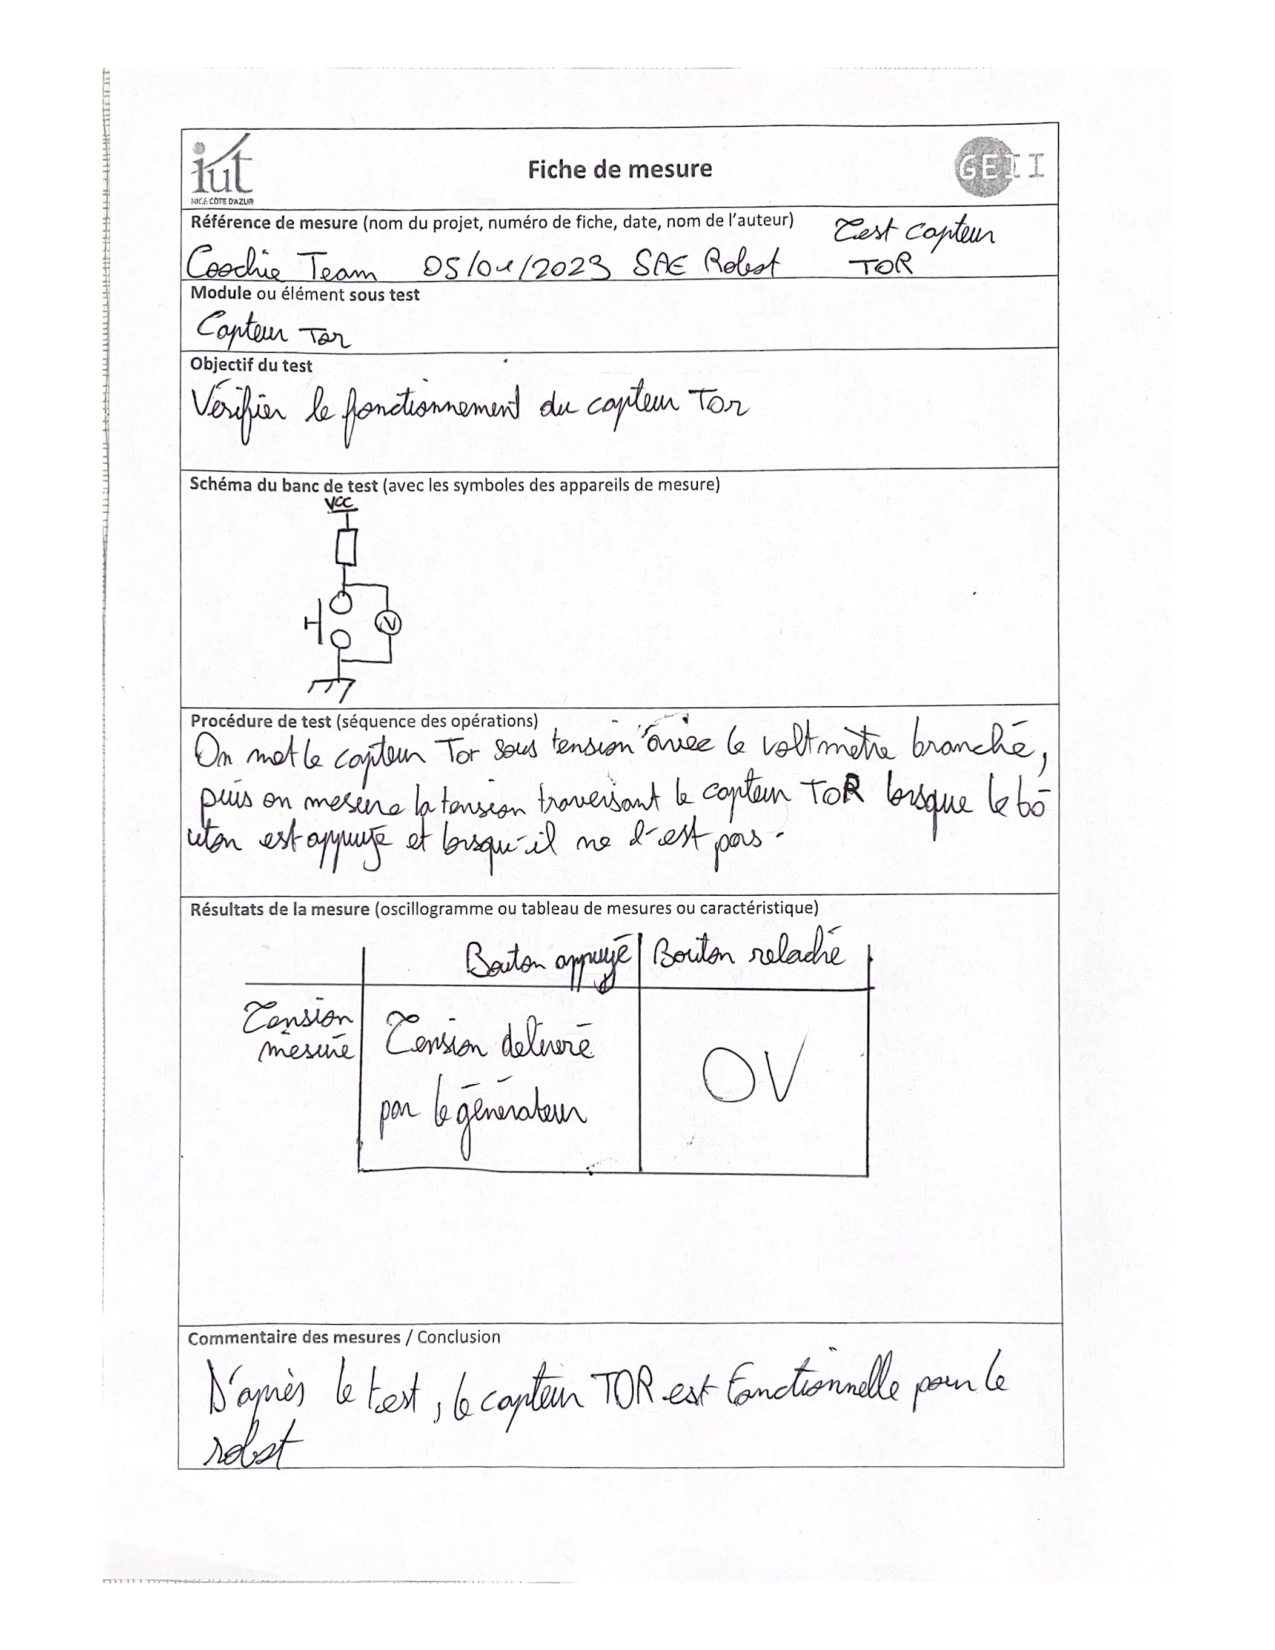
\includepdf[pages=-]{pdf/fichesmesure/designees/Capteur TOR.pdf}

\newpage

\thispagestyle{empty}
~
\vfill
\begin{center}

\large goofyBot - Coochie Team

\large I.U.T. Nice Côte d'Azur

\large 2023 | Conçu avec \LaTeX

\centering

\includegraphics[width=.3\linewidth]{img/logos/iut.png}
\end{center}


%% FIN %%
\end{document}